\documentclass[10pt,letterpaper]{article}
\usepackage[utf8]{inputenc}
\usepackage{fullpage}

\usepackage[dvipsnames]{xcolor}
\usepackage{amsmath}
\usepackage{amssymb}
\usepackage{amsfonts}
\usepackage{amsthm}
\usepackage{graphicx}
\usepackage{tikz}
\usepackage{tikz-cd}
\usetikzlibrary{calc}
\usepackage{amscd}


\newtheorem{definition}{Definition}[section]
\newtheorem{theorem}{Theorem}[section]
\newtheorem{lemma}[theorem]{Lemma}
\newtheorem{remark}[theorem]{Remark}
\newtheorem{example}[theorem]{Example}
\newtheorem{proposition}[theorem]{Proposition}

\makeatletter
\newcommand\suchthat{%
 \@ifstar
  {\mathrel{}\middle|\mathrel{}}
  {\mid}%
}
\makeatother

\newcommand{\Ceins}[1]{C_{1,#1}}
\newcommand{\Czwei}[1]{C_{2,#1}}
\newcommand{\Cdrei}[1]{C_{3,#1}}
\newcommand{\Cvier}[2]{C_{4,#1,#2}}
\newcommand{\Cfive}[2]{C_{5,#1,#2}}
% \newcommand{\Ceins}{\sqrt{n}}
% \newcommand{\Czwei}{\sqrt{2n}}



\newcommand{\Perm}{{\operatorname{Perm}}}

\newcommand{\linhull}{{\operatorname{span}}}
\newcommand{\convexhull}{{\operatorname{convex}}}

\newcommand{\Poinc}{\frakP}
\newcommand{\Bogov}{\frakB}

\newcommand{\mollifier}{\frakm}

\newcommand{\eps}{\epsilon}

\newcommand{\Id}{\rm{Id}}

\newcommand{\Lip}{\rm{Lip}}

\newcommand{\diff}{\mathop{}\!\mathrm{d}}

\DeclareMathOperator{\adj}{adj}
%\newcommand{\adj}{{\rm adj}}
\newcommand{\inv}{{-1}}
\newcommand{\invt}{{-t}}
\newcommand{\tinv}{{-t}}
\newcommand{\determinant}{{\operatorname{det}}}
\DeclareMathOperator{\Jacobian}{{\rm Jac}}
% \newcommand{\Jacobian}{{\rm Jac}}
\newcommand{\dimension}{\operatorname{dim}}
\newcommand{\sgn}{\operatorname{sgn}}
\newcommand{\adjugate}{\operatorname{adj}}
\newcommand{\sym}{\operatorname{sym}}
\newcommand{\signum}{\operatorname{sgn}}
\newcommand{\kronecker}{{\hat\delta}}
\newcommand{\dom}{\operatorname{dom}}
\newcommand{\codom}{\operatorname{codom}}
\newcommand{\rng}{\operatorname{ran}}
\newcommand{\convex}{\operatorname{convex}}
\newcommand{\coker}{\operatorname{coker}}
\newcommand{\coran}{\operatorname{coran}}

\newcommand{\dif}{{\mathrm d}}
\newcommand{\Dif}{{\mathrm D}}
\newcommand{\grad}{\operatorname{grad}}
\newcommand{\Grad}{\operatorname{Grad}}
\newcommand{\curl}{\operatorname{curl}}
\newcommand{\Curl}{\operatorname{Curl}}
\newcommand{\rot}{\curl}
\newcommand{\divergence}{\operatorname{div}}
\newcommand{\diver}{\operatorname{div}}
\newcommand{\svcurl}{\operatorname{sv-curl}}
\newcommand{\vscurl}{\operatorname{vs-curl}}
\newcommand{\sdiver}{\operatorname{sdiv}}
\newcommand{\Sdiver}{\operatorname{Sdiv}}
\newcommand{\sgrad}{\operatorname{sgrad}}
\newcommand{\Sgrad}{\operatorname{Sgrad}}
\newcommand{\Laplace}{\bigtriangleup}
\newcommand{\laplace}{\bigtriangleup}
\newcommand{\laplacian}{\laplace}
\newcommand{\Laplacian}{\laplace}
% \newcommand{\cartan}{{\mathsf d}}
% \newcommand{\cartanx}{{\mathsf d}x}
\newcommand{\cartan}{d}
\newcommand{\cartanx}{dx}

%\newcommand{\argmin}{\operatorname{argmin}}
\DeclareMathOperator*{\argmin}{{\rm argmin}}

% \DeclareMathOperator*{\carapace}{{\rm corona}}
\DeclareMathOperator*{\carapace}{{\partial \rm st}}

\newcommand{\supp}{\operatorname{supp}}
\newcommand{\esssup}{{\operatorname{esssup}}}
\newcommand{\essinf}{{\operatorname{essinf}}}

\newcommand{\equivalent}{ \Longleftrightarrow }
\newcommand{\vol}{\operatorname{vol}}
\newcommand{\st}{ \mid }
\newcommand{\diam}{{\operatorname{diam}}}
\newcommand{\height}{\operatorname{height}}
\newcommand{\dist}{\operatorname{dist}}
\newcommand{\patch}{\operatorname{st}}

\newcommand{\Trace}{\operatorname{Tr}}
\newcommand{\Tr}{\operatorname{Tr}}
\newcommand{\trace}{\operatorname{tr}}
\newcommand{\normaltrace}{\operatorname{nm}}
\newcommand{\tr}{\operatorname{tr}}
\newcommand{\Ext}{\operatorname{Ext}}
\newcommand{\Ex}{\operatorname{Ex}}
\newcommand{\ext}{\operatorname{ext}}

\newcommand{\Poincare}{\sfP}
\newcommand*{\volsphere}[1]{\color{red}{S_{#1}}}
\newcommand*{\volball}[1]{B_{#1}}

\newcommand{\subsimplex}{\calS^{\downarrow}}
\newcommand{\supsimplex}{\calS^{\uparrow}}
\newcommand{\supersimplex}{\supsimplex}
\newcommand{\orientation}{\mathscr{O}}
\newcommand{\restrict}{R}

\newcommand{\Mesh}{\calT}
\newcommand{\Vertices}{\calV}
\newcommand{\Edges}{\calE}
\newcommand{\Faces}{\calF}
\newcommand{\Ball}{\calB}
\newcommand{\Sphere}{S}
\newcommand{\underlying}[1]{\left| #1 \right|}

\newcommand{\Distr}{\calD}
\newcommand{\Cont}{\calC}
\newcommand{\Lebesgue}{L}
\newcommand{\Sobolev}{W}
\newcommand{\SOBOLEV}{\bfW}
\newcommand{\SobolevLambda}{W\Lambda}
\newcommand{\Alt}{\Lambda}
\newcommand{\loc}{\rm{loc}}

\newcommand{\Ned}{{\calN d}}
\newcommand{\RT}{{\calR T}}
\newcommand{\BDM}{{\calB \calD \calM}}
  

\newcommand*{\ConstantPF}{C_{\rm{PF}}}







\newcommand{\bbA}{{\mathbb A}}
\newcommand{\bbB}{{\mathbb B}}
\newcommand{\bbC}{{\mathbb C}}
\newcommand{\bbD}{{\mathbb D}}
\newcommand{\bbE}{{\mathbb E}}
\newcommand{\bbF}{{\mathbb F}}
\newcommand{\bbG}{{\mathbb G}}
\newcommand{\bbH}{{\mathbb H}}
\newcommand{\bbI}{{\mathbb I}}
\newcommand{\bbJ}{{\mathbb J}}
\newcommand{\bbK}{{\mathbb K}}
\newcommand{\bbL}{{\mathbb L}}
\newcommand{\bbM}{{\mathbb M}}
\newcommand{\bbN}{{\mathbb N}}
\newcommand{\bbO}{{\mathbb O}}
\newcommand{\bbP}{{\mathbb P}}
\newcommand{\bbQ}{{\mathbb Q}}
\newcommand{\bbR}{{\mathbb R}}
\newcommand{\bbS}{{\mathbb S}}
\newcommand{\bbT}{{\mathbb T}}
\newcommand{\bbU}{{\mathbb U}}
\newcommand{\bbV}{{\mathbb V}}
\newcommand{\bbW}{{\mathbb W}}
\newcommand{\bbX}{{\mathbb X}}
\newcommand{\bbY}{{\mathbb Y}}
\newcommand{\bbZ}{{\mathbb Z}}

\newcommand{\bfA}{{\mathbf A}}
\newcommand{\bfB}{{\mathbf B}}
\newcommand{\bfC}{{\mathbf C}}
\newcommand{\bfD}{{\mathbf D}}
\newcommand{\bfE}{{\mathbf E}}
\newcommand{\bfF}{{\mathbf F}}
\newcommand{\bfG}{{\mathbf G}}
\newcommand{\bfH}{{\mathbf H}}
\newcommand{\bfI}{{\mathbf I}}
\newcommand{\bfJ}{{\mathbf J}}
\newcommand{\bfK}{{\mathbf K}}
\newcommand{\bfL}{{\mathbf L}}
\newcommand{\bfM}{{\mathbf M}}
\newcommand{\bfN}{{\mathbf N}}
\newcommand{\bfO}{{\mathbf O}}
\newcommand{\bfP}{{\mathbf P}}
\newcommand{\bfQ}{{\mathbf Q}}
\newcommand{\bfR}{{\mathbf R}}
\newcommand{\bfS}{{\mathbf S}}
\newcommand{\bfT}{{\mathbf T}}
\newcommand{\bfU}{{\mathbf U}}
\newcommand{\bfV}{{\mathbf V}}
\newcommand{\bfW}{{\mathbf W}}
\newcommand{\bfX}{{\mathbf X}}
\newcommand{\bfY}{{\mathbf Y}}
\newcommand{\bfZ}{{\mathbf Z}}

\newcommand{\bfa}{{\mathbf a}}
\newcommand{\bfb}{{\mathbf b}}
\newcommand{\bfc}{{\mathbf c}}
\newcommand{\bfd}{{\mathbf d}}
\newcommand{\bfe}{{\mathbf e}}
\newcommand{\bff}{{\mathbf f}}
\newcommand{\bfg}{{\mathbf g}}
\newcommand{\bfh}{{\mathbf h}}
\newcommand{\bfi}{{\mathbf i}}
\newcommand{\bfj}{{\mathbf j}}
\newcommand{\bfk}{{\mathbf k}}
\newcommand{\bfl}{{\mathbf l}}
\newcommand{\bfm}{{\mathbf m}}
\newcommand{\bfn}{{\mathbf n}}
\newcommand{\bfo}{{\mathbf o}}
\newcommand{\bfp}{{\mathbf p}}
\newcommand{\bfq}{{\mathbf q}}
\newcommand{\bfr}{{\mathbf r}}
\newcommand{\bfs}{{\mathbf s}}
\newcommand{\bft}{{\mathbf t}}
\newcommand{\bfu}{{\mathbf u}}
\newcommand{\bfv}{{\mathbf v}}
\newcommand{\bfw}{{\mathbf w}}
\newcommand{\bfx}{{\mathbf x}}
\newcommand{\bfy}{{\mathbf y}}
\newcommand{\bfz}{{\mathbf z}}


\newcommand{\calA}{{\mathcal A}}
\newcommand{\calB}{{\mathcal B}}
\newcommand{\calC}{{\mathcal C}}
\newcommand{\calD}{{\mathcal D}}
\newcommand{\calE}{{\mathcal E}}
\newcommand{\calF}{{\mathcal F}}
\newcommand{\calG}{{\mathcal G}}
\newcommand{\calH}{{\mathcal H}}
\newcommand{\calI}{{\mathcal I}}
\newcommand{\calJ}{{\mathcal J}}
\newcommand{\calK}{{\mathcal K}}
\newcommand{\calL}{{\mathcal L}}
\newcommand{\calM}{{\mathcal M}}
\newcommand{\calN}{{\mathcal N}}
\newcommand{\calO}{{\mathcal O}}
\newcommand{\calP}{{\mathcal P}}
\newcommand{\calQ}{{\mathcal Q}}
\newcommand{\calR}{{\mathcal R}}
\newcommand{\calS}{{\mathcal S}}
\newcommand{\calT}{{\mathcal T}}
\newcommand{\calU}{{\mathcal U}}
\newcommand{\calV}{{\mathcal V}}
\newcommand{\calW}{{\mathcal W}}
\newcommand{\calX}{{\mathcal X}}
\newcommand{\calY}{{\mathcal Y}}
\newcommand{\calZ}{{\mathcal Z}}

\newcommand{\fraka}{{\mathfrak a}}
\newcommand{\frakb}{{\mathfrak b}}
\newcommand{\frakc}{{\mathfrak c}}
\newcommand{\frakd}{{\mathfrak d}}
\newcommand{\frake}{{\mathfrak e}}
\newcommand{\frakf}{{\mathfrak f}}
\newcommand{\frakg}{{\mathfrak g}}
\newcommand{\frakh}{{\mathfrak h}}
\newcommand{\fraki}{{\mathfrak i}}
\newcommand{\frakj}{{\mathfrak j}}
\newcommand{\frakk}{{\mathfrak k}}
\newcommand{\frakl}{{\mathfrak l}}
\newcommand{\frakm}{{\mathfrak m}}
\newcommand{\frakn}{{\mathfrak n}}
\newcommand{\frako}{{\mathfrak o}}
\newcommand{\frakp}{{\mathfrak p}}
\newcommand{\frakq}{{\mathfrak q}}
\newcommand{\frakr}{{\mathfrak r}}
\newcommand{\fraks}{{\mathfrak s}}
\newcommand{\frakt}{{\mathfrak t}}
\newcommand{\fraku}{{\mathfrak u}}
\newcommand{\frakv}{{\mathfrak v}}
\newcommand{\frakw}{{\mathfrak w}}
\newcommand{\frakx}{{\mathfrak x}}
\newcommand{\fraky}{{\mathfrak y}}
\newcommand{\frakz}{{\mathfrak z}}
\newcommand{\frakA}{{\mathfrak A}}
\newcommand{\frakB}{{\mathfrak B}}
\newcommand{\frakC}{{\mathfrak C}}
\newcommand{\frakD}{{\mathfrak D}}
\newcommand{\frakE}{{\mathfrak E}}
\newcommand{\frakF}{{\mathfrak F}}
\newcommand{\frakG}{{\mathfrak G}}
\newcommand{\frakH}{{\mathfrak H}}
\newcommand{\frakI}{{\mathfrak I}}
\newcommand{\frakJ}{{\mathfrak J}}
\newcommand{\frakK}{{\mathfrak K}}
\newcommand{\frakL}{{\mathfrak L}}
\newcommand{\frakM}{{\mathfrak M}}
\newcommand{\frakN}{{\mathfrak N}}
\newcommand{\frakO}{{\mathfrak O}}
\newcommand{\frakP}{{\mathfrak P}}
\newcommand{\frakQ}{{\mathfrak Q}}
\newcommand{\frakR}{{\mathfrak R}}
\newcommand{\frakS}{{\mathfrak S}}
\newcommand{\frakT}{{\mathfrak T}}
\newcommand{\frakU}{{\mathfrak U}}
\newcommand{\frakV}{{\mathfrak V}}
\newcommand{\frakW}{{\mathfrak W}}
\newcommand{\frakX}{{\mathfrak X}}
\newcommand{\frakY}{{\mathfrak Y}}
\newcommand{\frakZ}{{\mathfrak Z}}







\newcommand{\rma}{{\mathrm a}}
\newcommand{\rmb}{{\mathrm b}}
\newcommand{\rmc}{{\mathrm c}}
\newcommand{\rmd}{{\mathrm d}}
\newcommand{\rme}{{\mathrm e}}
\newcommand{\rmf}{{\mathrm f}}
\newcommand{\rmg}{{\mathrm g}}
\newcommand{\rmh}{{\mathrm h}}
\newcommand{\rmi}{{\mathrm i}}
\newcommand{\rmj}{{\mathrm j}}
\newcommand{\rmk}{{\mathrm k}}
\newcommand{\rml}{{\mathrm l}}
\newcommand{\rmm}{{\mathrm m}}
\newcommand{\rmn}{{\mathrm n}}
\newcommand{\rmo}{{\mathrm o}}
\newcommand{\rmp}{{\mathrm p}}
\newcommand{\rmq}{{\mathrm q}}
\newcommand{\rmr}{{\mathrm r}}
\newcommand{\rms}{{\mathrm s}}
\newcommand{\rmt}{{\mathrm t}}
\newcommand{\rmu}{{\mathrm u}}
\newcommand{\rmv}{{\mathrm v}}
\newcommand{\rmw}{{\mathrm w}}
\newcommand{\rmx}{{\mathrm x}}
\newcommand{\rmy}{{\mathrm y}}
\newcommand{\rmz}{{\mathrm z}}
\newcommand{\rmA}{{\mathrm A}}
\newcommand{\rmB}{{\mathrm B}}
\newcommand{\rmC}{{\mathrm C}}
\newcommand{\rmD}{{\mathrm D}}
\newcommand{\rmE}{{\mathrm E}}
\newcommand{\rmF}{{\mathrm F}}
\newcommand{\rmG}{{\mathrm G}}
\newcommand{\rmH}{{\mathrm H}}
\newcommand{\rmI}{{\mathrm I}}
\newcommand{\rmJ}{{\mathrm J}}
\newcommand{\rmK}{{\mathrm K}}
\newcommand{\rmL}{{\mathrm L}}
\newcommand{\rmM}{{\mathrm M}}
\newcommand{\rmN}{{\mathrm N}}
\newcommand{\rmO}{{\mathrm O}}
\newcommand{\rmP}{{\mathrm P}}
\newcommand{\rmQ}{{\mathrm Q}}
\newcommand{\rmR}{{\mathrm R}}
\newcommand{\rmS}{{\mathrm S}}
\newcommand{\rmT}{{\mathrm T}}
\newcommand{\rmU}{{\mathrm U}}
\newcommand{\rmV}{{\mathrm V}}
\newcommand{\rmW}{{\mathrm W}}
\newcommand{\rmX}{{\mathrm X}}
\newcommand{\rmY}{{\mathrm Y}}
\newcommand{\rmZ}{{\mathrm Z}}





\newcommand{\scrA}{{\mathscr A}}
\newcommand{\scrB}{{\mathscr B}}
\newcommand{\scrC}{{\mathscr C}}
\newcommand{\scrD}{{\mathscr D}}
\newcommand{\scrE}{{\mathscr E}}
\newcommand{\scrF}{{\mathscr F}}
\newcommand{\scrG}{{\mathscr G}}
\newcommand{\scrH}{{\mathscr H}}
\newcommand{\scrI}{{\mathscr I}}
\newcommand{\scrJ}{{\mathscr J}}
\newcommand{\scrK}{{\mathscr K}}
\newcommand{\scrL}{{\mathscr L}}
\newcommand{\scrM}{{\mathscr M}}
\newcommand{\scrN}{{\mathscr N}}
\newcommand{\scrO}{{\mathscr O}}
\newcommand{\scrP}{{\mathscr P}}
\newcommand{\scrQ}{{\mathscr Q}}
\newcommand{\scrR}{{\mathscr R}}
\newcommand{\scrS}{{\mathscr S}}
\newcommand{\scrT}{{\mathscr T}}
\newcommand{\scrU}{{\mathscr U}}
\newcommand{\scrV}{{\mathscr V}}
\newcommand{\scrW}{{\mathscr W}}
\newcommand{\scrX}{{\mathscr X}}
\newcommand{\scrY}{{\mathscr Y}}
\newcommand{\scrZ}{{\mathscr Z}}


\newcommand{\veca}{{\vec a}}
\newcommand{\vecb}{{\vec b}}
\newcommand{\vecc}{{\vec c}}
\newcommand{\vecd}{{\vec d}}
\newcommand{\vece}{{\vec e}}
\newcommand{\vecf}{{\vec f}}
\newcommand{\vecg}{{\vec g}}
\newcommand{\vech}{{\vec h}}
\newcommand{\veci}{{\vec i}}
\newcommand{\vecj}{{\vec j}}
\newcommand{\veck}{{\vec k}}
\newcommand{\vecl}{{\vec l}}
\newcommand{\vecm}{{\vec m}}
\newcommand{\vecn}{{\vec n}}
\newcommand{\veco}{{\vec o}}
\newcommand{\vecp}{{\vec p}}
\newcommand{\vecq}{{\vec q}}
\newcommand{\vecr}{{\vec r}}
\newcommand{\vecs}{{\vec s}}
\newcommand{\vect}{{\vec t}}
\newcommand{\vecu}{{\vec u}}
\newcommand{\vecv}{{\vec v}}
\newcommand{\vecw}{{\vec w}}
\newcommand{\vecx}{{\vec x}}
\newcommand{\vecy}{{\vec y}}
\newcommand{\vecz}{{\vec z}}
\newcommand{\vecA}{{\vec A}}
\newcommand{\vecB}{{\vec B}}
\newcommand{\vecC}{{\vec C}}
\newcommand{\vecD}{{\vec D}}
\newcommand{\vecE}{{\vec E}}
\newcommand{\vecF}{{\vec F}}
\newcommand{\vecG}{{\vec G}}
\newcommand{\vecH}{{\vec H}}
\newcommand{\vecI}{{\vec I}}
\newcommand{\vecJ}{{\vec J}}
\newcommand{\vecK}{{\vec K}}
\newcommand{\vecL}{{\vec L}}
\newcommand{\vecM}{{\vec M}}
\newcommand{\vecN}{{\vec N}}
\newcommand{\vecO}{{\vec O}}
\newcommand{\vecP}{{\vec P}}
\newcommand{\vecQ}{{\vec Q}}
\newcommand{\vecR}{{\vec R}}
\newcommand{\vecS}{{\vec S}}
\newcommand{\vecT}{{\vec T}}
\newcommand{\vecU}{{\vec U}}
\newcommand{\vecV}{{\vec V}}
\newcommand{\vecW}{{\vec W}}
\newcommand{\vecX}{{\vec X}}
\newcommand{\vecY}{{\vec Y}}
\newcommand{\vecZ}{{\vec Z}}


\newcommand{\boldalpha}{{\boldsymbol\alpha}}
\newcommand{\boldbeta}{{\boldsymbol\beta}}
\newcommand{\boldgamma}{{\boldsymbol\gamma}}
\newcommand{\bolddelta}{{\boldsymbol\delta}}
\newcommand{\boldepsilon}{{\boldsymbol\epsilon}}
\newcommand{\boldzeta}{{\boldsymbol\zeta}}
\newcommand{\boldeta}{{\boldsymbol\eta}}
\newcommand{\boldtheta}{{\boldsymbol\theta}}
\newcommand{\boldiota}{{\boldsymbol\iota}}
\newcommand{\boldkappa}{{\boldsymbol\kappa}}
\newcommand{\boldlambda}{{\boldsymbol\lambda}}
\newcommand{\boldmu}{{\boldsymbol\mu}}
\newcommand{\boldnu}{{\boldsymbol\nu}}
\newcommand{\boldxi}{{\boldsymbol\xi}}
\newcommand{\boldomicron}{{\boldsymbol o}}
\newcommand{\boldpi}{{\boldsymbol\pi}}
\newcommand{\boldrho}{{\boldsymbol\rho}}
\newcommand{\boldsigma}{{\boldsymbol\sigma}}
\newcommand{\boldtau}{{\boldsymbol\tau}}
\newcommand{\boldupsilon}{{\boldsymbol\upsilon}}
\newcommand{\boldphi}{{\boldsymbol\phi}}
\newcommand{\boldchi}{{\boldsymbol\chi}}
\newcommand{\boldpsi}{{\boldsymbol\psi}}
\newcommand{\boldomega}{{\boldsymbol\omega}}



\usepackage{comment}          % 
\usepackage{hyperref}         % For hypertext links
\usepackage{tikz-3dplot}      % 3d plots 

% Added by MV 
\usepackage{bm} % preferred version of bold symbols
\usepackage[normalem]{ulem} % for strikethrough (\sout) in collaborative writing
% \usepackage{cancel} % for strikethrough in collaborative writing (math formulas)
% \usepackage[textsize=tiny,color=blue!10!white]{todonotes}
\newcommand{\todo}[1]{{\colorbox{yellow}{#1}}}
\setlength{\marginparwidth}{2cm}
    
\newcommand\cye[1]{%
\protect\leavevmode
\begingroup
    \color{red!35!yellow}%
    #1%
\endgroup
}


\usepackage{enumitem}
\setitemize[1]{left=0.0cm} 


% Title, authors, and affiliations
% \title{Poincar\'e--Friedrichs constants over domains with shellable triangulations}
% \author{Th\'eophile Chaumont-Frelet, Martin Werner Licht, Martin Vohral\'ik}

\title{Computable Poincar\'e--Friedrichs constants for the $L^{p}$ de Rham complex over \cye{convex domains and} domains with shellable triangulations}
\author{
    Th\'eophile Chaumont-Frelet\thanks{Affiliation of the First Author, \texttt{email1@example.com}} \and
    Martin Werner Licht\thanks{Affiliation of the Second Author, \texttt{martin.licht@epfl.ch}} \and
    Martin Vohral\'ik\thanks{\cye{Inria, 48 rue Barrault, 75647 Paris, France \& CERMICS, Ecole des Ponts, 77455 Marne-la-Vall\'ee, France}, \texttt{\cye{martin.vohralik@inria.fr}}}
}

% Theorem environments

\newcommand{\mwl}[1]{\textcolor{red}{MWL: #1}}
\newcommand{\notice}[1]{\textcolor{red}{REMARK: #1}}
\newcommand{\disk}{\cye{ball}}










\begin{document}

\maketitle

\begin{abstract}
    We construct potentials for the gradient, the curl\cye{,} and the divergence operators, and more generally the exterior derivative, over domains with shellable triangulations. 
    This class of triangulations \cye{in particular} includes local \cye{patches (stars)} in dimension two and three.
    The operator norms of our potentials satisfy explicitly computable bounds that only depend on the geometry. 
    We thus obtain computable upper bounds for Poincar\'e--Friedrichs inequalities and computable lower bounds for the eigenvalues of several vector Laplacians. 
    % 
    %     We construct upper bounds for Poincar\'e--Friedrichs constants over triangulated domains. 
    %     This includes lower estimates for the singular values of the gradient, curl, and divergence operators as special cases. 
    %     The main application that we envision are computable estimates over finite element patches. 
    %
    As a result with independent standing, we establish Poincar\'e--Friedrichs inequalities for the $L^{p}$ de~Rham complex over convex bounded domains. 
    This is achieved through \cye{a suitable construction of regularized} Poincar\'e and Bogovski\u{\i} potential operators \cye{where we can bound their operator norms}.
    \mwl{We express all our main results in the calculus of differential forms and treat the gradient, curl, and divergence operator as its particular instances.} 
    \cye{Computational examples illustrate the theoretical findings.}
    \\
    
    We construct potentials for the gradient, the curl\cye{,} and the divergence operators, and more generally the exterior derivative, over domains with shellable triangulations. 
    This class of triangulations \cye{in particular} includes local \cye{patches (stars)} in dimension two and three.
    \cye{We derive} computable bounds \cye{on} the operator norms of our potentials that only depend on the geometry. We thus obtain computable upper bounds for \cye{constants in} Poincar\'e--Friedrichs inequalities \cye{as well as} computable lower bounds for the eigenvalues of several vector Laplacians.
    As a result with independent standing, we \cye{also} establish Poincar\'e--Friedrichs inequalities \cye{with computable constants} for the $L^{p}$ de~Rham complex over convex bounded domains.
    This is achieved through \cye{a suitable construction of regularized} Poincar\'e and Bogovski\u{\i} potential operators \cye{where we can bound their operator norms}.
    \cye{Computational examples illustrate the theoretical findings.}
\end{abstract}


\tableofcontents
\todo[inline]{MV: Added table of contents: for us, to see the structure of and the main terminology used in the paper}
 
\section{Introduction}\label{section:intro}

% DONE {Reformulate the first paragraph. } % 
Potentials for the differential operators of vector calculus and exterior calculus are of fundamental importance.
The operator norms of the potentials are upper bounds for the Poincar\'e--Friedrichs constants, 
which quantify the fundamental stability features of a variety of partial differential equations.
% which serve a variety of purposes:
% these constants quantify the fundamental stability properties of partial differential equations, imply lower bounds for the spectra of vector and Hodge Laplacians, and they . 
However, while potential operators and Poincar\'e--Friedrichs constants for the gradient have been subject to extensive study, quantifiable results regarding the curl and divergence operators or the exterior derivative are not nearly as numerous yet. 
% We study potential operators in the special class of domains with shellable triangulations,
% which include local stars in 2D and 3D. 
% We bound the operator norms of our operators in terms of the shape regularity of the triangulation.

% We contribute to the construction of potential operators in vector analysis and exterior calculus over triangulated domains. 
% We address the construction of potentials for the gradient, the curl and the divergence operators, and more generally the exterior derivative, over triangulated domains. 
% The operator norms of these potentials will satisfy explicitly computable bounds in Lebesgue norms only in terms of the geometry. 
% In particular, such operator norms bound yield computable upper bounds for Poincar\'e--Friedrichs inequalities and computable lower bounds for the eigenvalues of several vector Laplacians. 

% DONE : MV : remove 'For example' 
We illustrate the subject of our discussion with the curl operator. 
% One example application concerns the curl operator. 
If $\bff \in \bfL^{2}(\Omega)$ is a square-integrable vector field on some domain $\Omega \subseteq \bbR^3$, 
we want to find a potential $\bfu \in \bfL^2(\Omega)$ under the curl operator, i.e., $\curl \bfu = \bff$, such that the $\bfL^2$ norm of the potential is bounded in terms of the source field $\bff$. Specifically, we want the Poincar\'e--Friedrichs inequality % DONE: Theo prefers not using ``expressed''
\begin{align*}
    \min\limits_{ \substack{ \bfv \in \bfL^{2}(\Omega) \\ \curl \bfv = \bff } } \| \bfv \|_{L^{2}(\Omega)}
    \leq 
    C_{\curl}
    \| \bff \|_{L^{2}(\Omega)}
    .
\end{align*}
The constant in this inequality corresponds to a lower bound for the Maxwell eigenvalues and quantifies the stability properties of the Maxwell system on that domain. 
%\color{blue}
Broadly speaking, upper bounds for the Poincar\'e--Friedrichs constants correspond to lower bounds for the non-zero eigenvalues of the scalar and vector Laplacians.
% Furthermore, their constants enter the stability and convergence theory of finite element methods. 
In numerical methods, estimates for the Poincar\'e--Friedrichs constant enter the stability and convergence theory of finite element methods, as well as spectral bounds for finite element matrices. 
% \color{black}
\\



Finding a potential operator, whether linear or non-linear, and bounding the Poincar\'e--Friedrichs constant is generally not an easy undertaking. 
The majority of estimates in the literature address only gradient potentials. 
% We accomplish our results for a special class of triangulations, so-called shellable triangulations.
% We accomplish this task in 
We carry out this endeavor in the special case where $\Omega$ admits a so-called \emph{shellable} triangulation. 
Even though only contractible domains can ever admit a shellable triangulation, 
having computable upper bounds for such domains is an important stepping stone towards the more general case. 
For example, local stars around a simplex within a larger 2D or 3D triangulation are shellable.
Poincar\'e--Friedrichs inequalities over local stars are our main goal in this exposition. 
\\


Before we outline the main results of this exposition in more detail, 
we first review the state of the literature on Poincar\'e--Friedrichs inequalities on specific classes of domains. 
We take the Poincar\'e--Friedrichs inequality for the gradient of scalar functions as our conceptual point of reference.

% DONE: MV : Be more didactical: write following as the existence of a potential. 
Given a domain $\Omega \subseteq \bbR^{n}$ and Lebesgue exponent $1 \leq p \leq \infty$,
we search for a constant $C_{\grad,\Omega,p} > 0$ such that the following holds:
for every gradient vector field $\bff \in \nabla W^{1,p}(\Omega)$ there exists a scalar potential $u \in W^{1,p}(\Omega)$
such that $\nabla u = \bff$ and 
\begin{align}\label{math:intro:inequalitypf:gradient} 
    \| u \|_{L^{p}(\Omega)}
    \leq 
    C_{\grad,\Omega,p} 
    \| \bff \|_{L^{p}(\Omega)}
    .
\end{align}
We call this inequality \emph{Poincar\'e--Friedrichs inequality} and the constant $C_{\grad,\Omega,p}$ is called the \emph{Poincar\'e--Friedrichs constant} with exponent $p$. 
The different scalar potentials only differ by a constant. 
Therefore, %when the domain is connected, then 
this inequality is equivalent to the following statement: 
\begin{align}\label{math:intro:poincarefriedrichs:grad}
    \min\limits_{c\in\bbR}
    \| u - c \|_{L^{p}(\Omega)}
    \leq 
    C_{\grad,\Omega,p} \| \nabla u \|_{L^{p}(\Omega)},
    \quad 
    \forall
    u \in W^{1,p}(\Omega) % DONE: Use \forall notation 
    .\tag{PF} 
\end{align}
% Given a domain $\Omega \subseteq \bbR^{n}$ and Lebesgue exponent $1 \leq p \leq \infty$,
% we search for a constant $C_{\grad,\Omega,p} > 0$ such that 
% \begin{align}\label{math:intro:poincarefriedrichs:grad}
%     \min\limits_{c\in\bbR}
%     \| u - c \|_{L^{p}(\Omega)}
%     \leq 
%     C_{\grad,\Omega,p} \| \nabla u \|_{L^{p}(\Omega)},
%     \quad 
%     u \in W^{1,p}(\Omega) % DONE: Use \forall notation 
%     .\tag{PF} 
% \end{align}
Finding a norm-minimizing potential of a given gradient $\nabla u$, if possible, is generally a nonlinear operation.\footnote{The existence of a minimum-norm potential is not guaranteed unless $1 < p < \infty$.}
The operator norm of any \emph{linear} potential construction serves as an upper bound for the Poincar\'e--Friedrichs constant. 
% Even though the existence of such a bounded linear potential construction is not evident a priori, picking the average-free potential 
One very simple example for such a bounded linear operator is the average-free potential: % DONE Theo : too much formalism. Solution: Acknowledge that it's very formal 
\begin{align*}
    \Phi_{\grad}( \bff ) 
    := 
    \argmin\limits_{ \substack{ v \in W^{1,p}(\Omega) \\ \int_\Omega v = 0 } } \| \nabla v - \bff \|_{L^{p}(\Omega)},
    \quad 
    \forall 
    \bff \in \nabla W^{1,p}(\Omega)
    .
\end{align*} 
Its operator norm is the constant $C_{{\rm P},\Omega,p} > 0$ in the Poincar\'e inequality 
\begin{align}\label{math:intro:poincare:grad}
    \| u - u_{\Omega} \|_{L^{p}(\Omega)}
    \leq 
    C_{{\rm P},\Omega,p} \| \nabla u \|_{L^{p}(\Omega)},
    \quad 
    \forall 
    u \in W^{1,p}(\Omega)
    , \tag{P} % DONE: tag Poincar\'e inequality 
\end{align}
where $u_\Omega$ denotes the average of $u$.
Considerable research effort has gone into finding (or estimating) the optimal constants in the Poincar\'e--Friedrichs inequalities~\eqref{math:intro:poincarefriedrichs:grad} or Poincar\'e inequalities~\eqref{math:intro:poincare:grad}. 

Most research on optimal constants has addressed the case of convex domains. 
% The optimal constants that depend solely on the domain diameter are known if $p=2$ \cite{bebendorf2003note} and if $p=1$ \cite{acosta2004optimal}. 
Notably, if the constants are required to depend on the convex domain only via its diameter, 
then the optimal constants $C_{\grad,\Omega,p}$ for any $1 \leq p < \infty$ are known explicitly~\cite{bebendorf2003note,acosta2004optimal,esposito2013poincare,ferone2012remark}.
When the domain is not convex but star-shaped with respect to a ball,
then polynomial interpolation estimates already imply the Poincar\'e inequality~\cite{brenner2008mathematical,ern2021finite}. 
Poincar\'e inequalities hold over star-shaped open sets~\cite[Theorem~3.1]{hurri1988poincare}. % DONE: strange sentence 









The situation is less clear cut when we study the curl or divergence operators in vector calculus.
We use the vector field spaces
\begin{align*}
    \bfW^{p}(\curl,\Omega) &:= \left\{ \bfu \in \bfL^{p}(\Omega) : \curl \bfu \in \bfL^{p}(\Omega) \right\}
    ,
    \\
    \bfW^{p}(\divergence,\Omega) &:= \left\{ \bfu \in \bfL^{p}(\Omega) : \divergence \bfu \in L^{p}(\Omega) \right\}
    .
\end{align*}
Their members are those vector fields whose distributional curls and divergences are in Lebesgue spaces. 
This only requires that certain sums of distributional partial derivatives are integrable, 
and hence these spaces are not classical Sobolev spaces of vector fields. 
Our objective is to find bounded potentials for the operators 
\begin{align*}
    \curl : \bfW^{p}(\curl,\Omega) \rightarrow \bfL^{p}(\Omega),
    \qquad 
    \divergence : \bfW^{p}(\divergence,\Omega) \rightarrow L^{p}(\Omega),
\end{align*}
The fundamental difference to the gradient is that the curl and divergence have infinite-dimensional kernels. 
In the Banach space case, it is not immediately evident that the kernels of these operators are complemented.
The existence of a bounded linear potential operator is a non-trivial fact even in the Hilbert space case.
We are interested in constants for inequalities such as 
\begin{align*}
    \min\limits_{ \substack{ \bfv \in \bfW^{p}(\curl,\Omega) \\ \curl \bfv = \bff } } 
    \| \bfv \|_{L^{p}(\Omega)}
    &\leq 
    C_{\curl,\Omega,p}
    \| \bff \|_{L^{p}(\Omega)}
    ,
    \\%\qquad 
    \min\limits_{ \substack{ \bfv \in \bfW^{p}(\divergence,\Omega) \\ \divergence \bfv = f } } 
    \| \bfv \|_{L^{p}(\Omega)}
    &\leq 
    C_{\divergence,\Omega,p}
    \| f \|_{L^{p}(\Omega)}
    ,
\end{align*}
and how these constants can be estimated by the operator norms of linear potential operators 
\begin{align*}
    &\Phi_{\curl} : \curl \bfW^{p}(\curl,\Omega) \rightarrow \bfW^{p}(\curl,\Omega)
    ,
    \\
    &\Phi_{\divergence} : \divergence \bfW^{p}(\divergence,\Omega) \rightarrow \bfW^{p}(\divergence,\Omega)
    .
\end{align*}

Not much attention seems to have been given to the study of optimal constants in such Poincar\'e--Friedrichs inequalities for the curl and divergence operators. 
% even if the domain is convex, 
This sharply contrasts to the study of the gradient operator. 
%
% The literature in functional analysis is much scarcer when it comes to any upper bounds for the Poincar\'e--Friedrichs constants. 
We can access some estimates from the literature in the formalism of exterior calculus. 
We are aware of work by Guerini and Savo~\cite{guerini2004eigenvalue},
% who estimate the Poincar\'e--Friedrichs constants over smoothly bounded convex domains in the Hilbert space setting, when $p=2$. 
who provide lower bounds for the spectrum of the Hodge--Laplace operator on convex domains with smooth boundary, % DONE: Theo : smoothly bounded -> with smooth boundary
thus giving upper bounds for the Poincar\'e--Friedrichs constant of the exterior derivative, and hence for the curl and divergence operators, when $p=2$.
By duality, that implies lower bounds for the case of full boundary conditions.
% They also provide sequences of inequalities, such as the following in 3D smoothly bounded convex domains:
% \begin{align}\label{math:intro:guerinisavo}
%     C_{\grad,\Omega,2} \geq C_{\curl,\Omega,2} \geq C_{\divergence,\Omega,2}.
% \end{align}
% We emphasize that \cite{guerini2004eigenvalue} only addresses smoothly bounded domains, but the extension to convex domains is a technicality. 

When the domain is star-shaped with respect to a ball, then estimates for the Poincar\'e--Friedrichs constants 
follow from bounds on the operator norms of regularized Poincar\'e operators~\cite{costabel2010bogovskiui}
as mappings between Lebesgue spaces. 
We are aware of estimates for the higher-order seminorms of these potentials~\cite{guzman2021estimation} (see also~\cite{gallistl2023computational}),
but estimates in Lebesgue norms have not been made explicit in the literature yet, to the best of our knowledge.
\\
% DONE: cite Guzman and Salgado in a reasonable manner 


The main objective of this manuscript is bounding the Poincar\'e--Friedrichs constants over local stars within triangulated domains. 
Clearly, not all local stars describe convex subdomains. 
One possible avenue towards Poincar\'e--Friedrichs constants is the observation that local stars in triangulations are star-shaped with respect to a ball,
which enables tools such as averaged Poincar\'e and Bogovski\u{\i} operators~\cite{costabel2010bogovskiui}. 
However, estimates that rely on this geometric condition deteriorate when the aforementioned ball has radius much smaller than the domain diameter. 
This is not as much a problem over patches around interior subsimplices, where the size of the interior ball only depends on the shape regularity of the triangulation. 
But that interior ball can be arbitrarily small when the patch is around a boundary simplex, even if the mesh has good shape regularity: 
this occurs when the domain has sharp reentrant corners, and some illustrative limit cases include the slit domain~\cite{veeser2012poincare} and the crossed bricks domain~\cite{licht2019smoothed}, % DONE: MV : find the examples in the paper by verfurth and veeser 
which contain finite element patches are not star-shaped with respect to any ball. 

Domains that admit finite triangulations allow for different techniques to attain Poincar\'e--Friedrichs inequalities. 
However, the majority of results only address such inequalities for scalar-valued functions, not for vector fields. 
We review some of the main outcomes. 
Veeser and Verf\"urth provide computable upper bounds in the case of the classical Sobolev space $W^{1,p}(\Omega)$ over triangulated domains, with focus on efficient estimates for finite element stars~\cite{veeser2012poincare}. Naturally, their estimate deteriorates when the shape regularity of the mesh deteriorates. 
% 
The literature~\cite{Eym_Gal_Her_00,vohralik2005discrete,ern2020stable,ern2021finite,Chaum_Voh_p_rob_3D_H_curl_23,Voh_loc_glob_H1_24} knows different variations of a popular avenue towards Poincar\'e--Friedrichs constants that circumvents the effect of low boundary regularity and constructs potentials step-by-step: 
starting with a single triangle, the potential is constructed over increasing subdomains, until the entire domain is exhausted. That procedure applies to general triangulated domains, not only local stars, though the latter is our main interest here. 
The underlying idea is that we first construct a potential for the gradient over an initial simplex. 
Every time we have found a potential over a subdomain, we construct a potential over a neighboring simplex or patch:
along the interfacing intersection, the two potentials will only differ by a constant, 
and that difference can easily be removed to ensure continuity across that interface. 
% Estimates for Poincar\'e--Friedrichs constants of triangulated domains are known in various forms.

While we know Poincar\'e--Friedrichs constants over local stars for scalar-valued Sobolev spaces, 
we are not aware of computable estimates for the case of $\bfW^{p}(\curl,\Omega)$ and $\bfW^{p}(\divergence,\Omega)$ over finite element stars. 
In the Hilbert space setting, with $p=2$, the Friedrichs inequality~\cite{burenkov1998sobolev} over the Sobolev space with Dirichlet boundary conditions implies, 
via duality, the Poincar\'e--Friedrichs inequality for the divergence operator. However, that easy observation seems restricted to the Hilbert space case $p=2$. 
We also remark that recent work~\cite{gallistl2023computational} addresses eigenvalues for the curl--curl operator over general triangulations,
which gives rise to an estimate for the Poincar\'e--Friedrichs constant when $p=2$. However, the use case of these estimates are sequences of triangulations after sufficiently many levels of refinement, whereas our main application are estimates that work with fixed but small triangulations, such as local stars. 
We are not aware of any estimates for the curl operator, even in the Hilbert space situation. 

Towards our main objective of constructing linear potential operators for the gradient, curl, and divergence, satisfying explicitly computable upper bounds, we closely follow the philosophy of the aforementioned sequential approach. Transitioning to vector fields incurs new challenges due to the infinite-dimensional kernels. We overcome these challenges on a special class of triangulated domains, namely domains with so-called \emph{shellable} triangulations. 
\\




% General outline 
We want to generalize the sequential construction of the potential operator for the gradient to vector potentials for the curl and divergence. The basic inductive strategy remains the same. We start by constructing, say, a curl potential, over a single simplex. Having already defined a potential operator over a subtriangulation, we then construct a potential over a neighboring simplex. However, the two potentials might not have the same tangential trace along the interface between the subtriangulation and the new simplex. 
% 
To ensure the correct continuity properties, we require stronger conditions on the triangulations than in the case of gradient potentials. We postulate that the intermediate subtriangulations are manifolds with boundary, and that the aforementioned interface is, more specifically, a boundary submanifold of the intermediate subtriangulation and the new simplex. Under those conditions, which are met by so-called \textit{shellable} triangulations, we define a well-posed auxiliary problem for the curl operator with partial tangential boundary conditions. Repeating this procedure exhausts the original triangulation and eventually provides the desired potential.
\\

Shellable triangulations are defined by a special constructive property:
we can assemble such triangulations sequentially, adding one simplex after another, such that the interface between the previous intermediate triangulation and the next simplex is always a boundary submanifold of both.
Loosely speaking, this guarantees that the interface with each successive simplex is sufficiently well-behaved.
Shellability of simplicial complexes and, more generally, of polytopal complexes is a well-established notion in discrete geometry and combinatorics~\cite{ziegler2012lectures}, which we only employ in a simple special case. 
In particular, local stars in 2D and 3D triangulations are shellable. 
\\

% This construction of potentials requires triangulations with special conditions: 
% we assemble the triangulation sequentially, adding one simplex after another, such that the interface between the previous intermediate triangulation and the next simplex is always a boundary submanifold of both.  Loosely speaking, this guarantees that the interface with each successive simplex is sufficiently well-behaved. Such triangulations are called \textit{shellable}. Shellability of simplicial complexes and, more generally, of polytopal complexes is a well-established notion in discrete geometry and combinatorics~\cite{ziegler2012lectures}, which we only employ in a simple special case. 
% In particular, local stars in 2D and 3D triangulations are shellable. 
% \\


% auxiliary problems 
% We construct gradient potentials locally over convex domains or face patches. 
Estimating the norm of local potential operators over convex domains is an important subcomponent of our agenda. 
Again, the situation is more complicated for potentials of curls and divergences than for potentials of gradients.
% DONT: cite VVVV
While there is a wealth of literature for gradient Poincar\'e inequalities over convex domains, where optimal gradient Poincar\'e--Friedrichs constants for the entire range $1 \leq p < \infty$ are known,
the literature is more sparse when it comes to the corresponding estimates for the curl and divergence potentials.

% DONE: cite VVVV
In the Hilbert space case, $p=2$, and when the domain has a smooth boundary, the work of Guerini and Savo~\cite{guerini2004eigenvalue} shows that the Poincar\'e--Friedrichs constant for the gradient already estimates the corresponding constants for the curl and divergence operators. By duality, this also is an upper estimate of the Poincar\'e--Friedrichs constants for the gradient, curl, and divergence subject to Dirichlet, tangential, and normal boundary conditions, respectively, along the entire boundary. 
% These comparisons~\eqref{math:intro:guerinisavo} are restricted to convex smoothly bounded domains. 

However, no such results are known over convex Lipschitz domains and for general Lebesgue exponents $1 \leq p \leq \infty$, which is why we rely on regularized potential operators as a remedy. % DONE: Theo : But -> However 
We follow closely the discussions by Costabel and McIntosh~\cite{costabel2010bogovskiui},
who study regularized Poincar\'e and Bogovski\u{\i}-type potential operators over domains star-shaped with respect to a ball. 
In comparison to their exposition, our variants of the regularized potential operators are simplified:
we only study them over convex domains and use simpler (that is, constant) weight functions. 
The resulting operator features generally lower regularity properties in comparison to the regularized potential in the literature;
however, their properties are sufficient for our purposes. We easily estimate their operator norms. 
We consider the latter outcome to be of independent interest. 
% DONE \mwl{Theo : I believe Gallistl-Olkhovskiy also estimate the constant. They do star-shape and regularized stuff, so it's different, but we should keep that in mind and maybe reference them}.


In addition to that, we need to find potentials for the gradient, curl and divergence operators over a simplex subject to partial boundary conditions. 
Again, we want to address the entire range $1 \leq p \leq \infty$ of Lebesgue exponents. 
We are not aware of any explicit estimates in the literature and there are no regularized potential operators for these boundary conditions. 
The Poincar\'e--Friedrichs inequality subject to full boundary conditions is repurposed to prove Poincar\'e--Friedrichs inequalities for differential forms over simplices and subject to partial boundary conditions. 
For example, given a divergence-free vector field over a tetrahedron with vanishing normal trace along three of the tetrahedron's faces, 
we want to find the unique vector field potential that is the preimage under the curl operator and which has vanishing tangential trace along the same three faces. 
% the curl of a vector field over a tetrahedron with vanishes along, say, two of the tetrahedron faces, we want to find the unique vector field potential. % DONE : Theo : unclear sentence 
We achieve this by constructing an auxiliary problem subject to full boundary conditions.
\\



% Exterior calculus % DONE: MV recommends moving this down to finish the current line of thoughts 
\mwl{What is the best place for this paragraph?}
Though we present our results in vector calculus, our main arguments are given in the formalism of exterior calculus~\cite{greub1967multilinear,lee2012smooth}. Exterior calculus is used ubiquitously in the mathematical literature of physics and engineering and has found widespread adoption in the theoretical and numerical analysis for vector-valued partial differential equations~\cite{hiptmair2002finite,gross2004electromagnetic,arnold2006finite,arnold2009geometric,arnold2010finite,demlow2014posteriori,licht2021local,arnold2021complexes}. Loosely speaking, exterior calculus is the calculus of antisymmetric tensor fields. The formalism is independent of the dimension and highlights underlying geometric structures common to the gradient, curl, and divergence operators.
%It also enables us to leverage on the rich literature of Sobolev spaces of differential forms.
For the purpose of our discussion, this formalism allows us to leverage results from a larger body of literature in differential geometry and functional analysis. 
% DONE: Theo : paragraph feels misplaced 
\\ 




% Future work % DONE: Theo : parts already mentioned ??? 
% Computable reliable estimates are important: 
% they quantify the fundamental stability properties of partial differential equations in vector analysis,
% such as the Hodge Laplace equation. 
There are several avenues for further research going from here. 
The upper bounds in this manuscript are hardly the last word on estimating the Poincar\'e--Friedrichs constants over local patches. There are at least two points where the present techniques can be improved further. First, we utilize local Poincar\'e--Friedrichs constants over single simplices, subject to various boundary conditions, but these local estimates over convex domains likely leave room for improvement.
Second, our construction needs to extend differential forms onto a simplex from the complement of that simplex inside a local star. In the present manuscript, this is achieved via pullback along a bi-Lipschitz mapping. 
Better transformations or more careful estimates are likely possible, as are completely different approaches.  For example, it is likely that further research on trace and extension operators on triangulations will enable better estimates.

Related to the first of the aforementioned opportunities for improvement, we conjecture that the Guerini--Savo estimates, hitherto only known for the exterior derivative as a mapping between Hilbert spaces and over convex domains with smooth boundary, could be extended to the entire range of Lebesgue exponents $1 \leq p \leq \infty$ and to convex Lipschitz domains. We believe such estimates would yield considerably better bounds on the Poincar\'e--Friedrichs constants than the regularized potential operators. 
% We conjecture that the Poincar\'e--Friedrichs constant for the gradient operator still bounds the Poincar\'e--Friedrichs constants of the other instances of the exterior derivatives, as in \eqref{math:intro:guerinisavo}, when $1 \leq p \leq \infty$ and the domain is convex. 
On a related note, explicit estimates for the operator norms of regularized potential operators with different degrees of smoothing are of general interest. 
These topics remain for future research. 

Estimating Poincar\'e--Friedrichs constants over domains and manifolds with shellable triangulations is fundamentally restricted to spaces with the simplicial homology groups of disks and spheres. In particular, domains with shellable triangulations are contractible. However, these estimates are important partial results. Forthcoming work will take these as a subcomponent in computing upper bounds for Poincar\'e--Friedrichs constants over simplicial triangulations of general $n$-dimensional manifolds. 
\\




The remainder of this manuscript is structured as follows.
We review basic notions of triangulations in Section~\ref{section:triangulations}.
We review Poincar\'e constants for the gradient over convex domains in~\ref{section:poincare}.
We develop computable upper bounds for Poincar\'e--Friedrichs constants for the gradient over triangulated domains in Section~\ref{section:gradient}.
We then review the notion of shellable triangulations of manifolds in Section~\ref{section:advancedtriangulations}.
We review the Sobolev spaces in vector calculus and the calculus of differential forms in Section~\ref{section:calculus}.
Regularized potential operators over convex sets are discussed in Section~\ref{section:potentialoperator}.
We construct an important geometric reflection operator in Section~\ref{section:extension}
and we finally provide computable upper bounds for Poincar\'e--Friedrichs constants for the exterior derivative over shellable triangulations in Section~\ref{section:poincarefriedrichs}.
We present numerical examples in Section~\ref{section:numericalexamples}. 






































\section{Basic notions of triangulations}\label{section:triangulations}

We gather basic notions and definitions concerning simplicial meshes. 
  
A ${k}$-dimensional \emph{simplex} $T$ is the convex hull of ${k}+1$ affinely independent points $v_0, v_1, \ldots, v_{{k}} \in \mathbb{R}^{n}$. We call these points the \emph{vertices} of the simplex $T$. 
If $S$ is a simplex whose vertices are also vertices of another simplex $T$, in which case $S \subseteq T$, 
then we call $S$ a \textit{subsimplex} of $T$ and call $T$ a \textit{supersimplex} of $S$. 

The strictly positive convex combinations of the vertices of the simplex constitute the \textit{ interior} of the simplex,
and its remaining points constitute the \textit{boundary} of the simplex.
\\

A finite family of simplices $\calT$ is a \emph{simplicial complex} or \emph{triangulation} 
if it satisfies the following conditions: 
(i) $\calT$ contains all the subsimplices of its members (ii) any non-empty intersection of two members of $\calT$ is a common subsimplex of each of them. 
% (i) every subsimplex of any simplex in $\calT$ is itself part of $\calT$, and (ii) the intersection between any two simplices $T, T' \in \calT$ is either empty or a shared subsimplex of both $T$ and $T'$. 
We say that a simplicial complex $\calT$ has \textit{dimension $n$} or is \textit{$n$-dimensional} if each of its simplices is a subset of an $n$-dimensional member of that triangulation.\footnote{Simplicial complexes that we call $n$-dimensional are called purely $n$-dimensional in the literature on polytopes~(cf.\ \cite{ziegler2012lectures}).} 
We also write $\underlying{\calT}$ for the \textit{underlying set} of the simplicial complex $\calT$, which is the union 
\begin{align*}
    \underlying{\calT} := \bigcup_{ T \in \calT } T
    .
\end{align*}
We call any set \textit{trianguable} if it is the underlying set of some triangulation. 
\\

\begin{comment}
\begin{remark}
    Our main interest in this manuscript are finite triangulations of compact sets. 
    There is another reason why we insist on the triangulation being finite: 
    if we do not require our simplicial complexes to be finite,
    then a reasonable definition of simplicial complex would need additional topological conditions. 
    % 
    For example, if we modify our definition of simplicial complex to be infinite, 
    then any subset of Euclidean space would give rise to an ``infinite $0$-dimensional complex''. But this obviously does not reflect the topology. 
    %
    A more interesting such example is this:
    the Cantor set $\calC \subseteq [0,1]$ is a compact set 
    that underlies an ``infinite $0$-dimensional simplicial complex''.
    If we place $\calC$ on the x-axis of a 2D coordinate system 
    and connect each member of $\calC$ to $(0,1) \in \bbR^{2}$ via a straight line segment, 
    then the resulting set is still compact, even path-connected,  
    but has an ``infinite $1$-dimensional triangulation''.
    % 
    However, none of these infinite families are infinite simplicial complexes in the sense of geometric topology~\cite{lee2011topological}. 
\end{remark}
\end{comment}


Given any simplex $T$, we write $\subsimplex(T)$ for the simplicial complex that contains all subsimplices of $T$,
and $\subsimplex_{{k}}(T) \subseteq \subsimplex(T)$ denotes the set of $k$-dimensional subsimplices of $T$. 
We write $\Vertices(T) := \subsimplex_{0}(T)$ for the set of vertices of $T$.

Whenever $\calT$ is a simplicial complex, 
the set of $k$-dimensional simplices in $\calT$ is denoted as $\subsimplex_{{k}}(\calT)$. 
% Additionally, the notations $\Vertices(\calT) := \subsimplex_{0}(\calT)$ and $\Edges(\calT) := \subsimplex_{1}(\calT)$ refer to the vertices and edges of the simplicial complex, respectively. In practice, we not always distinguish between points and singleton simplices. 
% Similarly, if $\calT$ is an $n$-dimensional simplicial complex, we write $\Faces(\calT) := \subsimplex_{n-1}(\calT)$ for the faces (that is, codimension one members) of this triangulation.\footnote{
Similarly, the notations $\Vertices(\calT) := \subsimplex_{0}(\calT)$ and $\Faces(\calT) := \subsimplex_{n-1}(\calT)$ refer to the vertices and the faces (that is, codimension one members) of this triangulation.\footnote{
% \begin{remark}
    Our use of the term \textit{face} as is common in the finite element literature~\cite{brenner2008mathematical}
    and is synonymous with \textit{facet} as used in the literature on polyhedral combinatorics.~\cite{schrijver1998theory}
    Notably, this terminology differs from the uses \textit{face} and \textit{facet} in the theory of polyhedra.~\cite{ziegler2012lectures}
% \end{remark}
}
% Given $T \in \calT$, we let $\supsimplex(\calT,T)$ be the set of simplices in $\calT$ that contain $T$,
% and we write $\supsimplex_{k}(\calT,T)$ for the set of $k$-dimensional simplices in $\supsimplex(\calT,T)$.\footnote{\mwl{MWL: It might be more economical to get rid of the supersimplex set, it is only used in this section to define patches.}}

When $\calT$ is a triangulation and $T \in \calT$, then $\patch_{\calT}(T)$ denotes the \emph{local patch} or \textit{local star} of $T$, 
which is the simplicial subcomplex of $\calT$ that contains all supersimplices of $T$ and their subsimplices. 
We write $\carapace_{\calT}(T)$ for the subset of the local patch whose members do not contain $T$ itself. 
Formally,
\begin{gather*}
    % \patch_{\calT}(T) := \bigcup_{ T' \in \supsimplex(\calT,T) } \subsimplex(T'),
    \patch_{\calT}(T) := \bigcup_{ \substack{ T' \in \subsimplex_{n}(\calT) \\ T \subseteq T' } } \subsimplex(T'),
    \qquad 
    \carapace_{\calT}(T) := \bigcup_{ \substack{ T' \in \patch_{\calT}(T) \\ T \nsubseteq T' } } \subsimplex(T').
\end{gather*}
We also write $U_T := | \patch_{\calT}(T) |$ for the underlying set of the local patch. 
A crucial structural observation is the following.~\footnote{\todo{$U_T$ looks open but it is not. With closed simplices, the patches are disjoint if they essentially disjoint.}}  

\begin{lemma}
 Let $\calT$ be an $n$-dimensional simplicial complex and let $S,S' \in \calT$.
 Then either $\patch_{\calT}(S)$ and $\patch_{\calT}(S')$ are essentially disjoint or there exists $S'' \in \calT$
 such that 
 \begin{align*}
    \patch_{\calT}(S) \cap \patch_{\calT}(S') = \patch_{\calT}(S''),
    \qquad 
    \Vertices(S) \cup \Vertices(S') = \Vertices(S'').
 \end{align*}
\end{lemma}
\begin{proof}
 Let $T \in \calT$ be $n$-dimensional.
 We have $T \in \patch_{\calT}(S )$ if and only if all vertices of $S $ are vertices of $T$.
 We have $T \in \patch_{\calT}(S')$ if and only if all vertices of $S'$ are vertices of $T$.
 Consequently, $T \in \patch_{\calT}(S) \cap \patch_{\calT}(S')$ if and only if $T \in \patch_{\calT}(S'')$,
 where $S'' \in \calT$ is the convex closure of $S$ and $S'$.
\end{proof}

We introduce a specific notion of connectivity. 
Given an $n$-dimensional simplicial complex $\calT$, 
we call $n$-simplices $S,S' \in \calT$ \emph{strongly connected in $\calT$} if there exists a sequence $S_0=S,S_1,\dots,S'=S_m \in \calT$ such that $S_{i} \cap S_{i-1}$ is a face of both $S_{i}$ and $S_{i-1}$ for all $1 \leq i \leq m$. % TODO: Theo suggests reverse order of that sequence 
We call such a sequence a \emph{strong path} from $S$ to $S'$ in $\calT$. 
Clearly, strongly connected in $\calT$ is an equivalence relation among simplices. 
A \emph{strongly connected component} of $\calT$ is an equivalence class under this equivalence relation, 
and we call $\calT$ \emph{strongly connected} if it has only one strongly connected component. 
\\



We shift gears and move from a combinatorial study of triangulations to an analytical study:
we introduce quantitative measures for the geometric quality of triangulations. 
These indicate of the regularity of simplex shapes. 
All these quantities have in common that they can be computed from purely local information. 
Most of such \emph{shape measures} in the literature are based on geometric features, 
but it will also be helpful to use indicators based on affine transformations associated with the mesh. %;this is because the properties of these transformations are what shows up in our estimates. 
While there are many equivalent shape measures, we use the ones that most immediate appear in our proofs.

\mwl{MWL: The different geometric quantities in this section should really be just what is needed later. Any shape measure should be locally measurable and close to what appears in the right-hand sides of the main results. Any inequalities here should be as tight as possible. }

We write $\diam(T)$ and $\vol(T)$ for the diameter and $n$-dimensional volume of any $n$-simplex $T$.
Moreover, $\height(T)$ refers to the smallest height of any of the vertices of the simplex $T$,
where the height of a vertex is defined as the distance to the affine span of its opposing face.

For the purpose of the usual scaling arguments, the \emph{$n$-dimensional reference simplex} $\Delta^n \subseteq \bbR^n$ is the convex closure of the origin and the $n$ canonical unit vectors. 

Given a matrix $A \in \bbR^{n \times n}$, we let $\sigma_{1}(A) \geq \dots \geq \sigma_{n}(A) \geq 0$ denote the descending sequence of its singular values, 
where $\sigma_{\max}(A) := \sigma_{1}(A)$ is the largest and $\sigma_{\min}(A) := \sigma_{n}(A)$ is the smallest. 
We recall that the $\ell^{2}$ operator norm of $\|A\|_{2}$ agrees with $\sigma_{\max}(A)$,
and if $A$ is invertible, then $\|A^{-1}\| = \sigma_{\min}(A)^{-1}$.
% Another norm on matrices, less common but useful for us, is the \emph{maximum column norm} $\|A\|_{\maxcol}$, which is defined as the largest $\ell^{2}$-norm of any column of $A$. 

Whenever $T$ is any $n$-dimensional simplex $T$,
we define the \textit{geometric shape measure} $\geometricshapemeasure(T)$,
the \textit{aspect shape measure} $\aspectratio(T)$,
and 
the \textit{algebraic shape measure} $\algebraicshapemeasure(T)$
by 
\begin{align}\label{math:shapemeasure}
    \geometricshapemeasure(T)
    := 
    \frac{ \diam(T)^{n} }{ n! \vol(T) }
    ,
    \qquad 
    \aspectratio(T)
    := 
    \frac{ \diam(T) }{ \height(T) }
    ,
    \qquad 
    \algebraicshapemeasure(T)
    := 
    \sup_{ \varphi : \Delta^n \rightarrow T } 
    \frac{ \sigma_{\max}( \Jacobian \varphi ) }{ \sigma_{\min}( \Jacobian \varphi ) }
%     \sup_{ \varphi : \Delta^n \rightarrow T } \| \Jacobian \varphi \|_{\maxcol} \| \Jacobian \varphi^{-1} \|_{\maxcol}
    ,
\end{align}
where the last supremum is taken over all affine transformation from the reference $n$-simplex onto the $n$-simplex $T$. 
% DONE: Although this is fairly clear upon reading, we could specify in word that $\geometricshapemeasure(T)$ is (equivalent to) the usual shape regularity parameter, whereas $\volumeratio(\mathcal T)$ is the maximal ratio of volumes between neighboring elements.

When $\calT$ is an $n$-dimensional simplicial complex, we naturally introduce 
\begin{align}\label{math:shapemeasure:triangulation}
    \geometricshapemeasure(\calT) := \sup_{ T \in \subsimplex_{n}(\calT) } \geometricshapemeasure(T)
    ,
    \quad 
    \aspectratio(\calT) := \sup_{ T \in \subsimplex_{n}(\calT) } \aspectratio(T)
    ,
    \quad 
    \algebraicshapemeasure(\calT) := \sup_{ T \in \subsimplex_{n}(\calT) } \algebraicshapemeasure(T)
    .
\end{align}
We call these the geometric, aspect, and algebraic shape measure, respectively, of the triangulation. 

We gather a few relationships between geometric and algebraic entities and compare the different shape measures.


\begin{lemma}\label{lemma:measurerelationships}
    Let $T$ be an $n$-simplex and let $\varphi : \Delta^{n} \rightarrow T$ be an affine diffeomorphism from the reference $n$-simplex. Then 
    \begin{gather*}
        \| \Jacobian \varphi \|
        \leq 
        \Ceins{n} \cdot \diam(T) % DONE: can this improved?
        ,
        \qquad 
        \| \Jacobian \varphi^{-1} \|
        \leq 
        \Czwei{n} \cdot 
        \geometricshapemeasure(T) 
        \diam(T)^{-1}
        ,
        \\
        \algebraicshapemeasure(T)
        \leq 
        \Cdrei{n}
        % \sqrt{ \frac{n}{ (n-1)^{n-1} } }
        \geometricshapemeasure(T)
        ,
        \qquad 
        %         \geometricshapemeasure(T)^{\frac 1 n}
        %         \leq 
        \aspectratio(T)
        \leq 
        \geometricshapemeasure(T)
        .
    \end{gather*}
    Here,
    \begin{align*}
        \Ceins{n} \leq \sqrt{n},
        \quad 
        \Czwei{n} \leq          \left( \frac{n-1}{n} \right)^{\frac{n-1}{2}}, 
        \quad 
        \Cdrei{n} \leq \Ceins{n}\Czwei{n} %\sqrt{n} \left( \frac{n}{n-1} \right)^{\frac{n-1}{2}}
        . 
    \end{align*}
\end{lemma}
\begin{proof}
%     The columns of the matrix $\Jacobian \varphi^{-1}$ are the gradients of the barycentric coordinates of the vertices of $T$,
%     except for the vertex $\varphi(0)$. It immediately follows that 
%     \begin{align*}
%         \| \Jacobian \varphi^{-1} \|_{2} \leq \sqrt{n} \cdot \height(T)^{-1}
%         .
%     \end{align*}
%     The smallest height in the reference simplex $\Delta^{n}$ is $1/\sqrt{n}$. 
%     
    We easily verify the first inequality. To prove the second inequality, let $\sigma_1 \geq \dots \geq \sigma_n \geq 0$ denote the singular values of the Jacobian $\Jacobian\varphi$ in descending order.
    The Jacobian determinant is the product of these singular values. 
    By a result of Hong and Pan \cite{hong1992lower},
    \begin{align*}
        \sigma_{n}
        &\geq 
        \left( \frac{n-1}{n} \right)^{\frac{n-1}{2}}
        \frac{ \det(\Jacobian\varphi) }{ \diam(T)^{n-1} }
        = 
        \left( \frac{n-1}{n} \right)^{\frac{n-1}{2}}
        \frac{ n! \vol(T) }{ \diam(T)^{n-1} }
        .
    \end{align*}
%     To get the second inequality, we multiple the last term by $\sigma_{1} / ( \sqrt{n} \diam(T) ) \leq 1$.
    The second inequality follows by taking the reciprocal. 
    The definition of the condition number now gives the third inequalities. 
    % To get the third inequality, we divide both sides by $\sigma_{1}$ and use $\sigma_{1} \leq \sqrt{n} \diam(T)$.
    Finally, 
    if $F$ is the face of $T$ opposite to the vertex with the smallest height, then 
    \begin{align*}
        \frac{ \diam(T) }{ \height(T) }
        \leq 
        \frac{ \diam(T) \vol(F) }{ n \vol(T) }
        \leq 
        \frac{ \diam(T)^{n} }{ n! \vol(T) }
        .
    \end{align*}
%     Since $n! \vol(T)$ is bounded from below by the product of any $n$ different heights of $T$, it follows that 
%     \begin{align*}
%         \frac{ \diam(T)^{n} }{ n! \vol(T) }
%         \leq 
%         \frac{ \diam(T)^{n} }{ \height(T)^{n} }
%         .
%     \end{align*}
    That shows the fourth and last of the inequalities. 
\end{proof}

\begin{remark}
    Whenever $T$ is an $n$-dimensional simplex, the ratio $\geometricshapemeasure(T)$ measures the ``shape quality'' of a simplex and is instance of a so-called \emph{shape measure}.
    In our convention, the reference simplex has unit shape measure.
    For example, $\geometricshapemeasure(T)=1$ whenever $T$ is a line segment, an isosceles right-angled triangle, or the generalizations of these reference simplices to higher dimensions. $\geometricshapemeasure(T)$ is slightly bigger than one for equilateral simplices and blows up with distortion.

% Whenever $T$ is an $n$-dimensional simplex, the ratio $\diam(T)^{n} / \vol(T)$ measures the ``shape quality'' of a simplex and is instance of a so-called \emph{shape measure}.
    % We can also rescale that by a factor of $1/n!$, as suggested from the above. 
    The geometric ratio $\geometricshapemeasure(T)$ equals what is known as \emph{fatness} in differential geometry~\cite{cheeger1984curvature} and is precisely the reciprocal of the \emph{fullness} discussed by Whitney~\cite{whitney2012geometric}. 
    The \emph{thickness} of a simplex is the ratio of its smallest height to its diameter~\cite{munkres2016elementary}.
    Alternative shape measures have been used throughout the literature of numerical analysis and computational geometry to quantify the quality of simplices.
    One example, commonly referenced in finite element literature, is the ratio of the diameter and the radius of the largest inscribed circle of a simplex 
% TODO     (see~\cite[p.61, Definition 5.1]{braess2001finite}, ~\cite[p.97, Definition (4.2.16)]{brenner2008mathematical},~\cite[Definition~11.2]{ern2021finite}). 
\end{remark}


We are interested in the maximal ratio of volumes between neighboring $n$-simplices, written $\volumeratio(\calT)$,
and the ratio of intersecting simplices, written $\diameterratio(\calT)$. Formally, 
\begin{align}
    \volumeratio(\calT) 
    := 
    \sup_{ \substack{ T, T' \in \subsimplex_{n}(\calT) \\ T \cap T' \in \subsimplex_{n-1}(\calT) } } 
    \frac{ \vol(T) }{ \vol(T') }
    ,
    \qquad 
    \diameterratio(\calT) 
    := 
    \sup_{ \substack{ T, T' \in \subsimplex_{n}(\calT) \\ T \cap T' \neq \emptyset } }
    \frac{ \diam(T) }{ \diam(T') }
    .
\end{align}
Whenever $T, T'$ are two $n$-simplices that share a common face $F$ of codimension $1$, we let $\Xi_{T,T'} : T \rightarrow T'$ denote the affine diffeomorphism 
that preserves $F$. We define 
\begin{align}\label{math:reflectionmeasure}
    \reflectionestimate(\calT) 
    := 
    \sup_{ \substack{ T, T' \in \subsimplex_{n}(\calT) \\ T \cap T' \in \subsimplex_{n-1}(\calT) } }
    \| \Jacobian \Xi_{T,T'} \|
\end{align}
to be the maximum of the operator norm of the Jacobian of any such diffeomorphism. 
This indicator quantifies how much reflection across the shared face distorts the geometry. 


% and $\varphi : \Delta^{n} \rightarrow T$ is an affine diffeomorphism from the reference simplex,
% we define the quantity 
% \begin{align*}
%     \geometricshapemeasure(T)
%     := 
%     \frac{ \diam(T)^{n} }{ n! \vol(T) }
%     .
% \end{align*}

\begin{lemma}\label{lemma:volumecomparison}
    Let $T_1$ and $T_2$ be two $n$-simplices that share a common face $F$. Then 
    \begin{align*}
        \diam(T_1)
        \leq 
        % \frac{ \diam(T_1)^{n} }{ n! \vol(T_1) }
        % \diam(F)
        % = 
        \geometricshapemeasure(T_1)
        \diam(F)
        ,
        \qquad 
        \frac{ \vol(T_1) }{ \vol(T_2) }
        \leq 
        % \frac{\diam(T_1)^{n}}{n! \cdot \vol(T_1)} 
        % \cdot 
        % \frac{\diam(T_2)^{n}}{n! \vol(T_2)} 
        % = 
        \aspectratio(T_1) \aspectratio(T_2)
        .
    \end{align*}
    If $\Xi : T_1 \rightarrow T_2$ is an affine diffeomorphism that is the identity over $F$, then 
    \begin{align*}
        \| \Jacobian \Xi \|
        \leq 
        ( 1 + \aspectratio(T_2) ) \aspectratio(T_1)
        % \Cvier{n} \geometricshapemeasure(T_2) \geometricshapemeasure(T_1) 
        .
    \end{align*}
%     Here, $\Cvier{n} \leq \Ceins{n} \Czwei{n}$. 
\end{lemma}

% Together with analogous estimates that swap the roles of $h_1$ and $h_2$, we find 
% \begin{align*}
%     \max\left( \frac{h_1}{h_2}, \frac{h_2}{h_1} \right)
%     \leq 
%     \frac{\diam(T_1)^{n}}{n! \cdot \vol(T_1)} 
%     \cdot 
%     \frac{\diam(T_2)^{n}}{n! \vol(T_2)} 
%     .
% \end{align*}
% DONE: REMOVE THE FACTORIAL?
% DONE: I am not 100% sure what that means. Is really the heights of F? I imagine this is rather the heights of simplices T_1 and T_2, isn't? Maybe the wording you use is standard and I simply don't know about it, if so, please ignore the comment! (I mean, I am probably being too pedantic here, what you mean is completely clear from the next sentence).
% DONE: clarify the first of the following inequalities
    
%     \begin{align*}
%         \diam(F) \geq h_S = n \frac{ \vol(T_1) }{ \vol(S) } \geq n \frac{ \vol(T_1) }{ \diam(T_1)^{n} } \diam(T_1).
%     \end{align*}
%     Thus we establish the first estimate: 

%     Let $h$ be the height of some face $F'$ other than $F$ in $T_1$. Then $h \leq \diam(F)$, and with similar arguments as before: 
%     \begin{align*}
%         \diam(F)
%         \geq 
%         h
%         =
%         n
%         \frac{ \vol(T_1) }{ \vol(F') }
%         \geq 
%         \frac{ n \vol(T_1) }{ \diam(T_1)^{n} }
%         \cdot 
%         \diam(T_1)
%         .
%     \end{align*}
%     That shows the second estimate. 


\begin{proof}
    The diameter of $F$ is at least as large as the height $h_S$ of some other facet $S$ of $T_{1}$. 
%     Recursive application of the volume formula shows $n! \cdot \vol(T) = h_S h_2 \cdots h_n$,
%     \begin{align*}
%         n! \cdot \vol(T) = \frac{1}{n!} h_S h_2 \cdots h_n,
%     \end{align*}
%     where $h_S \leq \diam(F)$ and $h_2, \cdots, h_n \leq \diam(T_{1})$. 
    Now, 
    \begin{align*}
%        \diam(T) \frac{ n! \vol(T) }{ \diam(T)^{n} } \leq h_S \leq \diam(F).
        \diam(T_{1}) \aspectratio(T_{1})^{-1} \leq \height(T_{1}) \leq h_S \leq \diam(F).
    \end{align*}
    The first estimate follows. 
    As for the second estimate,
    let $h_1$ and $h_2$ be the heights of $F$ in the simplices $T_1$ and $T_2$, respectively. 
    By the volume formula for simplices, $\vol(T_1) = h_1 \vol(F)/n$ and $\vol(T_2) = h_2 \vol(F)/n$, and thus $\vol(T_1)/\vol(T_2) = h_1/h_2$. Thus follows the second estimate: 
    \begin{align*}
        \frac{ \vol(T_1) }{ \vol(T_2) }
        = 
        \frac{ h_1 }{ h_2 }
        \leq
        \frac{ \diam(T_1) }{ h_2 }
        \leq
        \aspectratio(T_{1}) \frac{ \diam(F) }{ h_2 }
        \leq
        \aspectratio(T_{1}) \aspectratio(T_{2})
        .
    \end{align*}
\begin{comment}
    On the other hand, 
    \begin{align*}
        % h_1 &\leq \diam(T_1) \leq \frac{\diam(T_1)^{n}}{n \cdot \vol(T_1)} \diam(F),
%         \\
%         h_2 &= n \frac{\vol(T_2)}{\vol(F)} \geq n \cdot \frac{\vol(T_2)}{\diam(T_2)^{n}} \diam(T_2) \geq n \cdot \frac{\vol(T_2)}{\diam(T_2)^{n}} \diam(F)
        h_1 \leq \aspectratio(T_{1}) \diam(F),
        \qquad 
        h_2 \geq \aspectratio(T_{2})^{-1} \diam(T_2)\geq \aspectratio(T_{2})^{-1} \diam(F)
        .
    \end{align*}
    The second estimate follows. 
    Lastly, $\Xi : T_1 \rightarrow T_2$ be as above
    can be written as the composition $\Xi = \phi_{2} \phi^{-1}_{1}$ for some affine transformations $\phi_1 : \Delta^{n} \rightarrow T_1$ and $\phi_2 : \Delta^{n} \rightarrow T_2$. 
    Lemma~\ref{lemma:measurerelationships} and the first estimate imply 
    \begin{align*}
        \| \Jacobian \Xi \|
        \leq 
        \| \Jacobian\phi_{2} \| \cdot \| \Jacobian\phi_{1}^{-1} \|
        \leq 
        \Ceins{n}^{2} \diam(T_2) \height(T_1)^{-1}
        \leq 
        \Ceins{n}^{2} \aspectratio(T_2) \diam(F) \height(T_1)^{-1}
        \leq 
        \Ceins{n}^{2} \aspectratio(T_2) \aspectratio(T_1)
        .
    \end{align*}
%     \begin{align*}
%         \| \Jacobian \Xi \|
%         &
%         \leq 
%         \Ceins{n}
%         \Czwei{n}
%         \geometricshapemeasure(T_2)
%         \diam(T_1)
%         \diam(T_2)^{-1}
%         \\&
%         \leq 
%         \Ceins{n}
%         \Czwei{n}
%         \geometricshapemeasure(T_2)
%         \geometricshapemeasure(T_1) 
%         \diam(F)
%         \diam(T_2)^{-1}
%         \leq 
%         \Ceins{n}
%         \Czwei{n}
%         \geometricshapemeasure(T_2)
%         \geometricshapemeasure(T_1) 
%         .
%     \end{align*}
    All the desired results thus follow.
\end{comment}
    Lastly, let $\Xi : T_1 \rightarrow T_2$ be as stated. 
    Writing $h_0$ for the unit normal in direction $z_1$, we have 
    \begin{align*}
        \Xi(x) 
        = 
        x 
        - \frac{ \langle h_0, x \rangle }{ \langle h_0, z_1 \rangle } z_1
        + \frac{ \langle h_0, x \rangle }{ \langle h_0, z_1 \rangle } z_2
        ,
        \qquad 
        x \in \bbR^{n}
        .
    \end{align*}
    Its Jacobian is the rank-one perturbation of the linear projection along $z_1$ onto the hyperplane spanned by $F$. 
    By the Xu-Zikanatov estimate,
    \begin{align*}
        \| \Jacobian \Xi \|
        \leq 
        \frac{ \diam(T_1) }{ \height(T_1) }
        +
        \frac{ \diam(T_2) }{ \height(T_1) }
        \leq 
        \left( 1 + \aspectratio(T_2) \right)
        \aspectratio(T_1)
        .
    \end{align*}
    The desired estimates are shown.
\begin{comment}
    \mwl{Tighter estimate via geometry}
    Matrix inverse lemma:
    \begin{align*}
        A ( A + (z_2-z_1) e_1^t )^{-1}
        =
        \Id
        - 
        \left( 1 + e_1^{t} A^{-1} (z_2-z_1) \right)^{-1}
        (z_2-z_1) e_1^t \cdot A^{-1}
        =
        \Id
        - 
        \left( e_1^{t} A^{-1} z_2 \right)^{-1}
        (z_2-z_1) e_1^t \cdot A^{-1}
        .
    \end{align*}
    Putting in a multiple of $\alpha z_1$, we find 
    \begin{align*}
        \alpha z_1
        -
        \left( e_1^{t} A^{-1} z_2 \right)^{-1}
        (z_2-z_1) 
        .
    \end{align*}

    
    Without loss of generality, $F$ lies in the hyerplane plane of the second to last coordinates,
    so that the height of $T_1$ and $T_2$ is in the first coordinate direction. 
    After further rotation, we can assume that $z_1$ and $z_2$ are in the span of the first three coordinate directions with 
    We can write 
    \begin{align*}
        z_1 = a_1 e_1 + a_2 e_2, \qquad z_2 = b_1 e_1 + b_2 e_2 + e_3 b_3.
    \end{align*}
    The face $F$ spans a hyperplane over which $\Xi$ is the identity, and it remains to study the matrix
    \begin{align*}
        A = 
        \begin{pmatrix}
            b_1/a_1 & 0 & 0
            \\
            (b_2-a_2)/a_1 & 1 & 0
            \\
            b_3/a_1 & 0 & 1
        \end{pmatrix}
        =:
        \begin{pmatrix}
            c_1 & 0 & 0
            \\
            c_2 & 1 & 0
            \\
            c_3 & 0 & 1
        \end{pmatrix}
    \end{align*}
    Its singular values are $1$ and 
    \begin{align*}
        \sigma_{\max}
        =
        \frac{1}{\sqrt 2}
        \sqrt{
            1 + c_1^2 + c_2^2 + c_3^2 
            +
            \sqrt{ ( 1 + c_1^2 + c_2^2 + c_3^2 )^2 - 4 c_1^2 }
        }
        =
        \frac{1}{\sqrt 2}
        \sqrt{
            1 + c_1^2 + c_2^2 + c_3^2 
            +
            \sqrt{ 1 + c_1^2 + c_2^2 + c_3^2 + 2 c_1 }
            \sqrt{ 1 + c_1^2 + c_2^2 + c_3^2 - 2 c_1 }
        }
        =
        \frac{1}{2}
        \sqrt{ 1 + c_1^2 + c_2^2 + c_3^2 + 2 c_1 }
        +
        \frac{1}{2}
        \sqrt{ 1 + c_1^2 + c_2^2 + c_3^2 - 2 c_1 }
        =
        \frac{1}{2}
        \sqrt{ ( 1 + c_1 )^2 + c_2^2 + c_3^2 }
        +
        \frac{1}{2}
        \sqrt{ ( 1 - c_1 )^2 + c_2^2 + c_3^2 }
        \leq 
        \sqrt{ ( 1 + c_1 )^2 + c_2^2 + c_3^2 }
        .
    \end{align*}
    \begin{align*}
        \sigma_{\max}
        =
        \frac{1}{\sqrt 2}
        \sqrt{
            1 + c_1^2 + c_2^2 + c_3^2 
            -
            \sqrt{ c_1^2 + c_2^2 + c_3^2 - 4 c_1^2 }
        }
        =
        \frac{1}{2}
        \sqrt{ 1 + c_1^2 + c_2^2 + c_3^2 + 2 c_1 }
        -
        \frac{1}{2}
        \sqrt{ 1 + c_1^2 + c_2^2 + c_3^2 - 2 c_1 }
        .
    \end{align*}
    
    \begin{align*}
        \sigma_{\max}
        &= 
        \frac{1}{\sqrt 2}
        \sqrt{ 1 + \frac{ a_1^2 }{h^2} + \frac{ a_2^2 }{h^2} + \sqrt{ \left( 1 + \frac{ a_1^2 }{h^2} + \frac{ a_2^2 }{h^2} \right)^2 - 4 \frac{ a_1^2 }{h^2} } }
        \\&= 
        \frac{1}{\sqrt 2}
        \sqrt{ 1 + \frac{ a_1^2 }{h^2} + \frac{ a_2^2 }{h^2} + 2\sqrt{ 
            \frac 1 2 \left( 1 + \frac{ a_1^2 }{h^2} + \frac{ a_2^2 }{h^2} + 2\frac{ a_1 }{h} \right)
            \frac 1 2 \left( 1 + \frac{ a_1^2 }{h^2} + \frac{ a_2^2 }{h^2} - 2\frac{ a_1 }{h} \right)
            } }
        \\&= 
        \frac{1}{\sqrt 2}
        \sqrt{ 
            \frac 1 2 \left( 1 + \frac{ a_1^2 }{h^2} + \frac{ a_2^2 }{h^2} + 2\frac{ a_1 }{h} \right)
            }
        +
        \frac{1}{\sqrt 2}
        \sqrt{ 
            \frac 1 2 \left( 1 + \frac{ a_1^2 }{h^2} + \frac{ a_2^2 }{h^2} - 2\frac{ a_1 }{h} \right)
            }
        \\&= 
        \frac{1}{2}
        \sqrt{ 
            1 + \frac{ a_1^2 }{h^2} + \frac{ a_2^2 }{h^2} + 2\frac{ a_1 }{h}
            }
        +
        \frac{1}{2}
        \sqrt{ 
            1 + \frac{ a_1^2 }{h^2} + \frac{ a_2^2 }{h^2} - 2\frac{ a_1 }{h}
            }
        \\&= 
        \frac{1}{2}
        \sqrt{ 
            \left( 1 + \frac{ a_1 }{h} \right)^{2} + \frac{ a_2^2 }{h^2}
            }
        +
        \frac{1}{2}
        \sqrt{ 
            \left( 1 - \frac{ a_1 }{h} \right)^{2} + \frac{ a_2^2 }{h^2}
            }
        ,
        \\
        \sigma_{\min}
        &=
        \frac{1}{\sqrt 2}
        \sqrt{ 1 + \frac{ a_1^2 }{h^2} + \frac{ a_2^2 }{h^2} - \sqrt{ \left( 1 + \frac{ a_1^2 }{h^2} + \frac{ a_2^2 }{h^2} \right)^2 - 4 \frac{ a_1^2 }{h^2} } }
        \\&= 
        \frac{1}{2}
        \sqrt{ 
            1 + \frac{ a_1^2 }{h^2} + \frac{ a_2^2 }{h^2} + 2\frac{ a_1 }{h}
            }
        -
        \frac{1}{2}
        \sqrt{ 
            1 + \frac{ a_1^2 }{h^2} + \frac{ a_2^2 }{h^2} - 2\frac{ a_1 }{h}
            }
        .
    \end{align*}
    It follows that 
    \begin{align*}
        \det \Jacobian\Xi
        &=
        \frac{1}{4}
        \left( 1 + \frac{ a_1^2 }{h^2} + \frac{ a_2^2 }{h^2} + 2\frac{ a_1 }{h} \right)
        +
        \frac{1}{4}
        \left( 1 + \frac{ a_1^2 }{h^2} + \frac{ a_2^2 }{h^2} - 2\frac{ a_1 }{h} \right)
        \\
        \frac{1}{2} + \frac{1}{2} 
        .
    \end{align*}
    Matrix determinant lemma:
    \begin{align*}
        \det( A + (z_2-z_1) e_n^t ) = \left( 1 + e_n A^{-1} z_2 - e_n A^{-1} z_1 \right) \det(A)
        =
        \left( e_{n} A^{-1} z_2 \right) \det(A)
        =
        \frac{\langle \hat h, z_2 \rangle}{\langle \hat h, z_1 \rangle} \det(A)
        .
    \end{align*}
\end{comment}
\end{proof}

\begin{remark}
    Lemma~\ref{lemma:volumecomparison} fully controls the shape quantity $\volumeratio(\calT)$ but not $\diameterratio(\calT)$. 
    As seen above, we can bound the ratio of diameters and volumes of simplices that share at least one edge in terms of the shape measure. 
    If we have an upper estimate for the number of simplices sharing a given vertex, 
    we can also bound the ratios of diameters and volumes of simplices sharing only a single common vertex. 
\end{remark}
%%%%%%%% END HERE 











































\section{Review of Poincar\'e--Friedrichs constants}\label{section:poincare}

We survey variations of the Poincar\'e and Poincar\'e--Friedrichs inequalities. 
We take the opportunity to discuss convex domains as a preparatory special case.
This survey, which we believe to be of independent interest, will serve as a building block in constructing inequalities over triangulated domains.
\\

Let us assume that $\Omega \subseteq \bbR^{n}$ is an open connected set. 
Given any $p \in [1,\infty]$, we let $L^{p}(\Omega)$ denote the Lebesgue space over $\Omega$ with integrability exponent $p$, and we write $\bfL^{p}(\Omega) := L^{p}(\Omega)^{n}$ for the corresponding Lebesgue space of vector fields. 
We also write $W^{1,p}(\Omega)$ for the first-order Sobolev space over $\Omega$ with integrability exponent $p$. 

% DONE: MV move this part to the introduction, as an alternative the first few paragraphs 

We say that a domain $\Omega \subseteq \bbR^{n}$ satisfies the \emph{Poincar\'e--Friedrichs inequality} with exponent $p \in [1,\infty]$
if there exists a constant $C_{\PF,\Omega,p} \geq 0$ such that the following holds:
for every vector field $\bff \in \nabla W^{1,p}(\Omega)$ there exists $u \in W^{1,p}(\Omega)$
such that $\nabla u = \bff$ and 
\begin{align}\label{math:inequalitypf:gradient}
    \| u \|_{L^{p}(\Omega)}
    \leq 
    C_{\PF,\Omega,p} 
    \| \bff \|_{L^{p}(\Omega)}
    .
\end{align}
Since $\Omega$ is connected, this is equivalent to  
\begin{align*}
    \min_{ c \in \bbR } \| u - c \|_{L^{p}(\Omega)}
    \leq 
    C_{\PF,\Omega,p} 
    \| \nabla u \|_{L^{p}(\Omega)},
    \quad 
    \forall 
    u \in W^{1,p}(\Omega)
    .
\end{align*}
We call $C_{\PF,\Omega,p}$ the \emph{Poincar\'e--Friedrichs constant} with exponent $p$. 
\\

We wish to clarify the relationship between the Poincar\'e--Friedrichs inequality, in the sense introduced above, with other inequalities that are known as Poincar\'e inequality (or also Poincar\'e--Wirtinger or Friedrichs inequality) in the literature~\cite{ern2021finite}. Given $p \in [1,\infty]$ and an open set $\Omega \subseteq \bbR^{n}$ of finite measure, 
we say that $\Omega$ satisfies the Poincar\'e inequality with exponent $p$ 
if there exists $C_{{{\rm P}},\Omega,p} \geq 0$ such that 
% for all $u \in W^{1,p}(\Omega)$
\begin{align*}
    \| u - u_{\Omega} \|_{L^{p}(\Omega)}
    \leq 
    C_{{\rm P},\Omega,p} 
    \| \nabla u \|_{L^{p}(\Omega)}
    ,
    \quad 
    \forall u \in W^{1,p}(\Omega)
    ,
\end{align*}
where $u_{\Omega}$ is the \emph{average} of $u$ over $\Omega$, that is,
\begin{align*}
    u_{\Omega} := \vol(\Omega)^{-1} \int_{\Omega} u(x) \;dx.
\end{align*}
Clearly, this Poincar\'e inequality implies the Poincar\'e--Friedrichs inequality and we have $C_{{\rm{PF}},\Omega,p} \leq C_{{\rm P},\Omega,p}$. 
Towards a converse inequality, 
let us first observe that the average of any $u \in W^{1,p}(\Omega)$ with $p < \infty$ satisfies the bound 
\begin{align*}
    \| u_\Omega \|_{L^{p}(\Omega)}^{p}
    = 
    \int_{\Omega} \left( \vol(\Omega)^{-1} \int_{\Omega} |u(x)| \;dx \right)^{p}
    \leq 
    \int_{\Omega} \vol(\Omega)^{-1} \int_{\Omega} |u(x)|^{p} \;dx
    = 
    \| u \|_{L^{p}(\Omega)}^{p}
    .
\end{align*}
Here, we have used H\"older's or Jensen's inequality. 
In the case $p = \infty$, any $u \in L^{\infty}(\Omega)$ satisfies $\| v_\Omega \|_{L^{\infty}(\Omega)} \leq \| u \|_{L^{\infty}(\Omega)}$. 
We conclude that taking the average is a projection within Lebesgue spaces with unit norm. 
The triangle inequality now shows that 
\begin{align*}
    \| u - u_\Omega \|_{L^{p}(\Omega)} 
    \leq
    2
    \| u \|_{L^{p}(\Omega)},
    \quad 
    \forall
    u \in L^{p}(\Omega)
    .
\end{align*}
% \begin{align*}
%     \color{Emerald}
%     \| u - u_\Omega \|_{L^{p}(\Omega)}^{p}
%     \leq 
%     2^{p-1} 
%     \| u \|_{L^{p}(\Omega)}^{p}
%     +
%     2^{p-1} 
%     \| u_\Omega \|_{L^{p}(\Omega)}^{p}
%     \leq 
%     2^{p} 
%     \| u \|_{L^{p}(\Omega)}^{p}
%     .
% \end{align*}
Via an application of the triangle inequality, 
the Poincar\'e--Friedrichs inequality implies the Poincar\'e inequality with 
\begin{align*}
    C_{{\rm P},\Omega,p} \leq 2 C_{\PF,\Omega,p}.
\end{align*}
In the special case $p=2$, taking the average is an orthogonal projection, and so this improves to $\| u - u_\Omega \|_{L^{2}(\Omega)} \leq \| u \|_{L^{2}(\Omega)}$ for any $u \in L^{2}(\Omega)$. Hence $C_{{\rm P},\Omega,2} = C_{\PF,\Omega,2}$. 
This improvement follows from the orthogonality of constant functions to average-free functions in $L^2(\Omega)$,
and it also follows from the projection estimate (see, e.g.,~\cite{xu2003some}).
Stern's generalized projection estimate~\cite[Theorem~4.1,Remark~5.1]{stern2015banach} implies improved estimate for all $L^{p}$ spaces with $1 \leq p \leq \infty$:
since taking the average is a the projection onto the constants functions with unit norm, it now follows that 
\begin{align*}
    \| u - u_\Omega \|_{L^{p}(\Omega)}
    \leq 
    \min\left( 2, 2^{|2/p-1|} \right)
    \| u \|_{L^{p}(\Omega)}
    = 
    2^{|2/p-1|} 
    \| u \|_{L^{p}(\Omega)}
    ,
    \quad 
    \forall 
    u \in L^{p}(\Omega)
    .
\end{align*}
We have $1 \leq 2^{|2/p-1|} \leq 2$ for $1 \leq p \leq \infty$.
The upper bound is only attained in the limit cases $p = 1$ and $p = \infty$, and the lower bound is only attained if $p = 2$, where we reproduce the improved estimate for the Hilbert space case.
We thus conclude 
\begin{align}\label{math:p_vs_pf}
    C_{{\rm P},\Omega,p} \leq 2^{|2/p-1|} C_{\PF,\Omega,p}.
\end{align}
In summary, our notion of Poincar\'e--Friedrichs constant is equivalent to the notion of Poincar\'e constant in the literature, up to a numerical factor that only depends on $1 \leq p \leq \infty$ and that is at most $2$.
\\

There is yet another characterization of the Poincar\'e--Friedrichs inequality that we like to point out. 
We define the potential 
\begin{align*}
    \Phi( \bff ) := \argmin\limits_{ \substack{ u \in W^{1,p}(\Omega) \\ \nabla u = \bff } } \| u \|_{L^{p}(\Omega)},
    \quad 
    \forall 
    \bff \in \nabla W^{1,p}(\Omega)
    .
\end{align*}
If there is a Poincar\'e--Friedrichs constant, then by definition
\begin{align*}
    \| \Phi(\bff) \|_{L^{p}(\Omega)} \leq C_{\PF,\Omega,p} \| \bff \|_{L^{p}(\Omega)},
\end{align*}
and this inequality is sharp by definition of $\Phi$ provided that $C_{\PF,\Omega,p}$ is smallest possible constant in \eqref{math:inequalitypf:gradient}. 
However, $\Phi : \nabla W^{1,p}(\Omega) \rightarrow L^{p}(\Omega)$ is generally a nonlinear operator for $p \neq 2$. 
Consequently, any \textit{linear} potential operator $\overline\Phi : \nabla W^{1,p}(\Omega) \rightarrow L^{p}(\Omega)$
satisfying $\nabla \overline\Phi( \bff ) = \bff$ for any $\bff \in \nabla W^{1,p}(\Omega)$ must have an operator norm that obeys the lower bound 
\begin{align*}
    \max\limits_{ u \in \nabla W^{1,p}(\Omega) \setminus \bbR } 
    \frac{ \| \Phi(\nabla u) \|_{L^{p}(\Omega)} }{ \| \nabla u \|_{L^{p}(\Omega)} }
    \leq 
    \max\limits_{ u \in \nabla W^{1,p}(\Omega) \setminus \bbR } 
    \frac{ \| \overline\Phi(\nabla u) \|_{L^{p}(\Omega)} }{ \| \nabla u \|_{L^{p}(\Omega)} }
    .
\end{align*}
A natural choice is the linear operator $\Phi_{{\rm P}} : \nabla W^{1,p}(\Omega) \rightarrow L^{p}(\Omega)$ that satisfies 
\begin{align*}
    \Phi_{{\rm P}}( \nabla u ) = u - u_{\Omega},
    \quad 
    \forall 
    u \in W^{1,p}(\Omega)
    .
\end{align*}
Its operator norm is just the optimal Poincar\'e constant $C_{{\rm P},\Omega,p}$.
\\

In the light of these musings, we settle for the objective of constructing linear potential operators for the gradient operator.
This task is more specific than just proving an upper bound for the Poincar\'e--Friedrichs constant. 
Any Poincar\'e--Friedrichs inequality~\eqref{math:inequalitypf:gradient} is comparable to an upper bound for the generalized (possibly nonlinear) inverse of the gradient operator $\nabla : W^{1,p}(\Omega) \rightarrow L^{p}(\Omega)^{n}$. 
We will extend that construction of the potential when we address Poincar\'e--Friedrichs inequalities for the curl and divergence operators. 

\begin{remark}
    Let us further remark why the above notion of Poincar\'e--Friedrichs inequality~\eqref{math:inequalitypf:gradient} suits our discussion better than the Poincar\'e inequality. 
    We want to generalize the discussion to the curl and divergence operators. 
    The kernel of the gradient is the one-dimensional space of constant functions, and is thus complemented in the Lebesgue spaces with a canonical choice of projection. 
    By contrast, the curl and divergence operators have infinite-dimensional kernels. 
    Hence, it is not even trivial whether these kernels are complemented subspaces and admit a projection onto them, not to mention a canonical projection. 
    % The kernel of those operators is infinite-dimensional, whereas the gradient only has a one-dimensional kernel. 
    % When discussing Banach spaces, there is no canonical orthogonal projection on the kernel, unlike in the Hilbert space case, 
    % which is why the Poincar\'e--Friedrichs inequality seems to be the more natural approach.
\end{remark}

% Our particular notion of Poincar\'e--Friedrichs inequality, which we interpret as an upper bound for the operator norm of a generalized inverse of the gradient is more natural for our discussion because later sections will develop analogous inequalities for the curl and the divergence operators. 



\subsection{Poincar\'e--Friedrichs inequalities over convex domains}

We collect examples for Poincar\'e and Poincar\'e--Friedrichs inequalities for the important special case of convex domains; 
see also~\cite[Lemma~3.24]{ern2021finite} for a short overview. 
Over convex bounded domains, we have the Poincar\'e inequalities~\cite{bebendorf2003note,acosta2004optimal} 
\begin{align}\label{math:acostaduran}
    \| u - u_{\Omega} \|_{L^{1}(\Omega)}
    \leq 
    \frac{\diam(\Omega)}{2}
    \| \nabla u \|_{L^{1}(\Omega)}
    ,
    \quad 
    \forall 
    u \in W^{1,1}(\Omega)
    ,
    \\
    \| u - u_{\Omega} \|_{L^{2}(\Omega)} \label{math:bebendorf}
    \leq 
    \frac{\diam(\Omega)}{\pi}
    \| \nabla u \|_{L^{2}(\Omega)}
    ,
    \quad 
    \forall 
    u \in W^{1,2}(\Omega)
    .
\end{align}
These two estimates are the best possible Poincar\'e inequalities in the cases $p=1$ and $p=2$, respectively, in terms of the diameter alone. 
Upper bounds for the Poincar\'e constant over convex domains with $1 < p < \infty$ are known in the literature~\cite[Theorem~1.1, Theorem~1.2]{chua2006estimates}:
\begin{align}\label{math:chuawheeden}
    \| u - u_{\Omega} \|_{L^{p}(\Omega)}
    \leq 
    C_{{\rm P},{\rm CW},p}
    \diam(\Omega)
    \| \nabla u \|_{L^{p}(\Omega)}
    ,
    \quad 
    \forall 
    u \in W^{1,p}(\Omega)
    ,
\end{align}
where we use an upper bound by Chua and Wheeden:
\begin{align*}
    C_{{\rm P},{\rm CW},p} 
    := 
    \sup\limits_{ v \in C^\infty([0,1]) \setminus \bbR } 
    \frac{ 
        \| v - v_{[0,1]} \|_{L^{p}([0,1])} 
    }{ 
        \| \nabla v \|_{L^{p}([0,1])} 
    }
    \leq 
    \sqrt[p]{p} 2^{1-\frac 1 p}
    =
    2
    \left( \frac p 2 \right)^{\frac 1 p}
    .
\end{align*} % DONE: Theo : following sentence : which upper bound ?
Note that $C_{{\rm P},{\rm CW},p}$ is generally not optimal among the upper bounds that only depend on the domain diameter and the Lebesgue exponent.
As discussed above, these Poincar\'e inequalities imply Poincar\'e--Friedrichs inequalities. 

We know optimal Poincar\'e--Friedrichs constants over convex domains~(\cite[Theorem~1.1]{ferone2012remark}\cite[Theorem~1.1]{esposito2013poincare}): 
when $1 < p < \infty$, one can show that 
\begin{align}\label{math:esposito:pf}
    \min\limits_{ c \in \bbR }
    \| u - c \|_{L^{p}(\Omega)}
    \leq 
    C_{\PF,{\rm EFNT},p}
    \diam(\Omega)
    \| \nabla u \|_{L^{p}(\Omega)}
    ,
    \quad 
    \forall 
    u \in W^{1,p}(\Omega)
    ,
\end{align}
where $C_{\PF,{\rm EFNT},p}$ is the best possible constant that only depends on $p$ and equals 
\begin{align*}
    C_{\PF,{\rm EFNT},p}
    :=
    \frac{ p \sin(\pi/p) }{ 2\pi \sqrt[p]{p-1} }
    .
\end{align*}
Note that the last inequalities imply, again when $1 < p < \infty$, the Poincar\'e inequalities
\begin{align}\label{math:esposito:poincare}
    \| u - u_{\Omega} \|_{L^{p}(\Omega)}
    \leq 
    2^{|1-\frac 2 p|}C_{\PF,{\rm EFNT},p}
    \diam(\Omega)
    \| \nabla u \|_{L^{p}(\Omega)}
    ,
    \quad 
    \forall 
    u \in W^{1,p}(\Omega)
    .
\end{align}
When $p=1$, then the optimal Poincar\'e constant $1/2$ also bounds the Poincar\'e--Friedrichs constant:
\begin{align}\label{math:l1estimate}
    \min\limits_{ c \in \bbR }
    \| u - c \|_{L^{1}(\Omega)}
    \leq 
    \frac{ \diam(\Omega) }{2}
    \| \nabla u \|_{L^{1}(\Omega)}
    ,
    \quad 
    \forall 
    u \in W^{1,1}(\Omega)
    .
\end{align}
When $p=\infty$, since convex domains are Lipschitz domains, Rademacher's theorem leads to 
\begin{align}\label{math:lipschitzestimate}
    \min\limits_{ c \in \bbR }
    \| u - c \|_{L^{\infty}(\Omega)}
    \leq 
    \diam(\Omega)
    \| \nabla u \|_{L^{\infty}(\Omega)}
    ,
    \quad 
    \forall 
    u \in W^{1,\infty}(\Omega)
    .
\end{align}

% DONT: Keep ?
% \begin{example}
%     We explain why \eqref{math:l1estimate} is optimal. 
%     Let $\Omega = (-1,1)$ and consider the family of odd function $u_{\epsilon} : \Omega \rightarrow \bbR$ for ${\epsilon} \in (0,1)$ 
%     that satisfy $u_{\epsilon}(0)=0$, $u_{\epsilon}({\epsilon}) = 1$ and $u_t(1) = 1$ and interpolate linearly between those points. 
%     Obviously, $\| u_{\epsilon} \|_{L^{1}(\Omega)} = 2 - {\epsilon}$ and $\| u'_{\epsilon} \|_{L^{1}(\Omega)} = 2{\epsilon} \frac{2}{2{\epsilon}} = 2$,
%     and $\Omega$ has diameter $2$. 
%     Since $u_{\epsilon}$ has average zero, this example shows that \eqref{math:acostaduran} is optimal among the constants that only depend on the diameter of the domain. 
%     At the same time, for any constant $c \in \bbR$ we have $\| u_{\epsilon} - c \|_{L^1(\Omega)} = \| u_{\epsilon} + c \|_{L^1(\Omega)}$.
%     Since norms are convex, it follows that $u_{\epsilon}$ is the potential with minimal $L^1$ norm. 
% \end{example}

\begin{remark}
    % The main feature in proving these results is that the best constant in the Poincar\'e inequality is already the constant in the $1$-dimensional case. 
    Any estimate for the Poincar\'e--Friedrichs constant implies an estimate for the Poincar\'e constant, via~\eqref{math:p_vs_pf}. 
    Let us compare the estimate $C_{{\rm P},{\rm CW},p}$ for the Poincar\'e constant
    with the estimate obtained from the Poincar\'e--Friedrichs constant $C_{\PF,{\rm EFNT},p}$. 
    In the case $2 \leq p$, 
    \begin{align*}
        2^{1-\frac 2 p}
        C_{\PF,{\rm EFNT},p}
        =
        \frac{ 2^{1-\frac 2 p} }{2}
        \frac{ \sin(\pi/p) }{ \pi/p }
        \frac{ 1 }{ \sqrt[p]{p-1} }
        \leq 
        4^{-\frac 1 p}
        \leq
        C_{{\rm P},{\rm CW},p} 
        .
    \end{align*}
    In the case $2 \geq p$, 
    \begin{align*}
        2^{\frac 2 p - 1}
        C_{\PF,{\rm EFNT},p}
        =
        \frac{ 2^{\frac 2 p - 1} }{2}
        \frac{ \sin(\pi/p) }{ \pi/p }
        \frac{ 1 }{ \sqrt[p]{p-1} }
        \leq
        \frac{ 2^{\frac 2 p-1} }{2}
        &
        =
        2^{\frac 2 p - 2}
        \\&
        =
        4^{\frac 1 p - 1}
        \leq
        C_{{\rm P},{\rm CW},p} 
%         % 
%         .
%         4^{\frac 1 p}
%         \frac{ p \sin(\pi/p) }{ 2\pi \sqrt[p]{p-1} \cdot 2 }
%         =
%         4^{\frac 1 p}
%         \frac{ p \sin(\pi/p) }{ 4\pi \sqrt[p]{p-1} }
%         \leq 
%         \frac{1}{2}
        .
    \end{align*}
    It follows that \eqref{math:esposito:poincare} is generally a tighter estimate than \eqref{math:chuawheeden} for $1 < p < \infty$.
    % DONE: what exactly is the limit as p -> 1 ? It converges to 1.
    % DONT: insert the original inequality by chua and Wheeden
    % DONE: chua wheeden upper bound is not optimal!
    % DONE: Theorem 1.2 in Chua Wheeden 
% DONT: Keep ?
%     In the limit as $p$ goes to $1$, the factor $C_{\PF,{\rm EFNT},p}$ converges to $1/2$,
%     which is the optimal Poincar\'e--Friedrichs constant and also the optimal factor in the Poincar\'e inequality \eqref{math:acostaduran}
%     \begin{align*}
%         \| u - u_{\Omega} \|_{L^{1}(\Omega)}
%         \leq 
%         \frac{1}{2}
%         \diam(\Omega)
%         \| \nabla u \|_{L^{1}(\Omega)}
%         ,
%         \quad
%         \forall 
%         u \in W^{1,1}(\Omega)
%         .
%     \end{align*}
%     In the limit as $p$ goes to infinity, the factor $C_{\PF,{\rm EFNT},p}$ converges to $1/2$, 
%     which implies the Poincar\'e inequality 
%     \begin{align*}
%         \| u - u_{\Omega} \|_{L^{\infty}(\Omega)}
%         \leq 
%         \diam(\Omega)
%         \| \nabla u \|_{L^{\infty}(\Omega)}
%         ,
%         \quad
%         \forall 
%         u \in W^{1,\infty}(\Omega)
%         %
%     \end{align*}
%     because the $L^{\infty}$-norm is the limit of the $L^{p}$-norm. % DONT: cite 
%     % DONT: review this entire result 
\end{remark}

% \notice{MWL: I have removed a few lines to shorten the discussion. We should discuss later how to set up this section and what results to present to keep a good flow.}

\begin{remark}
    Any optimal Poincar\'e and Poincar\'e--Friedrichs constants are optimal for the class of convex domains, 
    but individual convex domains may allow for better constants.
    We refer to \cite{matculevich2016explicit} for an overview of some improved inequalities, such as for triangles.
    % for example, triangles allow the reduction of the constant by 20\%.
\end{remark}


% DONE: I imagine that $\Delta^n$ is a reference simplex, but this has not been introduced earlier.



\section{Poincar\'e--Friedrichs inequalities over triangulated domains}\label{section:gradient}

In this section we address the stepwise computable estimate of Poincar\'e--Friedrichs constants of triangulated domains. 
We achieve by explicitly constructing scalar potentials of gradients.
We have already seen that we can construct the scalar potential for a gradient vector field by a well-understood procedure if the domain is convex: after fixing a starting point, we integrate the gradient vector field along lines emanating from that starting point. We take that procedure as in inspiration for constructing gradient potentials over more general triangulated domains: after fixing a starting cell, we construct the potential by successive integration over more and more cells. we construct a scalar potential for a given gradient vector field on larger and larger simplicial neighborhoods. 
The basic idea has appeared in the different variants before, for instance recently in \cite{Ern_Voh_p_rob_3D_20, Chaum_Voh_p_rob_3D_H_curl_23, Voh_loc_glob_H1_24}.
\\

We construct scalar potentials over larger and larger intermediate subdomains. 
Two different variations of that idea are analyzed;
while the underlying idea remains the same, they differ in the way the intermdiate potentials are extended.
On the one hand, we can cover the domain with overlapping simplicial patches (such as face patches), over which local scalar potentials are easily found. Since these can only differ by constants at their overlaps, we can assemble a global scalar potential piece by piece. This is described in Theorem~\ref{theorem:poincarefriedrichsestimate:grad} and relies on Lemma~\ref{lemma:poincarefriedrichsoverfacepatch} as an auxiliary result. 

For the agenda of this section, the following combinatorial notion of triangulations will be helpful. 
Whenever $\calT$ is a strongly connected $n$-dimensional triangulation, 
a \emph{spanning tree} is an enumeration $T_{0}, \dots, T_{M}$ of all its $n$-dimensional simplices
where for each index $1 \leq m \leq M$ we have fixed index $0 \leq j(m) \leq m-1$ 
such that $T_{m}$ and $T_{j(m)}$ share a common face of dimension $n-1$.
We call $T_{j(m)}$ the \emph{predecessor} of $T_{m}$ within the spanning tree. 




On the other hand, we assess an alternative route towards constructing scalar gradient potentials over triangulated domains. 
While the underlying idea remains the same, the construction of the potential is slightly different. 
we can extend the potential on each intermediate domain to another simplex by solving a local auxiliary problem on that simplex subject to partial boundary conditions. This is described in Theorem~\ref{theorem:poincarefriedrichsestimate:gradzwei}. 
As an auxiliary result with independent relevance, Lemma~\ref{lemma:mixedbconsimplex} computes an upper bound for the Poincar\'e--Friedrichs inequality when homogeneous boundary conditions are imposed on a single face of the boundary. 

We emphasize that the second approach to constructing potentials and bounding Poincar\'e--Friedrichs constants serves as the blueprint for constructing potentials of the curl and divergence operators in later sections. Our estimates of Poincar\'e--Friedrichs constants capture the correct asymptotic behavior as $p$ grows to infinity.








\begin{lemma}\label{lemma:poincarefriedrichsoverfacepatch}
    Let $\calT$ be a triangulation.
    Let $T_{1}, T_{2} \in \calT$ be two $n$-simplices whose intersection is a common facet $F := T_1 \cap T_2$. 
    Write $U := T_1 \cup T_2$. 
    Then 
    \begin{align*}
        \min\limits_{ c \in \bbR }
        \| u - c \|_{L^{p}(U)}
        &
%         \leq 
%         2 C_{\PF,{\rm EFNT},p}
%         \max\left( 
%             \frac{ \vol(T_1) }{ \vol(T_2) }
%             ,
%             \frac{ \vol(T_2) }{ \vol(T_1) }
%         \right)^{\frac 1 p}
%         \\&\qquad\qquad 
%         \cdot 
%         \max\left( \diam(T_1), \diam(T_2) \right)
%         \| \nabla u \|_{L^{p}(U)}
%         \\&
        \leq 
        2 C_{\PF,{\rm EFNT},p}
        \volumeratio(\calT)^{\frac 1 p}
        \max\left( \diam(T_1), \diam(T_2) \right)
        \| \nabla u \|_{L^{p}(U)}
    \end{align*}
    for any $u \in W^{1,p}(\Omega)$ with $p \in [1,\infty]$.
\end{lemma}
% \begin{remark}
%     The result is sharp when $T_1$ and $T_2$ have equal volume and diameter, and that $U$ is not necessarily convex. 
% \end{remark}
\begin{proof}
    Without loss of generality, $F$ has the vertices $v_0, \dots, v_{n-1}$,
    and $z_{1} \in T_{1}$ and $z_{2} \in T_{2}$ are the remaining vertices of the two triangles. 
    Let $\Delta_{1} = \Delta^{n}$ be the reference $n$-simplex and let $\Delta_{2}$ be obtained from it by flipping the $n$-th coordinate.
    We let $\varphi_{1} : \Delta_{1} \rightarrow T_{1}$ and $\varphi_{2} : \Delta_{2} \rightarrow T_{2}$
    be affine transformations that map the $e_{i}$ to $v_{i}$ for $i = 0, \dots, n-1$ 
    and which satisfy $\varphi_{1}(e_{n}) = z_{1}$ and $\varphi_{2}(-e_{n}) = z_{2}$.
    Write $\hat U := \Delta_1 \cup \Delta_2$.
    We have a bi-Lipschitz mapping $\varphi : \hat U \rightarrow U$. 
    
    Suppose that $u \in W^{1,p}(U)$. Then $\hat u := u \circ \varphi \in W^{1,p}(\hat U)$. 
    We observe 
%     \begin{align*}
%         \| \nabla \hat u \|_{L^{p}(\hat U)}^{p}
%         &=
%         \| \nabla \hat u \|_{L^{p}(\hat T_1)}^{p}
%         +
%         \| \nabla \hat u \|_{L^{p}(\hat T_2)}^{p}
%         ,
%         \\
%         \| \nabla \hat u \|_{L^{p}(\hat T_1)}^{p}
%         &\leq 
%         |\det(\Jacobian \varphi_1^{-1})|
%         \cdot \| \Jacobian \varphi_1 \|^{p}
%         \cdot 
%         \| \nabla u \|_{L^{p}(T_1)}^{p}
%         ,
%         \\
%         \| \nabla \hat u \|_{L^{p}(\hat T_2)}^{p}
%         &\leq 
%         |\det(\Jacobian \varphi_2^{-1})|
%         \cdot \| \Jacobian \varphi_2 \|^{p}
%         \cdot 
%         \| \nabla u \|_{L^{p}(T_2)}^{p}
%         \\
%         \| \nabla \hat u \|_{L^{p}(\hat U)}^{p}
%         &\leq 
%         \max\left( 
%             |\det(\Jacobian \varphi_1)|^{-1} \cdot \| \Jacobian \varphi_1 \|^{p}
%             ,
%             |\det(\Jacobian \varphi_2)|^{-1} \cdot \| \Jacobian \varphi_2 \|^{p}
%         \right)
%         \| \nabla u \|_{L^{p}(U)}^{p}
%         .
%     \end{align*}
%     Hence 
    \begin{align*}
        \| \nabla \hat u \|_{L^{p}(\hat U)}
        &\leq 
        \max\left( 
            |\det(\Jacobian \varphi_1)|^{-\frac 1 p} \| \Jacobian \varphi_1 \|
            ,
            |\det(\Jacobian \varphi_2)|^{-\frac 1 p} \| \Jacobian \varphi_2 \|
        \right)
        \| \nabla u \|_{L^{p}(U)}
        .
    \end{align*}
    Notice that $\hat U$ is convex and has diameter $2$. 
    There exists $\hat w \in W^{1,p}(\hat U)$ such that $\nabla \hat w = \nabla \hat u$ and 
    \begin{align*}
        \| \hat w \|_{L^{p}(\hat U)}
        \leq 
        2 C_{\PF,{\rm EFNT},p}
        \| \nabla \hat u \|_{L^{p}(\hat U)}
        .
    \end{align*}
    Next, setting $w := \hat w \circ \varphi^{-1}$, we find $\nabla w = \nabla u$ and 
    \begin{align*}
        \| w \|_{L^{p}(U)}
        \leq 
        \max\left( 
            |\det(\Jacobian \varphi_1)|
            ,
            |\det(\Jacobian \varphi_2)|
        \right)^{\frac 1 p}
        \| \hat w \|_{L^{p}(\hat U)}
        .
    \end{align*}
    Noting $\vol(T_i) = |\det(\Jacobian \varphi_i)|$ and $\| \Jacobian \varphi_i \| \leq \Ceins{n} \diam(T_i)$
    for $i = 1, 2$, where we use Lemma~\ref{lemma:measurerelationships}, we conclude the desired result.
\begin{comment}
    % DONE: that abbreviation is to close to the Jacobian / total derivative 
    Abbreviate $D := \max\left( \diam(T_1), \diam(T_2) \right)$. In combination, 
    \begin{align*}
        \| w \|_{L^{p}(U)}
        &\leq 
        2 C_{\PF,{\rm EFNT},p}
        \max\left( 
            |\det(\Jacobian \varphi_1)|
            ,
            |\det(\Jacobian \varphi_2)|
        \right)^{\frac 1 p}
        \\&\qquad 
        \max\left( 
            |\det(\Jacobian \varphi_1)|^{-\frac 1 p} 
            ,
            |\det(\Jacobian \varphi_2)|^{-\frac 1 p} 
        \right)
        D
        \| \nabla u \|_{L^{p}(U)}
        \\&
        \leq 
        2 C_{\PF,{\rm EFNT},p}
        \max\left( 
            |\det(\Jacobian \varphi_1)|
            ,
            |\det(\Jacobian \varphi_2)|
        \right)^{\frac 1 p}
        \\&\qquad 
        \min\left( 
            |\det(\Jacobian \varphi_1)|
            ,
            |\det(\Jacobian \varphi_2)| 
        \right)^{-\frac 1 p} 
        D
        \| \nabla u \|_{L^{p}(U)}
        \\&
        \leq 
        2 C_{\PF,{\rm EFNT},p}
        \max\left( 
            \frac{ |\det(\Jacobian \varphi_1)| }{ |\det(\Jacobian \varphi_2)| }
            ,
            \frac{ |\det(\Jacobian \varphi_2)| }{ |\det(\Jacobian \varphi_1)| }
        \right)^{\frac 1 p}
        D
        \| \nabla u \|_{L^{p}(U)}
        \\&
        \leq 
        2 C_{\PF,{\rm EFNT},p}
        \max\left( 
            \frac{ \vol(T_1) }{ \vol(T_2) }
            ,
            \frac{ \vol(T_2) }{ \vol(T_1) }
        \right)^{\frac 1 p}
        D
        \| \nabla u \|_{L^{p}(U)}
        .
    \end{align*}
    This gives the desired result. 
\end{comment}
\end{proof}













\begin{figure}[t]
\begin{center}
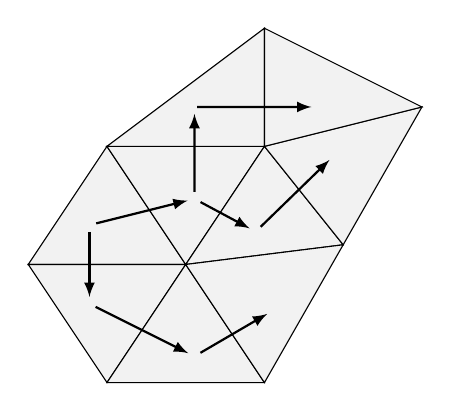
\begin{tikzpicture}
    \coordinate (A) at (0,0);
    \coordinate (B) at (2,0);
    \coordinate (C) at (1,1.5);
    \coordinate (D) at (3,1.5); 
    \coordinate (E) at (3,3); 
    \coordinate (F) at (4,0.25); 
    \coordinate (X) at (1,-1.5);
    \coordinate (Y) at (3,-1.5); 
    \coordinate (T) at (5,2); 
    
    \coordinate (CentroidABC) at ($(A)!0.3333!(B)!0.3333!(C)$);
    \coordinate (CentroidBCD) at ($(B)!0.3333!(C)!0.3333!(D)$);
    \coordinate (CentroidCDE) at ($(C)!0.3333!(D)!0.3333!(E)$);
    \coordinate (CentroidBDF) at ($(B)!0.3333!(D)!0.3333!(F)$);
    \coordinate (CentroidABX) at ($(A)!0.3333!(B)!0.3333!(X)$);
    \coordinate (CentroidBXY) at ($(Y)!0.3333!(B)!0.3333!(X)$);
    \coordinate (CentroidBFY) at ($(Y)!0.3333!(B)!0.3333!(F)$);
    \coordinate (CentroidDFT) at ($(D)!0.3333!(F)!0.3333!(T)$);
    \coordinate (CentroidDET) at ($(D)!0.3333!(E)!0.3333!(T)$);
    
    \draw[fill=gray!10] (A) -- (B) -- (C) -- cycle; 
    \draw[fill=gray!10] (B) -- (C) -- (D) -- cycle; 
    \draw[fill=gray!10] (C) -- (D) -- (E) -- cycle; 
    \draw[fill=gray!10] (B) -- (D) -- (F) -- cycle; 
    \draw[fill=gray!10] (A) -- (B) -- (X) -- cycle; 
    \draw[fill=gray!10] (Y) -- (B) -- (X) -- cycle; 
    \draw[fill=gray!10] (Y) -- (B) -- (F) -- cycle; 
    \draw[fill=gray!10] (T) -- (D) -- (F) -- cycle; 
    \draw[fill=gray!10] (T) -- (D) -- (E) -- cycle; 
    
    \draw[-latex, thick, shorten <=2.5pt, shorten >=2.5pt] (CentroidABC) -- (CentroidBCD); 
    \draw[-latex, thick, shorten <=2.5pt, shorten >=2.5pt] (CentroidBCD) -- (CentroidCDE); 
    \draw[-latex, thick, shorten <=2.5pt, shorten >=2.5pt] (CentroidBCD) -- (CentroidBDF); 
    \draw[-latex, thick, shorten <=2.5pt, shorten >=2.5pt] (CentroidABC) -- (CentroidABX); 
    \draw[-latex, thick, shorten <=2.5pt, shorten >=2.5pt] (CentroidABX) -- (CentroidBXY); 
    \draw[-latex, thick, shorten <=2.5pt, shorten >=2.5pt] (CentroidBXY) -- (CentroidBFY); 
    \draw[-latex, thick, shorten <=2.5pt, shorten >=2.5pt] (CentroidBDF) -- (CentroidDFT); 
    \draw[-latex, thick, shorten <=1.0pt, shorten >=2.0pt] (CentroidCDE) -- (CentroidDET); 
    
%     \node at (A) [below left] {$A$};
%     \node at (B) [below right] {$B$};
%     \node at (C) [above] {$C$};
%     \node at (D) [above right] {$D$};
%     \node at (T) [above right] {$T$};
\end{tikzpicture}
\end{center}
\caption{Strongly connected triangulation of a domain. The arrows depict a tree in the strong connection graph of the form used in Theorem~\ref{theorem:poincarefriedrichsestimate:grad}. The triangle in dark gray is the triangle being added in the current iteration, and the light gray triangles constitute the subdomain assembled so far.}
\end{figure}

%%%%%%%%%%%%%%%%%%%%%%%%%%%%%%%%%%%%%%%%%%%%%%%%%%%%%%%%%%%%%%%%%%%%%%%%%%%%%%%%%%%%%%%%%%%%%%%%%%%%%%%%%%%%%%%%%%%%%%%%
%%%%%%%%%%%%%%%%%%%%%%%%%%%%%%%%%%%%%%%%%%%%%%%%%%%%%%%%%%%%%%%%%%%%%%%%%%%%%%%%%%%%%%%%%%%%%%%%%%%%%%%%%%%%%%%%%%%%%%%%
%%%%%%%%%%%%%%%%%%%%%%%%%%%%%%%%%%%%%%%%%%%%%%%%%%%%%%%%%%%%%%%%%%%%%%%%%%%%%%%%%%%%%%%%%%%%%%%%%%%%%%%%%%%%%%%%%%%%%%%%
%%%%%%%%%%%%%%%%%%%%%%%%%%%%%%%%%%%%%%%%%%%%%%%%%%%%%%%%%%%%%%%%%%%%%%%%%%%%%%%%%%%%%%%%%%%%%%%%%%%%%%%%%%%%%%%%%%%%%%%%
%%%%%%%%%%%%%%%%%%%%%%%%%%%%%%%%%%%%%%%%%%%%%%%%%%%%%%%%%%%%%%%%%%%%%%%%%%%%%%%%%%%%%%%%%%%%%%%%%%%%%%%%%%%%%%%%%%%%%%%%
%%%%%%%%%%%%%%%%%%%%%%%%%%%%%%%%%%%%%%%%%%%%%%%%%%%%%%%%%%%%%%%%%%%%%%%%%%%%%%%%%%%%%%%%%%%%%%%%%%%%%%%%%%%%%%%%%%%%%%%%
%%%%%%%%%%%%%%%%%%%%%%%%%%%%%%%%%%%%%%%%%%%%%%%%%%%%%%%%%%%%%%%%%%%%%%%%%%%%%%%%%%%%%%%%%%%%%%%%%%%%%%%%%%%%%%%%%%%%%%%%
%%%%%%%%%%%%%%%%%%%%%%%%%%%%%%%%%%%%%%%%%%%%%%%%%%%%%%%%%%%%%%%%%%%%%%%%%%%%%%%%%%%%%%%%%%%%%%%%%%%%%%%%%%%%%%%%%%%%%%%%
%%%%%%%%%%%%%%%%%%%%%%%%%%%%%%%%%%%%%%%%%%%%%%%%%%%%%%%%%%%%%%%%%%%%%%%%%%%%%%%%%%%%%%%%%%%%%%%%%%%%%%%%%%%%%%%%%%%%%%%%
%%%%%%%%%%%%%%%%%%%%%%%%%%%%%%%%%%%%%%%%%%%%%%%%%%%%%%%%%%%%%%%%%%%%%%%%%%%%%%%%%%%%%%%%%%%%%%%%%%%%%%%%%%%%%%%%%%%%%%%%
%%%%%%%%%%%%%%%%%%%%%%%%%%%%%%%%%%%%%%%%%%%%%%%%%%%%%%%%%%%%%%%%%%%%%%%%%%%%%%%%%%%%%%%%%%%%%%%%%%%%%%%%%%%%%%%%%%%%%%%%
%%%%%%%%%%%%%%%%%%%%%%%%%%%%%%%%%%%%%%%%%%%%%%%%%%%%%%%%%%%%%%%%%%%%%%%%%%%%%%%%%%%%%%%%%%%%%%%%%%%%%%%%%%%%%%%%%%%%%%%%
%%%%%%%%%%%%%%%%%%%%%%%%%%%%%%%%%%%%%%%%%%%%%%%%%%%%%%%%%%%%%%%%%%%%%%%%%%%%%%%%%%%%%%%%%%%%%%%%%%%%%%%%%%%%%%%%%%%%%%%%
%%%%%%%%%%%%%%%%%%%%%%%%%%%%%%%%%%%%%%%%%%%%%%%%%%%%%%%%%%%%%%%%%%%%%%%%%%%%%%%%%%%%%%%%%%%%%%%%%%%%%%%%%%%%%%%%%%%%%%%%
%%%%%%%%%%%%%%%%%%%%%%%%%%%%%%%%%%%%%%%%%%%%%%%%%%%%%%%%%%%%%%%%%%%%%%%%%%%%%%%%%%%%%%%%%%%%%%%%%%%%%%%%%%%%%%%%%%%%%%%%
%%%%%%%%%%%%%%%%%%%%%%%%%%%%%%%%%%%%%%%%%%%%%%%%%%%%%%%%%%%%%%%%%%%%%%%%%%%%%%%%%%%%%%%%%%%%%%%%%%%%%%%%%%%%%%%%%%%%%%%%
%%%%%%%%%%%%%%%%%%%%%%%%%%%%%%%%%%%%%%%%%%%%%%%%%%%%%%%%%%%%%%%%%%%%%%%%%%%%%%%%%%%%%%%%%%%%%%%%%%%%%%%%%%%%%%%%%%%%%%%%
%%%%%%%%%%%%%%%%%%%%%%%%%%%%%%%%%%%%%%%%%%%%%%%%%%%%%%%%%%%%%%%%%%%%%%%%%%%%%%%%%%%%%%%%%%%%%%%%%%%%%%%%%%%%%%%%%%%%%%%%
%%%%%%%%%%%%%%%%%%%%%%%%%%%%%%%%%%%%%%%%%%%%%%%%%%%%%%%%%%%%%%%%%%%%%%%%%%%%%%%%%%%%%%%%%%%%%%%%%%%%%%%%%%%%%%%%%%%%%%%%
%%%%%%%%%%%%%%%%%%%%%%%%%%%%%%%%%%%%%%%%%%%%%%%%%%%%%%%%%%%%%%%%%%%%%%%%%%%%%%%%%%%%%%%%%%%%%%%%%%%%%%%%%%%%%%%%%%%%%%%%
%%%%%%%%%%%%%%%%%%%%%%%%%%%%%%%%%%%%%%%%%%%%%%%%%%%%%%%%%%%%%%%%%%%%%%%%%%%%%%%%%%%%%%%%%%%%%%%%%%%%%%%%%%%%%%%%%%%%%%%%
%%%%%%%%%%%%%%%%%%%%%%%%%%%%%%%%%%%%%%%%%%%%%%%%%%%%%%%%%%%%%%%%%%%%%%%%%%%%%%%%%%%%%%%%%%%%%%%%%%%%%%%%%%%%%%%%%%%%%%%%
%%%%%%%%%%%%%%%%%%%%%%%%%%%%%%%%%%%%%%%%%%%%%%%%%%%%%%%%%%%%%%%%%%%%%%%%%%%%%%%%%%%%%%%%%%%%%%%%%%%%%%%%%%%%%%%%%%%%%%%%
%%%%%%%%%%%%%%%%%%%%%%%%%%%%%%%%%%%%%%%%%%%%%%%%%%%%%%%%%%%%%%%%%%%%%%%%%%%%%%%%%%%%%%%%%%%%%%%%%%%%%%%%%%%%%%%%%%%%%%%%
%%%%%%%%%%%%%%%%%%%%%%%%%%%%%%%%%%%%%%%%%%%%%%%%%%%%%%%%%%%%%%%%%%%%%%%%%%%%%%%%%%%%%%%%%%%%%%%%%%%%%%%%%%%%%%%%%%%%%%%%
%%%%%%%%%%%%%%%%%%%%%%%%%%%%%%%%%%%%%%%%%%%%%%%%%%%%%%%%%%%%%%%%%%%%%%%%%%%%%%%%%%%%%%%%%%%%%%%%%%%%%%%%%%%%%%%%%%%%%%%%
%%%%%%%%%%%%%%%%%%%%%%%%%%%%%%%%%%%%%%%%%%%%%%%%%%%%%%%%%%%%%%%%%%%%%%%%%%%%%%%%%%%%%%%%%%%%%%%%%%%%%%%%%%%%%%%%%%%%%%%%
%%%%%%%%%%%%%%%%%%%%%%%%%%%%%%%%%%%%%%%%%%%%%%%%%%%%%%%%%%%%%%%%%%%%%%%%%%%%%%%%%%%%%%%%%%%%%%%%%%%%%%%%%%%%%%%%%%%%%%%%
%%%%%%%%%%%%%%%%%%%%%%%%%%%%%%%%%%%%%%%%%%%%%%%%%%%%%%%%%%%%%%%%%%%%%%%%%%%%%%%%%%%%%%%%%%%%%%%%%%%%%%%%%%%%%%%%%%%%%%%%
%%%%%%%%%%%%%%%%%%%%%%%%%%%%%%%%%%%%%%%%%%%%%%%%%%%%%%%%%%%%%%%%%%%%%%%%%%%%%%%%%%%%%%%%%%%%%%%%%%%%%%%%%%%%%%%%%%%%%%%%
%%%%%%%%%%%%%%%%%%%%%%%%%%%%%%%%%%%%%%%%%%%%%%%%%%%%%%%%%%%%%%%%%%%%%%%%%%%%%%%%%%%%%%%%%%%%%%%%%%%%%%%%%%%%%%%%%%%%%%%%
%%%%%%%%%%%%%%%%%%%%%%%%%%%%%%%%%%%%%%%%%%%%%%%%%%%%%%%%%%%%%%%%%%%%%%%%%%%%%%%%%%%%%%%%%%%%%%%%%%%%%%%%%%%%%%%%%%%%%%%%
%%%%%%%%%%%%%%%%%%%%%%%%%%%%%%%%%%%%%%%%%%%%%%%%%%%%%%%%%%%%%%%%%%%%%%%%%%%%%%%%%%%%%%%%%%%%%%%%%%%%%%%%%%%%%%%%%%%%%%%%
%%%%%%%%%%%%%%%%%%%%%%%%%%%%%%%%%%%%%%%%%%%%%%%%%%%%%%%%%%%%%%%%%%%%%%%%%%%%%%%%%%%%%%%%%%%%%%%%%%%%%%%%%%%%%%%%%%%%%%%%


\begin{figure}[t]
\begin{center}
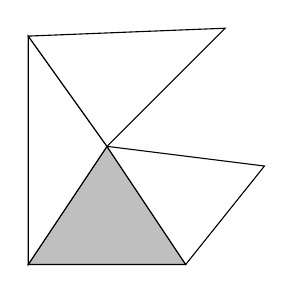
\begin{tikzpicture}
    \coordinate (A) at (0,0);   \coordinate (B) at (2,0); \coordinate (C) at (1,1.5);
    \coordinate (D) at (0,2.9); \coordinate (E) at (2.5,3); \coordinate (F) at (3,1.25); 
    \draw[fill=gray!50] (A) -- (B) -- (C) -- cycle; 
    \draw[fill=white  ] (A) -- (C) -- (D) -- cycle; 
    \draw[fill=white  ] (C) -- (D) -- (E) -- cycle; 
    \draw[fill=white  ] (B) -- (C) -- (F) -- cycle; 
\end{tikzpicture}
\quad
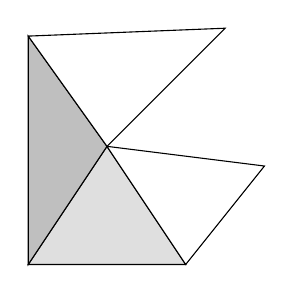
\begin{tikzpicture}
    \coordinate (A) at (0,0);   \coordinate (B) at (2,0); \coordinate (C) at (1,1.5);
    \coordinate (D) at (0,2.9); \coordinate (E) at (2.5,3); \coordinate (F) at (3,1.25); 
    \draw[fill=gray!25] (A) -- (B) -- (C) -- cycle; 
    \draw[fill=gray!50] (A) -- (C) -- (D) -- cycle; 
    \draw[fill=white  ] (C) -- (D) -- (E) -- cycle; 
    \draw[fill=white  ] (B) -- (C) -- (F) -- cycle; 
\end{tikzpicture}
\quad
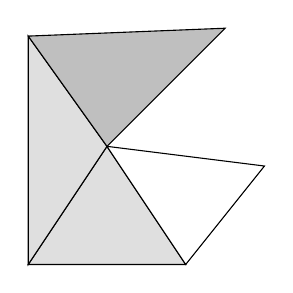
\begin{tikzpicture}
    \coordinate (A) at (0,0);   \coordinate (B) at (2,0); \coordinate (C) at (1,1.5);
    \coordinate (D) at (0,2.9); \coordinate (E) at (2.5,3); \coordinate (F) at (3,1.25); 
    \draw[fill=gray!25] (A) -- (B) -- (C) -- cycle; 
    \draw[fill=gray!25] (A) -- (C) -- (D) -- cycle; 
    \draw[fill=gray!50] (C) -- (D) -- (E) -- cycle; 
    \draw[fill=white  ] (B) -- (C) -- (F) -- cycle; 
\end{tikzpicture}
\quad
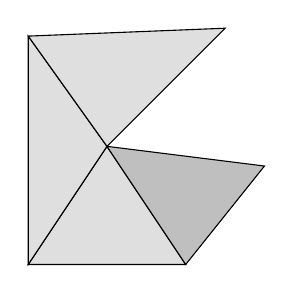
\begin{tikzpicture}
    \coordinate (A) at (0,0);   \coordinate (B) at (2,0); \coordinate (C) at (1,1.5);
    \coordinate (D) at (0,2.9); \coordinate (E) at (2.5,3); \coordinate (F) at (3,1.25); 
    \draw[fill=gray!25] (A) -- (B) -- (C) -- cycle; 
    \draw[fill=gray!25] (A) -- (C) -- (D) -- cycle; 
    \draw[fill=gray!25] (C) -- (D) -- (E) -- cycle; 
    \draw[fill=gray!50] (B) -- (C) -- (F) -- cycle; 
\end{tikzpicture}
\end{center}
\caption{Exhausting a domain step by step as in Theorem~\ref{theorem:poincarefriedrichsestimate:grad} and \ref{theorem:poincarefriedrichsestimate:gradzwei}.
The dark gray triangle is the one being currently added, and the light gray triangles constitute the subdomain assembled so far.}
\label{figure:exhausting}
\end{figure}



\begin{theorem}\label{theorem:poincarefriedrichsestimate:grad}
    Let $\Omega \subseteq \bbR^{n}$ be a domain with a strongly-connected finite triangulation $\calT$.
    Let $T_0 \in \calT$ be an $n$-simplex such that for all $n$-simplices $T \in \calT$ 
    we fix a strong path $T_0, T_1, \dots, T_m = T$.
    Suppose $1 \leq p,q \leq \infty$ with $1 = 1/p + 1/q$.
    Then for any $u \in W^{1,p}(\Omega)$ 
    there exists $w \in W^{1,p}(\Omega)$ with $\nabla u = \nabla w$ 
    and such that for all $T \in \calT$:
%     DONE {Make sure the notation for the PF constants is uniform throughout the paper}
    \begin{align*} 
        % \color{red}
        \| w \|_{L^{p}(T_m)}
        &\leq 
        \left( 1 + \volumeratio(\calT)^{\frac q p} \right)^{\frac 1 q}
        \sum_{t=1}^{m}
        \volumeratio(\calT)^{\frac{m-t}{p}}
        C_{{\rm{PF}},T_{t} \cup T_{t-1},p}
        % 2 C_{\PF,{\rm EFNT},p} \volumeratio(\calT)^{\frac 1 p} \max\left( \diam(T_{t}), \diam(T_{t-1}) \right)
        \| \nabla u \|_{L^{p}(T_{t} \cup T_{t-1})}
        \\&\quad \quad \quad 
        +
        \volumeratio(\calT)^{\frac{m-1}{p}}
        % C_{\PF,{\rm EFNT},p} \diam(T_0)
        C_{{\rm{PF}},T_{0},p}
        \| \nabla u \|_{L^{p}(T_{0})}
        .
    \end{align*}
    \todo{Rewrite this result.}
    When $1 < p < \infty$, letting $q := p/(p-1) \in (1,\infty)$ be the complementary exponent, we observe 
    \begin{align*}
        \| w_{m} \|_{L^{p}(T_m)}
        &\leq 
        \left( 1 + \frac{ \vol(T_m)^{\frac q p} }{ \vol(T_{{m-1}})^{\frac q p} } \right)^{\frac 1 q}
        \| w_{F_{m}} \|_{L^{p}(U_{F_m})} 
        +
        \frac{ \vol(T_m)^{\frac 1 p} }{ \vol(T_{{m-1}})^{\frac 1 p} }
        \| w_{m-1}\|_{L^{p}(T_{{m-1}})}
        .
    \end{align*}
\end{theorem}

\begin{proof}
 Let $u \in W^{1,p}(\Omega)$. 
 For each $F \in \calT$ of dimension $n-1$, 
 we let $w_F \in W^{1,p}(U_F)$ such that $\nabla w_F = \nabla u$ over $U_F$ and such that 
 \begin{align*}
    \| w_F \|_{L^{p}(U_F)} \leq C_{{\rm{PF}},U_F,p} \| \nabla w_F \|_{L^{p}(U_F)},
 \end{align*}
 where the computable constant $C_{{\rm{PF}},U_F,p}$ is determined via Lemma~\ref{lemma:poincarefriedrichsoverfacepatch}.
 We start with the simplex $T_{0}$. 
 There exists $w_0 \in W^{1,p}(T_{0})$ satisfying $\nabla w_0 = \nabla u$ over $T_{0}$ together with 
 \begin{gather*}
    \| w_0 \|_{L^{p}(T_{0})} \leq C_{{\rm{PF}},T_{0},p} \| \nabla u \|_{L^{p}(T_{0})}.
 \end{gather*}
 In particular, $c_{0} := u - w_0$ is a constant function. 
 
 Now, let $T \in \calT$ be any $n$-simplex. 
 By assumption, there exists a strong path $T_0, T_1, \dots, T_M = T$, composed of $n$-simplices. 
 We let $\Omega_m := \cup_{j=0}^{m} T_m$ for any $0 \leq m \leq M$,
 which is a triangulated $n$-dimensional submanifold with boundary.
 For any $1 \leq m \leq M$ we write $F_m := T_m \cap T_{m-1}$,
 which is a face of dimension $n-1$. 
 
%  Since $\calT$ is strongly connected, there exists an enumeration of $n$-simplices $T_0, T_1, \dots, T_M$ such that for any $1 \leq m \leq M$ there exists some fixed but arbitrary $0 \leq j(m) < m$ such that $F_m := T_m \cap T_{j(m)}$ is a face of dimension $n-1$. We write $\Omega_m := \cup_{j=0}^{m} T_m$. Hence $\Omega = \Omega_M$. 
 
 % DONE \notice{MWL, MV: add a figure here to illustrate how the domain is exhausted.}
 
 We construct the potential recursively. 
 We have seen that $c_{0} = w_{0} - u_{|\Omega_{0}}$ is a constant. 
 Assume that $1 \leq m \leq M$ such that there exists $w_{m-1} \in W^{1,p}(\Omega_{m-1})$ 
 such that $c_{0} = w_{m-1} - u_{|\Omega_{m-1}}$ is the constant above. 
 % Note that this assumption is already satisfied when $m=1$.
 Hence $\nabla w_{m-1} = \nabla u$ over $\Omega_{m-1}$. 
 By assumption, $T_{m}$ shares the face $F_{m}$ with $T_{{m-1}}$. 
 Since $$\nabla w_{F_{m}|T_{{m-1}}} = \nabla w_{m-1|T_{{m-1}}},$$
 there exists a constant $$c_{m} := w_{m-1|T_{{m-1}}} - w_{F_{m}|T_{{m-1}}}.$$
 We define $w'_{F_m} := w_{F_m} + c_{m} \in W^{1,p}(U_F)$.
 By construction, $$\nabla w'_{F_m} = \nabla w_{F_m} = \nabla u_{|U_{F_m}}$$ 
 and 
 $w'_{F_{m}|T_{{m-1}}} = w_{m-1|T_{{m-1}}}$. 
 But that already implies $w'_{F_m} = w_{|F_m} - c_{0}$. 
 Defining $w_{m} \in W^{1,p}(\Omega_m)$ by extending $w_{m-1}$ with $w'_{F_m|T_m}$,
 we have $c_{0} = w_{m} - u_{|\Omega_{m}}$. 
 
 We assess the norm of this potential. We observe 
 \begin{gather*}
    \| w_{m} \|_{L^{p}(T_m)}
    =
    \| w'_{F_m} \|_{L^{p}(T_m)}
    \leq 
    \| w_{F_m} \|_{L^{p}(T_m)}
    +
    \| c_{m} \|_{L^{p}(T_m)},
    \\
    \| c_{m} \|_{L^{p}(T_m)}
    = 
    \frac{ \vol(T_m)^{\frac 1 p} }{ \vol(T_{{m-1}})^{\frac 1 p} }
    \| c_{m} \|_{L^{p}(T_{{m-1}})},
    \\ 
    \| c_{m} \|_{L^{p}(T_{{m-1}})}
    \leq 
    \| w_{m-1}\|_{L^{p}(T_{{m-1}})} + \| w_{F_{m}} \|_{L^{p}(T_{{m-1}})} 
    .
 \end{gather*}
 In particular,
 \begin{align*}
    \| w_{m} \|_{L^{p}(T_m)}
    &
    \leq 
    \| w_{F_m} \|_{L^{p}(T_m)}
    \\&\qquad 
    +
    \frac{ \vol(T_m)^{\frac 1 p} }{ \vol(T_{{m-1}})^{\frac 1 p} }
    \| w_{F_{m}} \|_{L^{p}(T_{{m-1}})}
    +
    \frac{ \vol(T_m)^{\frac 1 p} }{ \vol(T_{{m-1}})^{\frac 1 p} }
    \| w_{m-1}\|_{L^{p}(T_{{m-1}})}
    .
 \end{align*}
 We sum the two integrals of $w_{F_m}$. 
 % 
 In the special case $p=1$,
 \begin{align*}
    \| w_{m} \|_{L^{1}(T_m)}
    \leq 
    \max\left(
        1, \frac{ \vol(T_m) }{ \vol(T_{{m-1}}) } 
    \right)
    \| w_{F_m} \|_{L^{1}(U_{F_m})}
    +
    \frac{ \vol(T_m) }{ \vol(T_{{m-1}}) }
    \| w_{m-1}\|_{L^{1}(T_{{m-1}})}
    .
 \end{align*}
 In the special case $p=\infty$, 
 \begin{align*}
    \| w_{m} \|_{L^{\infty}(T_m)}
    \leq 
    2
    \| w_{F_m} \|_{L^{\infty}(U_{F_m})}
    +
    \| w_{m-1}\|_{L^{\infty}(T_{{m-1}})}
    .
 \end{align*}
 % 1/q = 1 - 1/p = (p-1)/p 
 When $1 < p < \infty$, letting $q := p/(p-1) \in (1,\infty)$ be the complementary exponent, we observe 
 \begin{align*}
    \| w_{m} \|_{L^{p}(T_m)}
    &\leq 
    \left( 1 + \frac{ \vol(T_m)^{\frac q p} }{ \vol(T_{{m-1}})^{\frac q p} } \right)^{\frac 1 q}
    \left( 
        \| w_{F_{m}} \|_{L^{p}(T_m)}^{p}
        +
        \| w_{F_{m}} \|_{L^{p}(T_{{m-1}})}^{p}
    \right)^{\frac 1 p}
    \\&\qquad 
    +
    \frac{ \vol(T_m)^{\frac 1 p} }{ \vol(T_{{m-1}})^{\frac 1 p} }
    \| w_{m-1}\|_{L^{p}(T_{{m-1}})}
    \\&\leq 
    \left( 1 + \frac{ \vol(T_m)^{\frac q p} }{ \vol(T_{{m-1}})^{\frac q p} } \right)^{\frac 1 q}
    \| w_{F_{m}} \|_{L^{p}(U_{F_m})} 
    +
    \frac{ \vol(T_m)^{\frac 1 p} }{ \vol(T_{{m-1}})^{\frac 1 p} }
    \| w_{m-1}\|_{L^{p}(T_{{m-1}})}
    .
 \end{align*}
%  Recursive application provides the following estimate:
%  \begin{align*}
%     \| w_{m} \|_{L^{p}(T_m)}
%     &\leq 
%     \sum_{t=1}^{m} 
%     \left( 
%         \prod_{t < l \leq m} 
%         \frac{ \vol(T_l)^{\frac 1 p} }{ \vol(T_{l-1})^{\frac 1 p} } 
%     \right)
%     \left( 1 + \frac{ \vol(T_t)^{\frac q p} }{ \vol(T_{t-1})^{\frac q p} } \right)^{\frac 1 q}
%     \| w_{F_t} \|_{L^{p}(U_{F_t})}
%     \\&\quad \quad \quad 
%     +
%     \left( 
%         \prod_{0 < l \leq m} 
%         \frac{ \vol(T_l)^{\frac 1 p} }{ \vol(T_{l-1})^{\frac 1 p} } 
%     \right)
%     \| w_{T_0}\|_{L^{p}(T_{0})}
%     .
%  \end{align*}
%  We obtain the desired estimate. 
 % Taking into account Definition~\eqref{math:todo}, we obtain the desired inequality. % TODO: what was originally used here?
%  \begin{align*}
%     \| w_{m} \|_{L^{p}(T_m)}^{p}
%     &\leq 
%     (m+1)^{p-1}
%     % \sum_{t=1}^{m} \volumeratio(\calT)^{m-t} 
%     % \sum_{t=0}^{m-1} \volumeratio(\calT)^{t} 
%     \frac{\volumeratio(\calT)^{m}-1}{\volumeratio(\calT)-1}
%     \left( 1 + \volumeratio(\calT)^{\frac q p} \right)^{p/q}
%     \| w_{F_t} \|_{L^{p}(U_{F_t})}^{p}
%     \\&\quad \quad \quad 
%     +
%     (m+1)^{p-1}
%     \volumeratio(\calT)^{m-1}
%     \| w_{T_0}\|_{L^{p}(T_{0})}^{p}
%     .
%  \end{align*}
%  Notice that $p/q = p - 1$.
 % 
 Repeating this argument produces $w \in L^{p}(\Omega)$ 
 such that for all $n$-simplices $T \in \calT$ we have the restriction $w_{|T} \in W^{1,p}(T)$ with $w_{|T} = u + c_{0}$.
 In particular, $w \in W^{1,p}(\Omega)$ with $\nabla w = \nabla u$.
\end{proof}








\begin{lemma}\label{lemma:mixedbconsimplex}
    Let $T$ be an $n$-simplex with a face $F$. 
    If $u \in W^{1,p}(T)$ such that $\trace_{F} u = 0$, then 
    \begin{align*}
        \| u \|_{L^{p}(T)}
        &
        \leq 
        C_{\PF,T,F,p} \| \nabla u \|_{L^{p}(T)}
        ,
    \end{align*}
    where $C_{\PF,T,F,p} > 0$ is a constant such that 
    $C_{\PF,T,F,p} \leq \frac{1}{\sqrt[p]{p}} \diam(T)$.
%     \begin{align*}
%         C_{\PF,T,F,p}
%         &\leq 
%         C_{\PF,T,p} + \left( C_{\PF,T,p}^{p} + p \cdot \diam(T) C_{\PF,T,p}^{p-1} \right)^{\frac 1 p},  
%         \\
%         C_{\PF,T,F,p}
%         &\leq
%         \frac{1}{\sqrt[p]{p}}
%         \diam(T)
%         .
%     \end{align*}
\end{lemma}
\begin{proof}
\begin{comment}
    There exists $w \in W^{1,p}(T)$ with $\nabla w = \nabla u$ and 
    \begin{gather*}
        \| w \|_{L^{p}(T)}
        \leq 
        C_{\PF,T,p} 
        \| \nabla w \|_{L^{p}(T)} % DONE: bold face or no boldface? No bold face 
        .
    \end{gather*}
    Then $w-u$ is constant, and thus $\gamma := \trace_{F} (w-u) = \trace_{F} w$. 
    We use that 
    \begin{gather*}
        \| \gamma \|_{L^{p}(T)}
        =
        \gamma \vol(T)^\frac{1}{p}
        =
        \left( \frac{ \vol(T) }{ \vol(F) } \right)^\frac{1}{p}
        \cdot 
        \gamma 
        \vol(F)^\frac{1}{p}
        =
        \left( \frac{ \vol(T) }{ \vol(F) } \right)^\frac{1}{p}
        \| \gamma \|_{L^{p}(F)}
        .
    \end{gather*}
    Using a trace inequality~\cite[Lemma~2.8]{veeser2012poincare} when $1 \leq p < \infty$, we find 
    \begin{align*}
        \| \gamma \|_{L^{p}(F)}^{p}
        &
        \leq 
        \frac{ \vol(F) }{ \vol(T) }
        \| w \|_{L^{p}(T)}^{p}
        +
        p
        \cdot 
        \diam(T)
        \frac{ \vol(F) }{ \vol(T) }
        \| w \|_{L^{p}(T)}^{p-1}
        \| \nabla w \|_{L^{p}(T)}
        \\&
        \leq 
        \left( \frac{ \vol(F) }{ \vol(T) } \right)
        \left( C_{\PF,T,p}^{p} + p \cdot C_{\PF,T,p}^{p-1} \right) 
        \diam(T)^{p}
        \| \nabla w \|_{L^{p}(T)}^{p}
        \\&
        \leq 
        \left( \frac{ \vol(F) }{ \vol(T) } \right)
        \left( C_{\PF,T,p}^{p} + p \cdot \diam(T) C_{\PF,T,p}^{p-1} \right) 
        %\diam(T)^{p}
        \| \nabla w \|_{L^{p}(T)}^{p}
        .
    \end{align*}
    Recall that $u = w - \gamma$. The first inequality follows. 
\end{comment}
    % The second inequality follows from Rademacher's theorem when $p = \infty$.
    Since the inequality follows from Rademacher's theorem when $p = \infty$,
    we assume $1 \leq p < \infty$. 
    Let $u \in C^{\infty}(T)$ have support disjoint from $F$.
    Without loss of generality, 
    the segment from to the midpoint of $F$ to the opposing vertex lies on the first coordinate axis,
    and the minimal first coordinate among all the points of $F$ equals $0$. 
    We write $\bfg \in \bfL^{\infty}(\bbR^{n})$ for the trivial extension of $\nabla u$ outside of $T$.
    %With the fundamental theorem of calculus and H\"older's inequality: 
    We verify
    \begin{align*}
        \int_{T} |u(x)|^{p} \diff x \;dx
        &\leq
        \int_{\bbR^{n-1}} \int_{0}^{\diam(T)} |u( x_{1}, \overline x )|^{p} \;dx_{1} \;d\overline{x}
        \\&
        \leq
        \int_{\bbR^{n-1}} \int_{0}^{\diam(T)} \left| \int_{0}^{x_{1}} |\bfg( y, \overline x )| \,dy \right|^{p} \;dx_{1} \,d\overline{x}
        \\&
        \leq
        \int_{0}^{\diam(T)} x_{1}^{p-1} \int_{\bbR^{n-1}} \int_{0}^{x_{1}} \left| \bfg( y, \overline x ) \right|^{p} \;dy \,d\overline{x} \,dx_{1}
        \\&
        \leq
        \int_{0}^{\diam(T)} x_{1}^{p-1} \;dx_1 
        \cdot 
        \int_{T} \left| \bfg( y, \overline x ) \right|^{p} \;dy \,d\overline{x} 
        \leq
        \frac{\diam(T)^{p}}{p} \int_{T} \left| \nabla u( x ) \right|^{p} \,dx
        %
%         \leq
%         \int_{F} |u(x_{1},\dots,x_{n-1},x_{1})|^{p} \,dx_1 \dots \,dx_{n-1} \,dx_{1}
%         \\&
%         \leq
%         \int_{\Omega} \left| \int_{0}^{x_{1}} \partial_{n} u(x_{1},\dots,x_{n-1},y) \,dy \right|^{p} \,dx_1 \dots \,dx_{n-1} \,dx_{1}
%         \\&
%         \leq
%         \int_{\Omega} \int_{0}^{x_{1}} x_{1}^{p-1} \left| \partial_{n} u(x_{1},\dots,x_{n-1},y) \right|^{p} \,dy \,dx_1 \dots \,dx_{n-1} \,dx_{n}
%         \\&
%         \leq
%         \int_{\Omega} \int_{0}^{D} D^{p-1} \left| \bfg(x_{1},\dots,x_{n-1},y) \right|^{p} \,dy \,dx_1 \dots \,dx_{n-1} \,dx_{n}
%         \leq 
%         D^{p} 
%         \int_{\Omega} |\nabla u|^{p} \,dx
        .
    \end{align*}
    That $\|u\|_{L^{p}(T)} \leq \diam(T) p^{-\frac 1 p} \|\nabla u\|_{L^{p}(T)}$ 
    for all $W^{1,p}(T)$ whose members have vanishing trace along $F$ follows from approximation via members of $u \in C^{\infty}(T)$ whose support is disjoint from $F$. 
    
    Very briefly verify that density argument: 
    There exists $\varphi : \Delta^{n} \rightarrow T$ mapping the convex closure of the $n$ unit vectors onto the face $F$.
    We let $\hat u := u \circ \varphi$.
    Let $\hat U$ be the unit ball of the $\ell^1$ metric, which contains $\Delta^{n}$.
    We let $\tilde u$ be the extension of $\hat u$ onto $\hat U$ by reflection across the coordinate axes.
    Then $\tilde u \in W^{1,p}_{0}(\hat U)$, and $\tilde u$ is the limit of a sequence $u_{m} \in C^{\infty}_{c}(\hat U)$.
    Now $u_{m} \circ \varphi^{-1} \in C^{\infty}(\hat U)$ approximates $u$. 
\end{proof}

% \begin{remark}
%     While it may not be obvious, the second estimate is tighter than the first estimate when using the optimal Poincar\'e--Friedrichs constants for convex domains.  
% \end{remark}



















\begin{theorem}\label{theorem:poincarefriedrichsestimate:gradzwei}
    Let $\Omega \subseteq \bbR^{n}$ be a domain with a strongly connected finite triangulation $\calT$.
    Let $T_0 \in \calT$ be an $n$-simplex such that for all $n$-simplices $T \in \calT$ 
    we fix a strong path $T_0, T_1, \dots, T_m = T$.
    For any $1 \leq l \leq m$, let $F_{l} = T_{l} \cap T_{l-1}$.
    Then for any $u \in W^{1,p}(\Omega)$ 
    there exists $w \in W^{1,p}(\Omega)$ with $\nabla u = \nabla w$ 
    and such that for all $T \in \calT$:
    \begin{align*}
        \| w_{m} \|_{L^{p}(T_m)}
%         &\leq 
%         \volumeratio(\calT)^{\frac m p}
%         C_{\PF,T_{0},p} 
%         \| \nabla u \|_{L^{p}( T_{0} )}
%         +
%         \sum_{l=1}^{m} 
%         \volumeratio(\calT)^{\frac {m-l} p}
%         C_{\PF,T_{l},F_{l},p} 
%         \| \nabla u \|_{L^{p}(T_{l})} 
%         \\&\qquad 
%         +
%         \sum_{l=1}^{m} 
%         \volumeratio(\calT)^{\frac {m-l} p} \reflectionestimate(\calT)
%         C_{\PF,T_{l},F_{l},p} 
%         \| \nabla u \|_{L^{p}(T_{l-1})} 
%         \\
        &\leq 
        \volumeratio(\calT)^{\frac m p}
        C_{\PF,T_{0},p} 
        \| \nabla u \|_{L^{p}( T_{0} )}
        \\&\quad 
        +
        \sum_{l=1}^{m} 
        \volumeratio(\calT)^{\frac {m-l} p}
        C_{\PF,T_{l},F_{l},p} 
        \left( 
            \| \nabla u \|_{L^{p}(T_{l})} 
            +
            \volumeratio(\calT)^{\frac {1} p}
            \reflectionestimate(\calT)
            \| \nabla u \|_{L^{p}(T_{l-1})} 
        \right)
        .
    \end{align*}
%     \begin{align*}
%         \| w_{m} \|_{L^{p}(T_m)}
%         &\leq 
%         \sum_{l=1}^{m} 
%         \volumeratio(\calT)^{\frac{m-l}{p}}
%         \left( 1 + \volumeratio(\calT)^{\frac 1 p} \reflectionestimate(\calT) \right) 
%         C_{\PF,T_{l},F_{l},p} 
%         \| \nabla u \|_{L^{p}( T_{l} )}
%         +
%         \volumeratio(\calT)^{\frac m p}
%         C_{\PF,T_{0},p} 
%         \| \nabla u \|_{L^{p}( T_{0} )}
%         .
%     \end{align*}
%     \color{red}Precise form of the inequality yet to be discussed, though the construction principle is clear.
\end{theorem}

\begin{proof}
    Let $u \in W^{1,p}(\Omega)$. 
    First, there exists $w_0 \in W^{1,p}(T_{0})$ satisfying $\nabla w_0 = \nabla u$ over $T_{0}$ together with 
    \begin{gather*}
        \| w_0 \|_{L^{p}(T_{0})} \leq C_{{\rm{PF}},T_{0},p} \| \nabla u \|_{L^{p}(T_{0})}.
    \end{gather*}
    In particular, $c_{0} := u - w_0$ is a constant function. 

    Now, let $T \in \calT$ be any $n$-simplex. 
    By assumption, there exists a strong path $T_0, T_1, \dots, T_M = T$, composed of $n$-simplices. 
    For any $1 \leq m \leq M$ we let $F_m := T_m \cap T_{m-1}$ be a face of dimension $n-1$. 
    We write $\Omega_m := \cup_{j=0}^{m} T_m$, which is a triangulated $n$-dimensional submanifold with boundary.
    
    We use a recursive argument.
    Suppose that $0 < m \leq M$ such that there exists $w_{m-1} \in W^{1,p}(\Omega_{m-1})$ with $c_{0} = u - w_{m-1}$.
    In particular, $\nabla w_{m-1} = \nabla u$ over $\Omega_{m-1}$. 
    By assumption, $T_{m}$ shares the face $F_{m}$ with $T_{m-1}$. 
    % Let $\hat T$ be the reference simplex.
    % We fix affine diffeomorphisms $\varphi : \hat T \rightarrow T_{j(m)}$ and $\vartheta : \hat T \rightarrow T_{m+1}$,
    % each of which maps the convex closure of $v_0, \dots, v_{n-1}$ onto the common face $F_{m}$.
    %
    We define $w'_{m} := w_{m-1} \circ \Xi \in W^{1,p}(T_{m})$,
    where $\Xi : T_{m} \rightarrow T_{m-1}$ is the unique affine diffeomorphism that leaves $F_{m}$ invariant. 
    %
    By construction, $w'_{m} \in W^{1,p}(T_{m})$ with 
    \begin{align*}
        \trace_F w_{m-1} = \trace_F w'_{m}
        .
    \end{align*}
    %Write $w''_{m} = u - w'_{m} \in W^{1,p}(T_{m})$. Then 
    There exists $w''_{m} \in W^{1,p}(T_{m})$ such that 
    \begin{align*}
        \nabla w''_{m} = \nabla u_{|T_{m+1}} - \nabla w'_{m}, 
        \quad 
        \trace_{F_{m}} w''_{m} = 0.
    \end{align*}
    This is true because 
    \begin{align*}
        \trace_{F_{m}}( \nabla u - \nabla w'_{m} ) 
        &= 
        \trace_{F_{m}} \nabla u - \trace_{F_{m}} \nabla w'_{m}
        \\&= 
        \nabla \trace_{F_{m}} u - \nabla \trace_{F_{m}} w'_{m}
        = 
        \nabla \trace_{F_{m}} u - \nabla \trace_{F_{m}} w_{m-1}
        = 
        0
        .
    \end{align*}
    Setting $w_{m} := w_{m-1}$ over $\Omega_{m-1}$ and $w_{m} := w'_{m} + w''_{m}$ over $T_{m}$, 
    we find 
    \begin{gather*}
        \nabla w_{m} = \nabla w'_{m} + \nabla w''_{m} = \nabla w'_{m} + \nabla u - \nabla w'_{m} = \nabla u,
        % \end{gather*}
        \\
        % \begin{gather*}
        \trace_{F_{m}} w_{m} = \trace_{F_{m}} w'_{m} = \trace_{F_{m}} w_{m-1}.
    \end{gather*}
    That means that $w_{m} \in W^{1,p}(\Omega_{m})$ with $\nabla w_{m} = \nabla u$ over $\Omega_{m}$. 
    In particular, $c_{0} = u - w_{m}$. 
    Lemma~\ref{lemma:mixedbconsimplex} gives 
    \begin{align*}
        \| w''_{m} \|_{L^{p}(T_{m})} 
        &
        \leq 
        C_{\PF,T_{m},F_{m},p} \| \nabla u - \nabla w'_{m} \|_{L^{p}(T_{m})}.
        \\&
        \leq 
        C_{\PF,T_{m},F_{m},p} \| \nabla u      \|_{L^{p}(T_{m})} 
        + 
        C_{\PF,T_{m},F_{m},p} \| \nabla w'_{m} \|_{L^{p}(T_{m})} 
        .
    \end{align*}
    We also employ Lemma~\ref{lemma:volumecomparison} to find 
    \begin{align*}
        \| \nabla w'_{m} \|_{L^{p}(T_{m})}
        &
        \leq 
        |\det(\Jacobian \Xi  )|^{-\frac 1 p} 
        \| \Jacobian \Xi   \|
        \cdot 
        \| \nabla w_{m-1} \|_{L^{p}(T_{m-1})}
        \\&
        \leq 
        \volumeratio(\calT)^{\frac 1 p} \reflectionestimate(\calT)
        \cdot 
        \| \nabla w_{m-1} \|_{L^{p}(T_{m-1})}
        .
    \end{align*}
    Putting this all together, we use 
    \begin{align*}
        &
        \| w_{m} \|_{L^{p}(T_{m})}
        \\&
        \leq  
        \| w'_{m} \|_{L^{p}(T_{m})}
        + 
        \| w''_{m} \|_{L^{p}(T_{m})}
        \\&
        \leq  
        \volumeratio(\calT)^{\frac 1 p} 
        \| w_{m-1} \|_{L^{p}(T_{m-1})} 
        + 
        C_{\PF,T_{m},F_{m},p} 
        \left( 
            \| \nabla u \|_{L^{p}(T_{m})} 
            + 
            \| \nabla w'_{m} \|_{L^{p}(T_{m})} 
        \right) 
    \end{align*}
    and 
    \begin{align*}
        \| \nabla w'_{m} \|_{L^{p}(T_{m})} 
        &
        \leq  
        \volumeratio(\calT)^{\frac 1 p} \reflectionestimate(\calT)
        % C_{\PF,T_{m},F_{m},p} 
        \| \nabla w_{m-1} \|_{L^{p}(T_{m-1})} 
        \leq  
        \volumeratio(\calT)^{\frac 1 p} \reflectionestimate(\calT)
        % C_{\PF,T_{m},F_{m},p} 
        \| \nabla u \|_{L^{p}(T_{m-1})} 
%         \\&
%         \leq  
%         \volumeratio(\calT)^{\frac 1 p} 
%         \| w_{m-1} \|_{L^{p}(T_{m-1})} 
%         + 
%         \left( 1 + \volumeratio(\calT)^{\frac 1 p} \reflectionestimate(\calT) \right) 
%         C_{\PF,T_{m},F_{m},p} 
%         \| \nabla u \|_{L^{p}(T_{m})} 
        .
    \end{align*}
%     \begin{align*}
%         &
%         \| w_{m} \|_{L^{p}(T_{m})}
%         \\&
%         \leq  
%         \| w'_{m} \|_{L^{p}(T_{m})}
%         + 
%         \| w''_{m} \|_{L^{p}(T_{m})}
%         \\&
%         \leq  
%         \volumeratio(\calT)^{\frac 1 p} 
%         \| w_{m-1} \|_{L^{p}(T_{m-1})} 
%         + 
%         C_{\PF,T_{m},F_{m},p} 
%         \left( 
%             \| \nabla u \|_{L^{p}(T_{m})} 
%             + 
%             \| \nabla w'_{m} \|_{L^{p}(T_{m})} 
%         \right) 
%         \\&
%         \leq  
%         \volumeratio(\calT)^{\frac 1 p} 
%         \| w_{m-1} \|_{L^{p}(T_{m-1})} 
%         + 
%         C_{\PF,T_{m},F_{m},p} 
%         \| \nabla u \|_{L^{p}(T_{m})} 
%         + 
%         C_{\PF,T_{m},F_{m},p} 
%         \| \nabla w'_{m} \|_{L^{p}(T_{m})} 
%         \\&
%         \leq  
%         \volumeratio(\calT)^{\frac 1 p} 
%         \| w_{m-1} \|_{L^{p}(T_{m-1})} 
%         + 
%         C_{\PF,T_{m},F_{m},p} 
%         \| \nabla u \|_{L^{p}(T_{m})} 
%         + 
%         \volumeratio(\calT)^{\frac 1 p} \reflectionestimate(\calT)
%         C_{\PF,T_{m},F_{m},p} 
%         \| \nabla w_{m-1} \|_{L^{p}(T_{m-1})} 
%         \\&
%         \leq  
%         \volumeratio(\calT)^{\frac 1 p} 
%         \| w_{m-1} \|_{L^{p}(T_{m-1})} 
%         + 
%         C_{\PF,T_{m},F_{m},p} 
%         \| \nabla u \|_{L^{p}(T_{m})} 
%         + 
%         \volumeratio(\calT)^{\frac 1 p} \reflectionestimate(\calT)
%         C_{\PF,T_{m},F_{m},p} 
%         \| \nabla u \|_{L^{p}(T_{m-1})} 
%         \\&
%         \leq  
%         \volumeratio(\calT)^{\frac 1 p} 
%         \| w_{m-1} \|_{L^{p}(T_{m-1})} 
%         + 
%         \left( 1 + \volumeratio(\calT)^{\frac 1 p} \reflectionestimate(\calT) \right) 
%         C_{\PF,T_{m},F_{m},p} 
%         \| \nabla u \|_{L^{p}(T_{m})} 
%         .
%     \end{align*}
    The existence of $w \in W^{1,p}(\Omega)$ satisfying the recursive estimate follows. 
\end{proof}

\begin{remark}
    The previous theorems, Theorem~\ref{theorem:poincarefriedrichsestimate:grad} and Theorem~\ref{theorem:poincarefriedrichsestimate:gradzwei} 
    depend on only a few parameters of the triangulation:
    the length of any traversal from the root simplex, the ratios of the volumes of adjacent simplices,
    the Poincar\'e--Friedrichs constants on each face patch, and the Poincar\'e--Friedrichs constant of the initial simplex. 
    The aforementioned local Poincar\'e--Friedrichs constants can generally be estimated in terms of shape-parameters. 
    If the face patches of the triangulation are convex, then better estimates are possible. 
\end{remark}

% https://people.tamu.edu/~guermond//PUBLICATIONS/ern_guermond_m2an_2016.pdf 
% Lemma 5.5
























\section{Shellable triangulations of manifolds}\label{section:advancedtriangulations}

We return to the theory of triangulations,
as our main objective requires some further concepts.
We are interested in simplicial complexes that triangulate manifolds. 
Our particular interest are manifold triangulations that are \emph{shellable}.
Such simplicial complexes are constructed by successively adding simplices in a particularly well-behaved manner. 
\cye{Local} patches \cye{(stars)} within triangulations of dimension two and three are examples of such shellable complexes. 
The monographs by Kozlov~\cite{kozlov2008combinatorial} and Ziegler~\cite{ziegler1995lectures} are our main references for this section. 
We also refer to Lee's monograph~\cite{lee2011topological} for any further background on manifolds. 

\begin{figure}[h]
\centerline{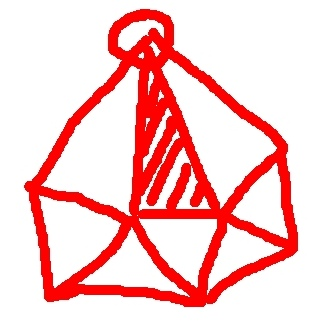
\includegraphics[width=0.2\textwidth]{homotopic_ball.jpg} \quad 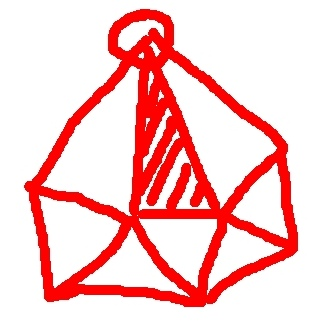
\includegraphics[width=0.2\textwidth]{homotopic_ball.jpg}}
\label{figure:not_manifold_triang}
\caption{A manifold triangulation (left) and not a manifold triangulation (right)}
\end{figure}


\subsection{Triangulations of manifolds}

We define an $n$-dimensional simplicial complex to be a \emph{manifold triangulation} if the underlying set $\underlying{\calT}$ is an $n$-dimensional manifold with boundary.
We recall that this means that for every $x \in \underlying{\calT}$
% there exists $\epsilon > 0$ and an embedding $\phi : \Ball_\epsilon(x) \cap \underlying{\calT} \rightarrow \bbR^{n}$
there exists an open neighborhood $U(x) \subseteq \underlying{\calT}$ and an embedding $\phi : U(x) \rightarrow \bbR^{n}$
such that $\phi(0) = 0$ and $\phi$ is an isomorphism either onto the open unit ball $\calB = \{ x \in \bbR^{n} \suchthat |x| < 1 \}$
or onto the half-ball $\{ x \in \calB \suchthat x_1 \geq 0 \}$.
In the former case, $x$ is called an \emph{interior point}, and in the latter case $x$ is called a \emph{boundary point}. 
Any simplicial complex that triangulates an $n$-dimensional manifold must be $n$-dimensional. 
\cye{An example of a manifold triangulation and an example which is not a manifold triangulation are given in Figure~\ref{figure:not_manifold_triang}.}

The following special cases receive particular interest:
an \textit{$n$-ball triangulation} is any triangulation of a topological (closed) $n$-ball\cye{\sout{,
and we sometimes call this a \textit{$n$-disk} triangulation}}.
An \textit{$n$-sphere triangulation} is any triangulation of a topological $n$-sphere. 


We know that any manifold $\calM$ has got a topological boundary $\partial\calM$, possibly empty. 
If $\calM$ is $n$-dimensional, then the $\partial\calM$ is a topological manifold without boundary of dimension $n-1$. 
We gather a few helpful observations on how these notions relate to triangulations.
While the reader might deem them obvious, we nevertheless include proofs. 

\begin{lemma}\label{lemma:boundarysimplices}
    Let $\calT$ be a finite $n$-dimensional simplicial complex whose underlying set is a manifold $\calM$. 
    \begin{itemize}
        \item Any face $F \in \Faces(\calT)$ is not contained in the boundary if and only if it is contained in exactly two $n$-simplices.
        \item Any face $F \in \Faces(\calT)$ is contained in the boundary if and only if it is contained in exactly one $n$-simplex.
        \item The simplices contained in the boundary constitute a triangulation of the boundary.
        % \item $\calT$ is non-branching, that is, every $F \in \calT$ of dimension $n-1$ is contained in at most two $n$-simplices of $\calT$. 
    \end{itemize}
\end{lemma}
\begin{proof}
    We prove these statements in several steps.
    \begin{enumerate}
    \item 
    Let $\mathring \calM := \calM \setminus \partial \calM$ denote the interior of the manifold. 
    We will use the following fact:\footnote{To see this, one easily constructs a continuous deformation of $\calM$ into itself to move any chosen point on $S$ to any other chosen point on $S$.} if $S \in \calT$ has an inner point that lies on $\partial \calM$, then all inner points of $S$ are on $\partial \calM$. 
    Since the boundary $\partial \calM$ is closed, every $S \in \calT$ is either a subset of the boundary or all its inner points lie in the interior $\mathring \calM$ of the manifold. 
    
    \item 
    We recall an auxiliary result.
    Suppose that $Y$ is a topological space homeomorphic to a sphere of dimension $m$ and that $X \subseteq Y$ is homeomorphic to a sphere of dimension $m-1$, where $m \geq 1$. 
    As a consequence of the Jordan--Brouwer separation theorem~\cite[Corollary IV.5.24]{mayer1989algebraische}~\cite[Corollary VIII.6.4]{massey1981algebraic}, 
    we know that $Y \setminus X$ has got two connected components.
    
    % \item 
    % We prove an auxiliary result. 
    % Suppose that $Y$ is a topological space homeomorphic to a sphere of dimension $m$ and that $X \subseteq Y$ is homeomorphic to a sphere of dimension $m-1$, where $m \geq 1$. 
    % The embedding of $X$ into $Y$ cannot be onto~\cite[Theorem~2.55]{lee2011topological}, and so there exists $y \in Y \setminus X$. 
    % Using the homeomorphism from $Y$ into the $m$-sphere, which maps $y$ to the northpole without loss of generality, and a stereographic projection, 
    % we see that $Y \setminus \{y\}$ is homeomorphic to $R^{m}$.
    % As a consequence of the Jordan--Brouwer separation theorem~\cite[Theorem IV.5.23]{mayer1989algebraische}~\cite[Corollary IV.5.24]{mayer1989algebraische}~\cite[Corollary VIII.6.4]{massey1981algebraic}, $Y \setminus (X \cup \{y\})$ has got two connected components,
    % and thus $Y \setminus X$ has got two connected components.
    
    \item
    Let $F \in \Faces(T)$ and let $z_F \in F$ be its barycenter. 
    Since $\calT$ is finite, we let $\mathring B_F$ be an open neighborhood around $z_F$ so small that it only intersects those $n$-simplices of $\calT$ that already contain $z_F$ and no faces other than $F$.
    Suppose there are distinct $n$-simplices $T_1, T_2, \dots, T_K$ that contain $z_F$. 
    The intersection of any two of them is $F$, but their interiors are disjoint because otherwise they would coincide. 
    
    If $z_F$ is an interior point of $\calM$, 
    then it follows by our assumptions that $\mathring B_F$ is homeomorphic to an open $n$-ball and $\partial \mathring B_F$ is homeomorphic to a sphere of dimension $n-1$. 
    Consider $X = F \cap \partial \mathring B_F$.
    If $n=1$, then $X$ is empty and $\partial \mathring B_F$ has $K$ distinct connected components. 
    If $n > 1$, then $X$ is homeomorphic to a sphere of dimension $n-2$
    and again $\partial \mathring B_F \setminus X$ has $K$ distinct connected components. 
    But by the auxiliary result above, $K = 2$. 
    We conclude that $F$ is contained in two $n$-simplices of $\calT$.
    
    Consider the case that $z_F$ lies on the boundary of $\calM$ and suppose that $F$ is contained in $K$ distinct $n$-simplices of $\calT$.
    By adding at least one dimension, we can double\footnote{The reader is referred to Lee's textbook~\cite{lee2012smooth} for more background and the technicalities.} the manifold $\calM$ along the boundary and obtain the doubled manifold $\calM'$. 
    Similarly, we can construct a doubling of the triangulation $\calT'$ such that $F$ is contained in exactly $2K$ distinct $n$-simplices of $\calT'$. 
    We know that $\calM'$ is a manifold without boundary, and hence $F$ is an interior simplex of $\calT'$.
    This implies $K=1$.
    So any boundary face can only be contained in one single $n$-simplex. 
    
    \item
    Clearly, the simplices of $\calT$ contained in the boundary constitute a simplicial complex. 
    Every $x \in \calM$ is an inner point of some simplex $S \in \calT$. 
    If $x \in \partial \calM$ is a boundary point, then $S$ must be a boundary simplex, 
    so the boundary simplices triangulate all of $\partial \calM$.
    \end{enumerate}
    All desired results are thus proven. 
\end{proof}

Suppose that $\calT$ is an $n$-dimensional simplicial complex that triangulates a manifold. 
Those simplices of the manifold triangulation that are subsets of the boundary of the underlying manifold are called \emph{boundary simplices}. 
% The simplices that lie in the boundary of the underlying set are called \emph{boundary simplices}.
All other simplices of the manifold triangulation are called \emph{inner simplices}. 
We have seen that the boundary simplices of a manifold triangulation constitute a triangulation of the manifolds boundary. 
We call this simplicial complex the \emph{boundary complex}. It has dimension $n-1$. 
% We see that the family of boundary faces constitute a simplicial complex, which we call \textit{boundary complex}.
% Any point on the boundary lies within some boundary simplex, and hence the boundary complex is a triangulation of the boundary. 
% Definitions imply that the boundary complex is a manifold triangulation of dimension $n-1$.
% The boundary simplices of a manifold triangulation of dimension $n$ constitute a manifold triangulation themselves, of dimension $n-1$, which triangulate the boundary of the underlying space. 

We continue with a few more observations about manifold triangulations
at the intersection of topology and combinatorics. 
These include the topology of local patches (stars), which is a surprisingly non-trivial topic. 
We say that an $n$-dimensional manifold triangulation $\calT$ is \emph{locally vertex combinatorial}
if the star of every simplex $S \in \calT$ is a triangulated $n$-dimensional ball that contains $S$.
We gather some results that are hard to find in the literature. 

\begin{lemma}\label{lemma:startopology}
    Let $\calT$ be a finite $n$-dimensional simplicial complex whose underlying space is a manifold $\calM$.
    Suppose that $1 \leq n \leq 3$. Then the following holds:
    \begin{itemize}
        \item
        If $S \in \calT$ is an inner simplex, 
        then $\patch_{\calT}(S)$ is a simplicial $n$-ball with $S$ as an inner simplex
        and $\carapace_{\calT}(S)$ is a simplicial $(n-1)$-sphere. 
        \item
        If $S \in \calT$ is a boundary subsimplex, 
        then $\patch_{\calT}(S)$ is a simplicial $n$-ball with $S$ as a boundary simplex,
        and $\carapace_{\calT}(S)$ is a simplicial $(n-1)$-ball.
    \end{itemize}
\end{lemma}
\begin{proof}
    The lemma is obvious if $n = 1$, so we assume $n \geq 2$ in what follows. 
    We prove these statements in several steps. 
    The reader is assumed to have some background in topology. 
    \begin{enumerate}
    \item 
    Let $S$ be any simplex with vertices $v_0, v_1, \dots, v_k$, with barycenter $z_{\cye{S}}$\todo{MV: OK?}, and dimension $k$.
    Let $\calS := \patch_{\calT}(S)$ be its star. 
    Each $l$-dimensional simplex $T \in \calS$ that contains $S$ 
    has vertices $v_0, v_1, \dots, v_k, v_{k+1}^{S}, \dots, v_{l}^{S}$. 
    For any such simplex, we introduce a decomposition $T_{0}, \dots, T_{k}$, where each $T_{i}$ has vertices 
    \begin{align*}
        v_0, \dots, v_{i-1}, z_{\cye{S}}, v_{i+1}, \dots, v_k, v_{k+1}^{S}, \dots, v_{l}^{S}.
    \end{align*}
    The collection $\calS'$ of these simplices and their subsimplices constitute a simplicial complex 
    that triangulates the same underlying set as $\calS$.
    Moreover, $\calS' = \patch_{\calS'}(z_{\cye{S}})$. 
    In particular, $z_{\cye{S}}$ is a boundary vertex of $\calS'$ if and only if $S$ is a boundary simplex of $\calS$. 
    So it remains to study the topology of vertex stars. 
    
    \item 
    Suppose that $2 \leq n \leq 3$ and that $\calM$ is a manifold without boundary. 
    Under these assumptions, 
    as explained in the proof of Theorem~1 in \cite{Siebenmann1979},
    the set $\carapace(V)$ is a triangulation of a sphere of dimension $n-1$ for any inner vertex $V$. 
    There exists a homeomorphism from the closed cone of $\underlying{\carapace(V)}$ onto the local star $\underlying{\patch_{\calT}(V)}$.
    But then that closed cone and hence $\underlying{\patch_{\calT}(V)}$ are homeomorphic to an $n$-dimensional ball. 
    
    \item 
    If $2 \leq n \leq 3$ and $\calM$ has a non-empty boundary, then we use an approach as in the proof of Lemma~\ref{lemma:boundarysimplices}: 
    we let $\calM'$ denote the doubling of the manifold and $\calT'$ be the doubling of the triangulation $\calT$. 
    Let $V \in \calT$ be a vertex. 
    If $V$ is an inner vertex of $\calT$, then $\carapace(V) \subseteq \calT \subseteq \calT'$ triangulates a sphere of dimension $n-1$ and $\patch_{\calT}(V) \subseteq \calT \subseteq \calT'$ triangulates a ball of dimension $n$, as discussed above. 
    If $V$ is a boundary vertex of $\calT$, then it is an inner vertex of $\calT'$,
    and so $\carapace_{\calT}(V) \subseteq \calT'$ triangulates a sphere of dimension $n-1$ and $\patch_{\calT}(V) \subseteq \calT'$ triangulates a ball of dimension $n$.
    We also know that $\carapace_{\partial\calT}(V) \subseteq \partial\calT$ triangulates a sphere of dimension $n-2$ and $\patch_{\partial\calT}(V) \subseteq \partial\calT$ triangulates a ball of dimension $n-1$. 
    The embedding of $\carapace_{\partial\calT}(V) \subseteq \partial\calT$ is homeomorphic to the standard embedding of the $(n-2)$-dimensional unit sphere into the $(n-1)$-dimensional unit sphere. 
    It follows that $\carapace_{\calT}(V)$ triangulates a topological ball of dimension $n-1$.
    Since the closed cone of $\underlying{\carapace(V)}$ is homeomorphic to the star $\underlying{\patch_{\calT}(V)}$, we conclude that $\patch_{\calT}(V)$ triangulates an $n$-dimensional ball. 
    
    
%     Suppose that $S = \{z\}$ is a singleton simplex. 
%     For $\delta > 0$ small enough, 
%     \begin{align*}
%         B_{\delta}(z) = \left\{ x \in \calM \suchthat d(x,z) \leq \delta \right\},
%         \quad 
%         S_{\delta}(z) = \left\{ x \in \calM \suchthat d(x,z) = \delta \right\},
%     \end{align*}
%     are compactly contained subsets of $|\patch_{\calT}(S)|$.
%     For each simplex $K \in \patch_{\calT}(S)$ that contains the vertex $z$ and which has the opposite face $F_K$, 
%     we easily find homeomorphisms $\phi_{K} : B_{\delta}(z) \cap K \rightarrow K$
%     such that 
%     $\phi_{K}(z) = z$, 
%     such that 
%     $\phi_{K}( K \cap S_{\delta}(z) ) = F_{K}$,
%     such that 
%     for all $K, K' \in \calT$ with $K' \subseteq K$ we have $\phi_{K|K'} = \phi_{K'}$,
%     and such that 
%     $\phi_{K}$ maps $[0,1]\cdot v$ linearly into $\bbR \cdot v$. 
%     This is defines a homeomorphism $\phi : B_{\delta}(z) \rightarrow |\patch_{\calT}(S)|$. 
%     Moreover, one easily verifies that $\phi$ is bi-Lipschitz.
%     %     For $\delta > 0$ small enough, $B_{\delta}(z)$ is homeomorphic to the unit ball and that homeomorphism maps $S_{\delta}(z)$ onto the unit sphere. 
%     \item 
%     One sees that $\phi$ defines a mapping from the closed 
%     homeomorphism between cone of link and ball 
%     
%     If $z$ is an inner vertex of $\calS'$, 
%     then the boundary simplices of $\calS'$,
%     which are the boundary simplices of $\calS$, triangulate a topological sphere of dimension $n-1$.
%     
%     Now suppose that $z$ is a boundary vertex of $\calS'$,
%     which is the case if and only if $S$ is a boundary simplex. 
%     Write 
%     \[
%         B_{H} = \left\{ x \in B_1(0) \suchthat* x_1 \leq 0 \right\},
%         \quad 
%         S_{H} = \left\{ x \in \partial B_1(0) \suchthat* x_1 \leq 0 \right\}.
%         \quad 
%         D_{H} = \left\{ x \in \partial B_1(0) \suchthat* x_1 = 0 \right\}.
%     \]
%     Provided that $\delta > 0$ is small enough, there exists a homeomorphism $\phi'$ that maps $\overline{B_{\delta}(z)} \cap \calM$ onto $B_1(0)$, which maps $\overline{B_{\delta}(z)} \cap \partial\calM$ onto $D_H$,
%     and which maps $z$ to the origin. 
%         %
%     It follows that $\phi'$ maps the closure of $\partial{B_{\delta}(z)} \setminus \partial\calM$ onto $S_H$.
%         %
%     Assuming that $\delta$ is small enough once more, 
%     we now verify that $\phi^{-1}$ maps $|\carapace(S)|$ onto $S_{\delta}(z) \cap |\patch_{\calT}(S)|$.
%     The latter equals the closure of $\partial{B_{\delta}(z)} \setminus \partial\calM$.
%     It follows that $\carapace(S)$ triangulates a topological ball of dimension $n-1$. 
    % We let $\calM'$ be the doubling of the manifold and let $\calT'$ be the doubling of the present triangulation;
    % we refer to Lee's textbook~\cite{lee2011topological} for details. 
    % The vertex star around $z$ within the boundary triangulation $\partial\calT$ is homeomorphic to the ball of dimension $n-1$,
    % and it is homeomorphic to $\overline{ B_{\delta}(z) } \cap |\partial\patch_{\calT}(S)|$ along $\phi$. 
    % The underlying space of $\carapace(S)$ is homeomorphic to $S_{\delta}(z) \cap |\patch_{\calT}(S)|$ along $\phi$.
    % The vertex star around $z$ within the boundary triangulation $\partial\calT$ is homeomorphic to the ball of dimension $n-1$,
    % and it is homeomorphic to $\overline{ B_{\delta}(z) } \cap |\partial\patch_{\calT}(S)|$ along $\phi$. 
    % Notice that 
    % \begin{align*}
    %     \partial\left( { B_{\delta}(z) } \cap |\partial\patch_{\calT}(S)| \right)
    %     =
    %     S_{\delta}(z) \cap |\patch_{\calT}(S)|
    %     \cup 
    %     \overline{ B_{\delta}(z) } \cap |\partial\patch_{\calT}(S)|
    %     .
    % \end{align*}
    % Necessarily, this homeomorphism maps the boundary of $\overline{B_{\delta}(z)} \cap |\calT|$, which contains $z$, onto the unit sphere. Since the image of $\overline{ B_{\delta}(z) } \cap |\partial\patch_{\calT}(S)|$ along $\phi'$ is still homeomorphic to a disk of dimension $n-1$, so must be the image of $S_{\delta}(z) \cap |\patch_{\calT}(S)|$ under $\phi'$.
    % But that just means that $\carapace(S)$ triangulates a topological ball of dimension $n-1$. 
    \end{enumerate}
    All relevant results are proven. 
\end{proof}


\begin{lemma}\label{lemma:connectivity}
    Let $\calT$ be a finite $n$-dimensional simplicial complex whose underlying space is a manifold $\calM$.
    If the underlying space of $\calT$ is connected, then $\calT$ is \cye{face} connected. \mwl{TODO Add a hyphen to each such instance.}
\end{lemma}
\begin{proof}
    We first show that each vertex star is \cye{face} connected via a short induction argument.
    Clearly, any simplicial $1$-ball and simplicial $1$-sphere are \cye{face} connected. 
    Now, if $n \geq 1$, then any vertex star in any $(n+1)$-dimensional manifold triangulation is already \cye{face} connected if all simplicial $n$-balls and $n$-spheres are \cye{face} connected.
    The induction argument implies that each vertex star in $\calT$ is \cye{face} connected.

    If the underlying space $\underlying{\calT}$ is connected, 
    then we easily see that the union of the $1$-simplices is path-connected.
    Given $n$-simplices $S,S' \in \calT$, 
    we can thus choose a sequence of $\hat S_0=S,\hat S_1,\dots,\hat S_m=S' \in \calT$ such that $\hat S_{i} \cap \hat S_{i-1} \neq \emptyset$ for all $1 \leq i \leq m$, and so each two consecutive simplices in that sequence have at least one vertex in common. 
    As each vertex star is \cye{face} connected, 
    we can thus assume without loss of generality that the sequence $S_0=S,S_1,\dots,S'=S_m \in \calT$ 
    is such that $S_{i} \cap S_{i-1}$ is a face of both $S_{i}$ and $S_{i-1}$ for all $1 \leq i \leq m$.
    This just means that $\calT$ is \cye{face} connected. 
\end{proof}



\begin{remark}
    Triangulations with the property that all vertex stars are homeomorphic to a ball are also called \emph{combinatorial} \cite[Section~1]{Bagchi2005}.
    All manifolds of dimension up to three admit smooth structures and smooth manifolds admit combinatorial triangulations. 
    There are triangulations of manifolds in dimension higher than $3$ where not every vertex star is homeomorphic to a ball. 
    
    Clearly, not every simplicial complex is the triangulation of some (embedded) topological manifold with or without boundary. 
    When the dimension is at least five, then there is no computer algorithm that, given a finite simplicial complex as input, decides whether the input is the triangulation of some fixed manifold~\cite{chernavsky2006unrecognizability}.
    Going further, it has been shown that deciding whether a simplicial complex is the triangulation of a manifold cannot be decided by any computer algorithm~\cite{poonen2014undecidable}.     
    % Whether a simplicial complex is the triangulation of a manifold is algorithmically undecidable. ~\cite{todo}
    We therefore are not in pursuit of any easy combinatorial property that indicates whether a simplicial complex (without any further specific assumptions) triangulates a manifold.

    Conversely, not all topological manifolds, even if compact, can be described as a triangulation. 
    Such manifolds appear in dimension four and higher:
    one example is the E8 manifold\todo{MV: reference?}, which is a compact simply-connected topological $4$-manifold that is not homeomorphic to the underlying set of any simplicial complex. The construction of such counterexamples typically involves an infinite procedure.
%     For each dimension $n \geq 5$ there exists an $n$-dimensional compact topological manifold without a triangulation. 
\end{remark}

\begin{figure}
    \centering
    \begin{tabular}{c}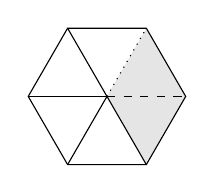
\begin{tikzpicture}
        \coordinate (O) at (0, 0);
        \coordinate (A) at ({cos(0)}, {sin(0)});
        \coordinate (B) at ({cos(60)}, {sin(60)});
        \coordinate (C) at ({cos(120)}, {sin(120)});
        \coordinate (D) at ({cos(180)}, {sin(180)});
        \coordinate (E) at ({cos(240)}, {sin(240)});
        \coordinate (F) at ({cos(300)}, {sin(300)});
        \fill[gray!20] (A) -- (B) -- (O) -- (F) -- cycle;
        \draw (A) -- (B) -- (C) -- (D) -- (E) -- (F) -- cycle;
        \draw[dashed] (O) -- (A); \draw[dotted] (O) -- (B); \draw (O) -- (C); \draw (O) -- (D); \draw (O) -- (E); \draw (O) -- (F);
    \end{tikzpicture}\\ (1) \end{tabular}
    \begin{tabular}{c}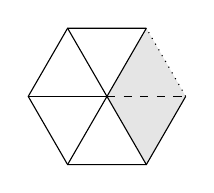
\begin{tikzpicture}
        \coordinate (O) at (0, 0);
        \coordinate (A) at ({cos(0)}, {sin(0)});
        \coordinate (B) at ({cos(60)}, {sin(60)});
        \coordinate (C) at ({cos(120)}, {sin(120)});
        \coordinate (D) at ({cos(180)}, {sin(180)});
        \coordinate (E) at ({cos(240)}, {sin(240)});
        \coordinate (F) at ({cos(300)}, {sin(300)});
        \fill[gray!20] (A) -- (B) -- (O) -- (F) -- cycle;
        \draw[dotted] (A) -- (B); \draw (B) -- (C) -- (D) -- (E) -- (F) -- (A);
        \draw[dashed] (O) -- (A); \draw (O) -- (B); \draw (O) -- (C); \draw (O) -- (D); \draw (O) -- (E); \draw (O) -- (F);
    \end{tikzpicture}\\ (2) \end{tabular}
    \begin{tabular}{c}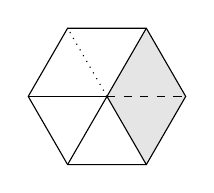
\begin{tikzpicture}
        \coordinate (O) at (0, 0);
        \coordinate (A) at ({cos(0)}, {sin(0)});
        \coordinate (B) at ({cos(60)}, {sin(60)});
        \coordinate (C) at ({cos(120)}, {sin(120)});
        \coordinate (D) at ({cos(180)}, {sin(180)});
        \coordinate (E) at ({cos(240)}, {sin(240)});
        \coordinate (F) at ({cos(300)}, {sin(300)});
        \fill[gray!20] (A) -- (B) -- (O) -- (F) -- cycle;
        \draw (A) -- (B) -- (C) -- (D) -- (E) -- (F) -- cycle;
        \draw[dashed] (O) -- (A); \draw (O) -- (B); \draw[dotted] (O) -- (C); \draw (O) -- (D); \draw (O) -- (E); \draw (O) -- (F);
    \end{tikzpicture}\\ (3) \end{tabular}
    \begin{tabular}{c}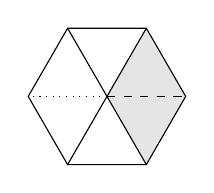
\begin{tikzpicture}
        \coordinate (O) at (0, 0);
        \coordinate (A) at ({cos(0)}, {sin(0)});
        \coordinate (B) at ({cos(60)}, {sin(60)});
        \coordinate (C) at ({cos(120)}, {sin(120)});
        \coordinate (D) at ({cos(180)}, {sin(180)});
        \coordinate (E) at ({cos(240)}, {sin(240)});
        \coordinate (F) at ({cos(300)}, {sin(300)});
        \fill[gray!20] (A) -- (B) -- (O) -- (F) -- cycle;
        \draw (A) -- (B) -- (C) -- (D) -- (E) -- (F) -- cycle;
        \draw[dashed] (O) -- (A); \draw (O) -- (B); \draw (O) -- (C); \draw[dotted] (O) -- (D); \draw (O) -- (E); \draw (O) -- (F);
    \end{tikzpicture}\\ (4) \end{tabular}
    \caption{Examples and counterexamples for building a manifold-like $1$-patching of a $2$-dimensional manifold-like triangulation. 
    (1) We have already added the edge patch along the dashed line and we add the edge patch along the dotted line.
    (2) The new edge patch may already be a subset of the subtriangulation
    (3) An inadmissible choice because the new edge patch has no overlap with current subtriangulation, though the next subtriangulation would be manifold-like
    (4) An inadmissible choice because the new edge patch has no overlap with current subtriangulation and the next subtriangulation would not be manifold-like.}\label{figure:illustrationpatching}
\end{figure}

% \begin{figure}
%     \centering
%     \begin{tabular}{c}\begin{tikzpicture}[scale=0.5]
%         \coordinate (O) at (0, 0);
%         \coordinate (A) at ({0.8*cos(  0)}, {0.8*sin(  0)});
%         \coordinate (B) at ({0.8*cos(120)}, {0.8*sin(120)});
%         \coordinate (C) at ({0.8*cos(240)}, {0.8*sin(240)});
%         \coordinate (X) at ({3.0*cos( 60)}, {3.0*sin( 60)});
%         \coordinate (Y) at ({3.0*cos(180)}, {3.0*sin(180)});
%         \coordinate (Z) at ({3.0*cos(300)}, {3.0*sin(300)});
%         \draw (A) -- (B) -- (C) -- cycle; \draw (X) -- (Y) -- (Z) -- cycle;
%         \draw[fill=gray!20] (X) -- (Y) -- (B) -- cycle;
%         \draw[fill=gray!20] (Y) -- (Z) -- (C) -- cycle;
%         \draw[fill=gray!20] (Z) -- (X) -- (A) -- cycle;
%         \draw[fill=gray!20] (A) -- (X) -- (B) -- cycle;
%         \draw[fill=gray!20] (B) -- (Y) -- (C) -- cycle;
%         \draw[fill=gray!20] (C) -- (Z) -- (A) -- cycle;
%     \end{tikzpicture}\\ (1) \end{tabular}
%     \begin{tabular}{c}\begin{tikzpicture}[scale=0.5]
%         \coordinate (O) at (0, 0);
%         \coordinate (A) at ({3.0*cos(  0)}, {3.0*sin(  0)});
%         \coordinate (B) at ({3.0*cos(120)}, {3.0*sin(120)});
%         \coordinate (C) at ({3.0*cos(240)}, {3.0*sin(240)});
%         \coordinate (X) at ({3.0*cos( 60)}, {3.0*sin( 60)});
%         \coordinate (Y) at ({3.0*cos(180)}, {3.0*sin(180)});
%         \coordinate (Z) at ({3.0*cos(300)}, {3.0*sin(300)});
%         \draw (O) -- (A);
%         \draw (O) -- (B);
%         \draw (O) -- (C);
%         \draw (O) -- (X);
%         \draw (O) -- (Y);
%         \draw (O) -- (Z);
%         %
%     \end{tikzpicture}\\ (2) \end{tabular}
%     \begin{tabular}{c}\begin{tikzpicture}[scale=0.5]
%         \tikzset{z={(90:1cm)}, y={(-30:1cm)}, x={(210:1cm)}}
%         % \tikzset{z={(90:1cm)}, y={(-10:1cm)}, x={(250:1cm)}}
% 
%         \coordinate (O) at (0, 0);
%         \coordinate (A) at ({3.0*cos(  0)}, {3.0*sin(  0)});
%         \coordinate (B) at ({3.0*cos(120)}, {3.0*sin(120)});
%         \coordinate (C) at ({3.0*cos(240)}, {3.0*sin(240)});
%         \coordinate (X) at ({3.0*cos( 60)}, {3.0*sin( 60)});
%         \coordinate (Y) at ({3.0*cos(180)}, {3.0*sin(180)});
%         \coordinate (Z) at ({3.0*cos(300)}, {3.0*sin(300)});
%         \coordinate (T) at ({0}, {0}, {3});
% 
%         \draw[thick, fill=gray!30] (O) -- (C) -- (T) -- cycle;
%         \draw[thick, fill=gray!30] (O) -- (Y) -- (T) -- cycle;
%         \draw[thick, fill=gray!30] (O) -- (Z) -- (T) -- cycle;
%         \draw[thick, fill=gray!30] (O) -- (A) -- (T) -- cycle;
%         \draw[thick, fill=gray!30] (O) -- (B) -- (T) -- cycle;
%         \draw[thick, fill=gray!30] (O) -- (X) -- (T) -- cycle;
% 
%     \end{tikzpicture}\\ (3) \end{tabular}
%     \caption{Example of a connected $2$-dimensional manifold triangulation, which triangulates an annulus, that does neither admit a manifold-like $0$-patching nor manifold-like $1$-patching.}\label{figure:annuluscounterexample}
% \end{figure}







% 3. Shellability 
\subsection{Shellable simplicial complexes}\label{subsection:shellability}


The notions of shelling and shellable triangulation have been discussed widely in combinatorial topology and polytopal theory. 
Formally, a triangulation is shellable if its full-dimensional simplices can be enumerated such that each simplex intersects the union of the previously listed simplices in a codimension one triangulation of a manifold. 
This forces the intermediate triangulations to be particularly well-shaped. 
We build upon the notion of shelling as introduced in~\cite[Definition 8.1]{ziegler1995lectures},
where our definition of shelling is equivalent to the notion of the shellings of simplicial complexes, see also~\cite[Remark~8.3]{ziegler1995lectures}. 

\todo[inline]{MV: Shortened, narrowed, removed repetitions.}

\mwl{Roughly speaking, a triangulation is shellable if the triangulation can be built, starting from a single simplex,
by successively gluing simplices to intermediate triangulations such that a combinatorial-geometric condition is satisfied:
the gluing interface is a triangulated submanifold of the boundary. 
This forces the intermediate triangulations to be particularly well-shaped. 
We turn our attention to a different idea of how to incrementally construct a simplicial complex while maintaining well-behaved intermediate complexes. 
It is often very helpful if a simplicial complex can be created recursively, starting with a single simplex, 
as this enables the inductive method of proof.}


Suppose that $\calT$ is an $n$-dimensional simplicial complex and we have an enumeration of the $n$-simplices $T_{0}, T_{1}, T_{2}, \dots \in \subsimplex_{n}(\calT)$.
For any enumeration, we call 
\begin{align*}
    I_m 
    := 
    \big( 
        T_{0} \cup T_{1} \cup \dots \cup T_{m} 
    \big) 
    \cap 
    T_{m+1}
\end{align*}
be the $m$-th \textit{interface set}. 
% Note that this intersection is automatically a subcomplex of the boundary complex of the last simplex $T_{m}$.
We call the enumeration a \emph{shelling} if each interface \cye{set} $I_m$ is a \cye{triangulated} manifold of dimension $n-1$. 

\begin{remark}
    We interpret a shelling as the construction of a triangulation 
    by successively attaching simplices such that the intermediate triangulations are well-behaved. 
    Conversely, the reverse enumeration describes a successive decomposition of the triangulation, hence the name ``shelling''.
\end{remark}
\begin{remark}
    Whether a simplicial complex is shellable can be checked, in principle, simply by trying out all the possible enumerations.
    That we cannot do much better than this is captured in the result that testing for shellability is NP-complete~\cite{goaoc2019shellability}:
    this complexity result is even true if we merely consider simplicial complexes of dimension two embedded in some Euclidean space.
\end{remark}


The reason of our interest in shellable simplicial complexes is that they can be constructed by \cye{a} successive adhesion of simplices to intermediate complexes \cye{where these intermediate complexes are} simplicial \disk s \cye{\sout{or a simplicial spheres}}, as shows the following important consequence.\todo{MV: OK? ``Intermediate'' excludes the last one.} 

\begin{lemma}\label{lemma:shell_triang_man}
    Let $\calT$ be an $n$-dimensional simplicial complex 
    with a shelling $T_{0}, T_{1}, T_{2}, \dots, T_{M}$,
    such that each simplex of dimension $n-1$ is contained in at most two simplices. 
    % DONE: what is non-branching?
    Then
    $$
        X_{m} := T_{0} \cup T_{1} \cup \dots \cup T_{m}
    $$ 
    is a \cye{triangulated} manifold with boundary for all $0 \leq m \leq M$.
    % 
    In particular, $X_{m}$ is a topological $n$-ball when $m < M$, 
    and 
    $X_{M}$ is either a topological $n$-ball or topological $n$-sphere. 
\end{lemma}
\begin{proof}  
    We prove this claim by induction. 
    Certainly, if $\calT$ contains only one single $n$-simplex, then it is a shellable triangulation of a topological $n$-ball. 
    Suppose that $X_m := T_{0} \cup T_{1} \cup \dots \cup T_{m}$ is a topological $n$-ball and that $T_{m+1}$ is the next $n$-simplex in the shelling.
    By definition, $I_{\cye{m}} := X_{m} \cap T_{m+1}$ is a submanifold of $\partial T_{m+1}$,
    and it is triangulated by some faces of $T_{m+1}$ and their subsimplices. 
    
    Let $F$ be such a face. 
    By assumption, $F$ must be contained in exactly one $n$-simplex of $T_{0}, T_{1}, \dots, T_{m}$,
    and $F$ is in the boundary of $X_{m}$. We conclude that $I_{m}$ triangulates a submanifold of the boundary of $X_{m}$.
    
    On the one hand, 
    if $I_{\cye{m}}$ is the entire boundary of $T_{m+1}$, 
    then it must also be the boundary of the topological $n$-ball $X_{m}$. 
    Hence $X_{m} \cup T_{m+1}$ must be a topological $n$-sphere and thus a manifold without boundary, which requires $m = M$.
    On the other hand, 
    if $I_{\cye{m}}$ is a proper subset of the entire boundary of $T_{m+1}$, 
    then $X_{m} \cup T_{m+1}$ is still a topological $n$-ball.
\end{proof}


We \cye{now} collect important examples of shellable triangulations. \cye{Essentially, in two space dimensions, interesting triangulations shellable, but starting from three space dimensions, nonshellable situations can arise}. Our main interest are local \cye{patches} (stars) within triangulations\cye{: these are shellable up to three space dimensions, but not necessarily beyond}. 

\begin{example}\label{example:shell_simpl}
    Any simplex $T$ \cye{(}trivially\cye{)} has a shelling. The boundary complex $\partial \calT(T)$ has a shelling:
    in fact, any enumeration of the boundary faces of $T$ constitutes a shelling\cye{, cf.~\cite[Example 8.2.(iii)]{ziegler1995lectures}}.
\end{example}
\begin{example}
    The standard triangulation of the $3$-dimensional cube by six tetrahedra, the Kuhn triangulation~\cite{kuhn1960some}, is shellable, as are its higher-dimensional generalizations.\footnote{We remark that Kuhn attributes this triangulation to Lefschetz~\cite{lefschetz2015introduction}.}
\end{example}

\cye{\begin{example}
    There exists a non-shellable triangulation of a tetrahedron and of a cube in $n=3$, see~\cite[Example 8.9]{ziegler1995lectures}.
\end{example}}\todo{MV: 3D counterexamples directly here and straight to the point.}


\begin{lemma}\label{lemma:shell_2D}
    Any simplicial $2$-\disk\ is shellable.
    Any simplicial $2$-sphere is shellable. 
\end{lemma}
\begin{proof}
    First, 
    let $\calS$ be any triangulation of a $2$-sphere. 
    By removing any triangle $S \in \calS$, we obtain a triangulation $\calT$ of a $2$-\disk.
    Any shelling of that \disk\ can be extended to a shelling of $\calS$ by re-inserting the first triangle $S$.
    So it remains to show that any triangulation $\calT$ of the two-dimensional \disk\ is shellable. 
    We will construct the shelling in reverse. 
    
    Write $M = |\calT|$. 
    There is nothing to show if $\calT$ contains only one triangle. 
    We call a triangle $T \in \calT$ \emph{good in $\calT$} if it intersects the boundary $\partial M$ in a non-empty union of edges. 
    Hence a triangle is good in $\calT$ if its intersection with $\partial M$ is either one, two, or three edges,
    and a triangle is not good in $\calT$ if that intersection is either empty, only some of its vertices, or a vertex and the opposite edge.
    % DONE: I understand what it means from the rest of the proof, but I believe it could a bit more explicit.
    We show by an induction argument over the number of triangles that every triangulation of a $2$-\disk\ that contains at least two triangles also contains at least two good triangles. 

    Clearly, this is the case if the triangulation of the $2$-\disk\ contains two triangles. 
    Now suppose the induction claim is true when the triangulation includes at most $N$ triangles,
    and assume that $\calT$ includes $N+1$ triangles. 
    There are at least two triangles with an edge on the boundary. 
    Suppose that $\calT$ does not have at least two triangles that are good in $\calT$.
    Then there exists a triangle $T'$ that intersects $\partial M$ 
    in one edge and its opposite vertex.
    Removing $T'$ splits the manifold into two \cye{face-}connected components, each of which is a topological $2$-\disk.
    By the induction assumption, each of those components contains at least two triangles 
    that are good in the respective component. 
    So each component has at least one triangle that is good in $\calT$. 
    Hence $\calT$ contains two good triangles, which completes the induction step. 
    
    We conclude that whenever $\calT$ triangulates a $2$-\disk,
    it contains a good triangle $T$. 
    If $T$ has three edges in the boundary, then $T = M$ and we are trivially done. 
    If $T$ intersects with the boundary in exactly one or two edges, 
    then $\overline{M \setminus T}$ is still a topological $2$-\disk.
    The triangulation $\calT'$ that is obtained by removing $T$
    is a triangulation of some $2$-\disk\ that intersects $T$ only at either two or one edges.
    Any shelling of $\calT'$ can \cye{in this way} be extended to a shelling of $\calT$\cye{, and} the proof is complete. 
\end{proof}

\begin{lemma}\label{lemma:stars_are_shellable}
    Let $\calT$ be a $n$-dimensional shellable triangulation and $V \in \Vertices(\calT)$ be a vertex.
    Then $\patch_{\calT}(V)$ is shellable. 
\end{lemma}
\begin{proof}
    This is Lemma~8.7 in \cite{ziegler1995lectures}.
%     Without loss of generality, $V$ is the origin. 
%     Any ray starting at $V$ intersects at most one vertex of $\patch_{\calT}(V)$.
%     We can also assume that all boundary vertices of $\patch_{\calT}(V)$ to be unit vectors,
%     which does not affect shellability. 
%     The simplicial boundary complex of $\calT$ is the boundary complex of a convex polytope,
%     and is thus shellable~\cite[Theorem~8.12]{ziegler1995lectures}. 
\end{proof}


\begin{lemma}
    Let $\calT$ be a $3$-dimensional manifold triangulation and $S \in \calT$.
    Then $\patch_{\calT}(S)$ is shellable. 
\end{lemma}
\begin{proof}
    \cye{For $S$ a tetrahedron, this is Example~\ref{example:shell_simpl}.}
    The statement is \cye{also} clear if $S$ is an inner or boundary face of $\calT$\cye{, where we only need to enumerate respectively one or two tetrahedra}. 
    The statement is \cye{still} easily verified if $S$ is an inner or boundary edge of $\calT$\cye{: one chooses a starting tetrahedron (with a boundary face) and rotates around the edge in a fixed direction to create a suitable enumeration}.

    \cye{When $S$ is an inner vertex, then the \cye{faces} (triangles) of $\patch_{\calT}(S)$ that do not contain $V$ constitute a simplicial $2$-sphere. Similarly, when $S$ is a boundary vertex, then the \cye{faces} (triangles) of $\patch_{\calT}(S)$ that do not contain $V$ constitute a simplicial $2$-\disk. Both these $2$-dimensional complexes are shellable \cye{by Lemma~\ref{lemma:shell_2D}}, and any such shelling \cye{immediately yields} a shelling of $\patch_{\calT}(S)$ since there is a one-to-one correspondance between the tetrahedra in $\calT$ and the triangles.}\footnote{\cye{For $S$ an inner vertex, \cite[Lemma~B.1]{ern2020stable} also yields the claim.}}\todo{MV: but not Lemma~\ref{lemma:stars_are_shellable}, because this first needs the triangulation $\calT$ itself to be shellable, right?}
\end{proof}

\begin{remark}
    Not all triangu\cye{l}able sets admit a triangulation that is shellable. 
    Moreover, even if a set admits a shellable triangulation, not all of its triangulations \cye{are} be shellable. \cye{For example, if we extend the non-shellable triangulation of a tetrahedron from~\cite[Example 8.9]{ziegler1995lectures}} to a triangulation of a hypertetrahedron by suspending it from a new point $v_\star$, 
    then the resulting new triangulation is non-shellable and coincides with the patch around $v_\star$.
    This demonstrates that patches around boundary simplices are not necessarily shellable when the \cye{space} dimension \cye{$n$} is larger than three.
\end{remark}\todo{MV: Moved up a bit.}


A major structural feature of shellable simplicial complexes 
is that each time a\cye{n $n$-}simplex is added, star\cye{s} around \cye{lower-dimensional} simpl\cye{ices} gets completed. 

\begin{lemma}\label{lemma:existenceofstar}
    Suppose that an $n$-dimensional manifold triangulation $\calT$ has a shelling $T_{0}, T_{1}, T_{2}, \dots, T_{M}$.
    For $0 \leq m < M$, write 
    $$
        X_{m} := T_{0} \cup T_{1} \cup \dots \cup T_{m},
        \qquad 
        I_{m} := X_{m} \cap T_{m+1}.
    $$ 
    \cye{\sout{Whenever} Then} $I_{m}$ is \cye{a} union of $k$ different face\cye{\sout{t}}s of $T$,\todo{MV: this is a property, not an assumption, right?} \cye{$1 \leq k \leq n$,} \cye{and} the intersection of those face\cye{\sout{t}}s is an interior simplex $S_{\cye{m}} \in \calT$ of dimension $n-k$ that satisfies 
    $$
        \patch_{X_{m+1}}(S_{\cye{m}}) = \patch_{\calT}(S_{\cye{m}}).
    $$
\end{lemma}
\begin{proof}
    We know $I_{m}$ is a \cye{triangulated} submanifold of the boundary of $T$, and so it must be a collection of $k$ face\cye{\sout{t}}s \cye{of $T$, $1 \leq k \leq n$ ($k = n + 1$ can happen for the last enumerated simplex $m = M$ when $\calT$ is an $n$-sphere). $I_{m}$ also} constitutes \cye{a} local patch \cye{(star) of $(n-1)$-dimensional simplices around} some simplex $S_{\cye{m}}$ of dimension $n-k$ \cye{in $I_{m}$}.
    By \cye{definition}, $S_{\cye{m}}$ \cye{is} be a boundary simplex of $X_{m}$\cye{,} and it is an interior simplex of $X_{m+1}$. 
    But then $S_{\cye{m}}$ cannot be a subsimplex of any of the simplices $T_{m+1}, \dots, T_{M}$,
    which means that $\patch_{X_{m+1}}(S_{\cye{m}}) = \patch_{\calT}(S_{\cye{m}})$. 
\end{proof}




\begin{remark}
    Not all trianguable sets admit a triangulation that is also shellable. 
    Moreover, even if a set admits a shellable triangulation, not all of its triangulations might be shellable. 
    We refer to~\cite[Example 8.9]{ziegler2012lectures} for an examples of non-shellable triangulations of cubes and tetrahedra in three dimensions. 

    For example, there exists a non-shellable triangulation of a tetrahedron. 
    If we extend this triangulation to a triangulation of a hypertetrahedron by suspending it from a new point $v_\star$, 
    then the resulting new triangulation is non-shellable and coincides with the patch around $v_\star$.
    This demonstrates that patches around boundary simplices are not necessarily shellable when the dimension is larger than the three.
\end{remark}


 








\section{Review of vector calculus and exterior calculus}\label{section:calculus}

% We discuss the Sobolev spaces of vector calculus and exterior calculus 
% with particular emphasis on their transformation behavior. 
% We refer the reader to Ern and Guermond~\cite{ern2021finite} and Hiptmair~\cite{hiptmair2002finite} for further background material on Sobolev vector analysis. 
% Exterior algebra and exterior products are reviewed in the textbooks by Greub~\cite{greub1967multilinear} and Lee~\cite{lee2012smooth}.
% TODO: Fuse these two paragraphs 

We review in this section the Sobolev spaces of vector and exterior calculus and their transformation behavior. We refer the reader to Ern and Guermond~\cite{ern2021finite} and Hiptmair~\cite{hiptmair2002finite} for background material on Sobolev vector analysis and to Greub~\cite{greub1967multilinear} and Lee~\cite{lee2012smooth} for exterior algebra and exterior products. 

Throughout this section, we let $\Omega \subseteq \bbR^{3}$ be any bounded open set.

\subsection{Vector calculus}

\cye{Recall the notations~\eqref{equation:W1p} and~\eqref{equation:W_curl_div_p} from Section~\ref{section:intro}; actually, here we temporarily rather employ }
\begin{gather*}
    W^{p}(\grad,\Omega) \cye{= W^{1,p}(\Omega)} = \{ u \in L^{p}(\Omega) \suchthat \grad v \in \bfL^{p}(\Omega) \}
    .
\end{gather*}
\mwl{Let $\Omega \subseteq \bbR^{3}$ be a bounded open set. 
First, recall that $L^{p}(\Omega)$ is the space of scalar-valued $p$-integrable functions defined on $\Omega$
and that $\bfL^{p}(\Omega) := L^{p}(\Omega)^{n}$ for vector-valued functions with each component in $L^{p}(\Omega)$. 
In the three-dimensional setting, we are particularly interested in the Sobolev vector analysis. 
% $W^{p}(\grad,\Omega) := W^{1,p}(\Omega)$ is 
The space of scalar-valued $L^{p}(\Omega)$ functions with weak gradients in $\bfL^{p}(\Omega)$ is 
\begin{gather*}
    W^{p}(\grad,\Omega) := W^{1,p}(\Omega) = \{ u \in L^{p}(\Omega) \suchthat \grad v \in \bfL^{p}(\Omega) \}
    .
\end{gather*}
The space $\bfW^{p}(\curl,\Omega)$ of vector-valued $\bfL^{p}(\Omega)$ functions with weak curls in $\bfL^{p}(\Omega)$
and the space of vector-valued $\bfL^{p}(\Omega)$ functions with weak divergences in $L^{p}(\Omega)$ are written 
\begin{gather*}
    \bfW^{p}(\curl,\Omega) = \{ \bfu \in \bfL^{p}(\Omega) \suchthat \curl \bfu \in \bfL^{p}(\Omega) \},
    \\ 
    \bfW^{p}(\divergence,\Omega) = \{ \bfu \in \bfL^{p}(\Omega) \suchthat \divergence \bfu \in L^{p}(\Omega) \}.
\end{gather*}}

We are interested in transformations of these Sobolev tensor fields from one domain onto another. 
Suppose that $\Omega, \Omega' \subset \mathbb{R}^3$ are open sets and suppose that $\phi: \Omega \to \Omega'$ is a bi-Lipschitz mapping.
\mwl{We introduce the} gradient-, curl-, and divergence-conforming Piola transformations, respectively, as the mappings 
$\phi^{\grad}: L^{p}(\Omega') \to L^{p}(\Omega)$,
$\phi^{\curl}: \bfL^{p}(\Omega') \to \bfL^{p}(\Omega)$, and 
$\phi^{\divergence}: \bfL^{p}(\Omega') \to \bfL^{p}(\Omega)$.
We also introduce 
$\phi^{\rm b}: L^{p}(\Omega') \to L^{p}(\Omega)$. 
We define them 
for any $v \in L^{p}(\Omega')$ and $\bfw \in \bfL^{p}(\Omega')$ by setting 
\begin{subequations}\label{eq_definition_piola}
\begin{align*}
    \phi^{\grad}(v) &= v \circ \phi, \\
    \phi^{\curl}(\bfw) &= \Jacobian\phi^{T} (\bfw \circ \phi), \\
    \phi^{\divergence}(\bfw) &= \adj(\Jacobian\phi) \left( \bfw \circ \phi \right), \\  
    \phi^{\rm b}(v) &= \det(\Jacobian\phi) \left( v \circ \phi \right),
\end{align*}
\end{subequations}
Here, $\Jacobian\phi$ is the Jacobian matrix of $\phi$ (see also~\cite[Definition~9.8]{ern2021finite}), and $\adj\Jacobian\phi$ denotes taking its adjugate matrix.
These transformations are invertible. 
Bounds on the Lebesgue norms will follow from a more general result below. 
We use the commutativity relations 
\begin{subequations}\label{eq_piola_commute}
\begin{align}
    \grad \phi^{\grad} (v) &= \phi^{\curl}(\grad v), 
    \\
    \curl \phi^{\curl}(\bfv) &= \phi^{\divergence}(\curl \bfv), 
    \\
    \divergence \phi^{\divergence}(\bfw) &= \phi^{\rm b}(\divergence \bfw),
\end{align}
\end{subequations}
where $v \in W^{p}(\grad,\Omega)$, $\bfv \in \bfW^{p}(\curl,\Omega)$, and $\bfw \in \bfW^{p}(\divergence,\Omega)$.  
We summarize this as a commuting diagram:
\begin{align*}
    \begin{CD}
        W^{p}(\grad,\Omega') @>{\grad}>> \bfW^{p}(\curl,\Omega') @>{\curl}>> \bfW^{p}(\divergence,\Omega') @>{\divergence}>> L^{p}(\Omega')
        \\
        @VV{\phi^{\grad}}V 
        @VV{\phi^{\curl}}V 
        @VV{\phi^{\divergence}}V 
        @VV{\phi^{\rm b}}V 
        \\
        W^{p}(\grad,\Omega ) @>{\grad}>> \bfW^{p}(\curl,\Omega ) @>{\curl}>> \bfW^{p}(\divergence,\Omega ) @>{\divergence}>> L^{p}(\Omega ).
    \end{CD}
\end{align*}

\begin{remark}
    The Piola transform goes into the opposite direction of the mapping $\phi : \Omega \rightarrow \Omega'$:
    % Our notion of Piola transform along a mapping $\phi : \Omega \rightarrow \Omega'$ goes in the opposite direction of the mapping:
    scalar and vector fields over $\Omega'$ are transformed into scalar and vector fields over $\Omega$.
    This definition is in accordance with the notion of pullback, which we will review shortly. 
    One advantage of that definition is that it also makes sense whenever the transformation is not onto. 
    The literature also knows the Piola transform in the direction of the original mapping. 
\end{remark}


\subsection{Exterior calculus}

%\cye{We now move to} exterior calculus. 
%We give a brief introduction into this topic, and refer to the literature for further background~\cite{lee2012smooth}. 

\mwl{We now move the discussion to exterior calculus, beginning with exterior algebra.}
Let $V$ be a real vector space. 
Given an integer $k \geq 0$, we let $\Alt^{k}(V)$ denote the space of scalar-valued antisymmetric $k$-linear forms over $V$. 
Recall that any $k$-linear scalar-valued form $u$ over $V$ is called antisymmetric
if 
\begin{gather*} 
    u( v_{\pi(1)}, v_{\pi(2)}, \ldots, v_{\pi(k)} ) 
    = 
    \text{sign}(\pi) 
    u( v_1, v_2, \ldots, v_k ) 
\end{gather*}
for any $v_1, v_2, \dots, v_k \in V$ and any permutation $\pi$ of the indices \(\{1, 2, \ldots, k\}\). 
By definition, $\Alt^{1}(V)$ is just the dual space of $V$, and $\Alt^{0}(V)$ is the space of real numbers. 
Formally, we define $\Alt^{k}(V)$ to be the zero vector space when $k < 0$. 

The wedge product (or exterior product) of alternating multilinear forms is a fundamental operation in exterior algebra. 
Given two alternating multilinear forms \( u_1 \in \Alt^{k}(V) \) and \( u_2 \in \Alt^{l}(V) \), 
their wedge product \( u_1 \wedge u_2 \) is a member of $\Alt^{k+l}(V)$
defined by the formula 
\begin{gather*}
    (u_1 \wedge u_2)(v_1, v_2, \ldots, v_{k+l}) 
    = 
    \frac{1}{k! l!} 
    % \sum_{ \pi \in S_{k+l}} 
    \sum_{ \pi } 
    \signum(\pi) 
    u_1( v_{\pi(  1)}, \ldots, v_{\pi(k  )} ) 
    u_2( v_{\pi(k+1)}, \ldots, v_{\pi(k+l)} ),
\end{gather*}
for any \( v_1, v_2, \ldots, v_{k+l} \in V \).
Here, the sum runs over all permutations $\pi$ of the index set \(\{ 1, 2, \ldots, k+l \}\).
% Here, \( S_{k+l} \) denotes the symmetric group on \( k+l \) elements, and \( \signum(\pi) \) is the sign of the permutation \( \pi \). 
The exterior product is bilinear and associative, and satisfies 
\begin{align*}
    u_1 \wedge u_2 = (-1)^{kl} u_2 \wedge u_1,
    \quad 
    \forall u_1 \in \Alt^{k}(V),
    \quad 
    \forall u_2 \in \Alt^{l}(V).
\end{align*}
We use the interior product, which is in some sense dual to the exterior product, in a special case. Given $v \in V$ and $u \in \Alt^{k}(V)$, we define $v \lrcorner u \in \Alt^{k-1}(V)$ via 
\begin{align*}
    (v \lrcorner u)( v_1, v_2, \ldots, v_{k-1} ) = u( v, v_1, v_2, \ldots, v_{k-1} ),
    \quad 
    \forall v_1, v_2, \ldots, v_{k-1} \in V.
\end{align*}

We are interested only in the special case $V = \bbR^{n}$ of alternating forms over the $n$-dimensional Euclidean space. 
Here, it is customary to identify $\Alt^{k}(V)$ with the space of antisymmetric tensors in $k$ indices. 
Moreover, this particular setting comes with a canonical basis. 
We let \(\{\cartanx^1, \cartanx^2, \ldots, \cartanx^{n}\}\) be the basis dual to the canonical unit vectors.
This is a canonical basis of $\Alt^{1}(\bbR^{n})$. 
To define a canonical basis of $\Alt^{k}(\bbR^{n})$, 
we first introduce $\Sigma(k,n)$, the set of strictly ascending mappings $\sigma : \{1,\dots,k\} \rightarrow \{1,\dots,n\}$,
and introduce the basic $k$-alternators 
\begin{align*}
    \cartanx^{\sigma} := \cartanx^{\sigma(1)} \wedge \dots \wedge \cartanx^{\sigma(k)}, 
    \quad 
    \forall \sigma \in \Sigma(k,n). 
\end{align*}
These define a basis of $\Alt^{k}(\bbR^{n})$.
Note that 
$\dim \Alt^{k}(\bbR^{n}) = \binom{n}{k}$. 
In particular, $\Alt^{k}(\bbR^{n})$ is the zero vector space whenever $k > n$.
% The dimension of the space of \(k\)-forms, denoted \(\bigwedge^{k} V\), is given by the binomial coefficient \(\binom{n}{k}\).

We notice that the canonical scalar product on $\bbR^{n}$ gives rise to a scalar product on $\Alt^{1}(\bbR^{n})$,
which induces a scalar product on $\Alt^{k}(\bbR^{n})$.
The basic $k$-alternators are an orthonormal basis of $\Alt^{k}(\bbR^{n})$ with respect to that inner product. 

\subsection{Smooth differential forms}

We write $C^{\infty}\Alt^{k}(\Omega)$ for the space of smooth differential $k$-forms over $\Omega \subseteq \bbR^{n}$,
which is the vector space of smooth mappings from $\Omega$ into $\Alt^{k}(\bbR^{n})$.
The exterior derivative \( \cartan \) is an operator that takes a \( k \)-form \( \omega \in C^{\infty}\Alt^{k}(\Omega) \) 
to a \((k+1)\)-form \( \cartan\omega \in C^{\infty}\Alt^{k+1}(\Omega) \). 
Every \( k \)-form \( \omega \in C^{\infty}\Alt^{k}(\Omega) \) can be written 
\begin{gather*}
    \omega = 
    \sum_{ \sigma \in \Sigma(k,n) } 
    \omega_{\sigma} \, 
    \cartanx^{\sigma(1)} \wedge \cartanx^{\sigma(2)} \wedge \cdots \wedge \cartanx^{\sigma(k)},
\end{gather*}
where \( \omega_{\sigma} : \Omega \rightarrow \bbR \) are smooth functions.
The exterior derivative \( \cartan\omega \) is defined by
\begin{gather*}
    \cartan\omega = 
    \sum_{ \sigma \in \Sigma(k,n) } 
    \sum_{j=1}^{n} 
    \frac{\partial \omega_{\sigma}}{\partial x^j} 
    \, \cartanx^j \wedge 
    \cartanx^{\sigma(1)} \wedge \cartanx^{\sigma(2)} \wedge \cdots \wedge \cartanx^{\sigma(k)}.
\end{gather*}
The exterior derivative is linear and nilpotent, which means 
\( \cartan(\cartan\omega) = 0 \) for any \( \omega \in C^{\infty}\Alt^{k}(\Omega) \).
Moreover, it satisfies the Leibniz rule:
\begin{gather*} 
    \cartan(\omega \wedge \eta) 
    = 
    \cartan\omega \wedge \eta + (-1)^{k} \omega \wedge \cartan\eta, 
    \qquad \forall \omega \in C^{\infty}\Alt^{k}(\Omega), 
    \qquad \forall \eta \in C^{\infty}\Alt^{l}(\Omega).
\end{gather*}

\subsection{Sobolev spaces of differential forms}

Let us now turn our attention to Sobolev spaces of differential forms. 
Since the exterior product space $\Alt^{k}(\bbR^{n})$ carries a norm, induced from the Euclidean norm on $\bbR^{n}$, we can consider the pointwise norms of differential $k$-forms. 
We let $L^{p}\Alt^{k}(\Omega)$ be the space of differential $k$-forms over $\Omega$ with locally integrable coefficients 
such that its pointwise norm is $p$-integrable. 
The exterior derivative is defined in the sense of distributions and we introduce 
\begin{gather*}
    W^{p}\Alt^{k}(\Omega) 
    := 
    \{ u \in L^{p}\Alt^{k}(\Omega) \suchthat \cartan u \in L^{p}\Alt^{k+1}(\Omega) \}
    .
\end{gather*}
We observe that $u \in L^{p}\Alt^{k}(\Omega)$ has weak exterior derivative $f \in L^{p}\Alt^{k+1}(\Omega)$
if and only if for all $v \in C^{\infty}_{c}\Lambda^{n-k-1}(\Omega)$ we have the integration by parts formula
\begin{align*}
    \int_{\Omega} \cartan v \wedge u
    &=
    (-1)^{k(n-k)+1}
    \int_{\Omega} v \wedge f 
    .
\end{align*}
% \mwl{We let $W^{p}_{0}\Alt^{k}(\Omega)$ be the closed subspace of those $u \in W^{p}\Alt^{k}(\Omega)$
% for which the extension by zero $\tilde u : \bbR^{n} \rightarrow \Alt^{k}(\bbR^{n})$ is a member of $\tilde u \in W^{p}\Alt^{k}(\bbR^{n})$.
% The space $W^{p}_{0}\Alt^{k}(\Omega)$ formalizes the idea of differential forms with vanishing boundary trace along the boundary $\partial\Omega$.}
% \cye{\sout{We let $W^{p}_{0}\Alt^{k}(\Omega)$ be the closed subspace of those $u \in W^{p}\Alt^{k}(\Omega)$ 
% for which the extension by zero $\tilde u : \bbR^{n} \rightarrow \Alt^{k}(\bbR^{n})$ is a member of $\tilde u \in W^{p}\Alt^{k}(\bbR^{n})$. }}\todo{MV: repeated below.}
Lastly, we are also interested in differential forms whose trace vanishes along a part of the boundary. 
Suppose that $\Gamma \subseteq \partial\Omega$ is a relatively open subset of the boundary. 
We say that $u \in W^{p}\Alt^{k}(\Omega)$ has vanishing trace along $\Gamma$ if for all $x \in \Gamma$ there exists $r > 0$
such that for all $v \in C^{\infty}_{c}\Lambda^{n-k-1}(B_r(x))$ we have the integration by parts formula
\begin{align*}
    \int_{B_r(x)} \cartan v \wedge \tilde u
    &=
    (-1)^{k(n-k)+1}
    \int_{B_r(x)} v \wedge \widetilde{\cartan u}
    .
\end{align*}
If that condition is satisfied, we also write 
\begin{align*}
    \trace_{\Gamma} u = 0
    .
\end{align*}
Accordingly, we write $\trace_{\Gamma} u = \trace_{\Gamma} u'$ for $\trace_{\Gamma} (u-u') = 0$ whenever $u, u' \in W^{p}\Alt^{k}(\Omega)$.
Lastly, we introduce the closed subspaces 
\begin{gather*}
    W^{p}_{0}\Alt^{k}(\Omega) 
    := 
    \{ u \in W^{p}\Alt^{k}(\Omega) \suchthat \trace_{\partial \Omega} u = 0 \}
    .
\end{gather*}
% \cye{The space $W^{p}_{0}\Alt^{k}(\Omega)$ formalizes the idea of differential forms with vanishing boundary trace along the boundary $\partial\Omega$.}\todo{MV: Moved here.}
\mwl{This is a closed subspace. We know that $u \in W^{p}_{0}\Alt^{k}(\Omega)$ if and only if its extension by zero $\tilde u : \bbR^{n} \rightarrow \Alt^{k}(\bbR^{n})$ is a member of $\tilde u \in W^{p}\Alt^{k}(\bbR^{n})$. Moreover, $\cartan W^{p}_{0}\Alt^{k}(\Omega) \subseteq W^{p}_{0}\Alt^{k+1}(\Omega)$.}


\subsection{Transformations by bi-Lipschitz mappings}

We are interested in transformations of Sobolev tensor fields from one domain onto \cye{an}other. 
Suppose that $\Omega,\Omega' \subset \bbR^{n}$ are open sets and suppose that $\phi: \Omega \to \Omega'$ is a bi-Lipschitz mapping.
The pullback of $u \in W^{p}\Alt^{k}(\Omega')$ along $\phi$ is the differential form 
\begin{align} \label{equation:pullback}
    \phi^{\ast}u_{|x}( v_{1}, v_{2}, \ldots, v_{k} ) 
    := 
    u_{|\phi(x)}( \Jacobian\phi_{|x} \cdot v_1, \Jacobian\phi_{|x} \cdot v_2, \ldots, \Jacobian\phi_{|x} \cdot v_k ) 
\end{align}
for any $v_1, v_2, \dots, v_k \in \bbR^{n}$ and any $x \in \Omega$. One can show that $\phi^{\ast}u \in W^{p}\Alt^{k}(\Omega)$.
We cite an explicit transformation estimate~\cite{licht2019smoothed}.

\begin{proposition} \label{proposition:pullbackestimate}
 Let $\phi : \Omega \rightarrow \Omega'$ be a bi-Lipschitz mapping between open sets $\Omega, \Omega' \subseteq \bbR^{n}$.
 Let $p \in [1,\infty]$ and $u \in L^{p}\Lambda^{k}(\Omega)$. 
 Then 
 \begin{align}\label{math:pullbackestimate}
  \begin{split}
  \| \phi^{\ast} u \|_{L^{p}\Lambda^{k}(\Omega)}
  &\leq 
  \| \Jacobian \phi \|^{k}_{L^{\cye{\infty}}(\Omega)}
  \| \det\Jacobian \phi^{-1} \|^{\frac{1}{p}}_{L^{\cye{\infty}}(\Omega')}
  \| u \|_{L^{p}\Lambda^{k}(\Omega')}
  .
  \end{split}
 \end{align}
\end{proposition}
\notice{MWL:I have simplified the statement to what is needed later.}


\begin{remark}
    In three dimensions, 
    the calculus of differential forms can be translated into classical vector calculus. 
    This is expressed formally as the commuting diagram 
    \begin{gather*}
    \begin{CD}
        C^\infty\Alt^0(\Omega) @>{\cartan}>> C^\infty\Alt^1(\Omega) @>{\cartan}>> C^\infty\Alt^2(\Omega) @>{\cartan}>> C^\infty\Alt^3(\Omega) 
        \\
        @VV{\varpi^{0}}V 
        @VV{\varpi^{1}}V 
        @VV{\varpi^{2}}V 
        @VV{\varpi^{3}}V 
        \\
        C^\infty(\Omega) @>{\grad}>> C^\infty(\Omega)^{3} @>{\curl}>> C^\infty(\Omega)^{3} @>{\divergence}>> C^\infty(\Omega)
    \end{CD}
    \cye{\, ,}
    \end{gather*}
    where $\varpi^{0}$ and $\varpi^{3}$ are the identity mappings and where 
    \begin{align*}
     \varpi^{1}\left( u_1 \cartanx^{1} + u_2 \cartanx^{2} + u_3 \cartanx^{3} \right) 
     &= 
     \left( u_1, u_2, u_3 \right), 
     \\
     \varpi^{2}\left( u_{12} \cartanx^{1} \wedge \cartanx^{2} + u_{13} \cartanx^{1} \wedge \cartanx^{3} + u_{23} \cartanx^{2} \wedge \cartanx^{3} \right) 
     &= 
     \left( u_{23}, - u_{13}, u_{12} \right).   
    \end{align*}
    In two dimensions, 
    the calculus of differential forms can be translated into 2D vector calculus in two different ways. 
    To the authors' best knowledge, neither convention is dominant in the literature.
    We summarize the situation in the following commuting diagram: 
    \begin{gather*} 
    \begin{CD}
        C^\infty(\Omega) @>{\curl}>> C^\infty(\Omega)^{2} @>{\divergence}>> C^\infty(\Omega)
        \\
        @AA{\varkappa^{0}}A 
        @AA{\varkappa^{1}}A 
        @AA{\varkappa^{2}}A 
        \\
        C^\infty\Alt^0(\Omega) @>{\cartan}>> C^\infty\Alt^1(\Omega) @>{\cartan}>> C^\infty\Alt^2(\Omega) 
        \\
        @VV{\varpi^{0}}V 
        @VV{\varpi^{1}}V 
        @VV{\varpi^{2}}V 
        \\
        C^\infty(\Omega) @>{\grad}>> C^\infty(\Omega)^{2} @>{\rot}>> C^\infty(\Omega)
    \end{CD}
    \cye{\,.}
    \end{gather*}
    Here, $\varpi^{1}\left( u_1 \cartanx^{1} + u_2 \cartanx^{2} \right) = \left( u_1, u_2 \right)$ is the lower middle isomorphism. We introduce the rotation operator $J(x,y) = (y,-x)$ and define $\varkappa = J \varpi$ and $\rot = \divergence J$.
    The other vertical arrows are the identity. 
    The utility of exterior calculus is that the operators of vector calculus can be translated into a common framework that does not depend on the dimension.
\end{remark}

\subsection{Some approximation properties}

We finally review a few approximation properties. 
Let $\mollifier$ be a non-negative scalar function supported in the unit ball around the origin and with unit integral.
Define $\mollifier_{\eps}(x) := \eps^{-n} \mollifier(x/\eps)$. We review the following approximation results.

\begin{lemma}
%     Let $\Omega \subseteq \bbR^{n}$ be a bounded open set and let $u : \Omega \rightarrow \bbR$ be locally integrable.  
%     Then $\mollifier_{\epsilon} \star u \rightarrow u$ almost everywhere. 
%     If $u \in L^{p}(\Omega)$ for some $1 \leq p < \infty$, then $u_{\epsilon} \rightarrow u$ in $L^{p}(\Omega)$.
    Let $\Omega \subseteq \bbR^{n}$ be a bounded open set and let $1 \leq p < \infty$. 
    If $u \in L^{p}(\Omega)$, then the convolution $\mollifier_{\eps} \star u \rightarrow u$ in $L^{p}(\Omega)$ as $\epsilon \rightarrow 0$.
\end{lemma}

% \begin{lemma} % TODO: possibly useful
%     Let $1 \leq p < \infty$. A sequence converges to $u \in L^{p}$ if and only if it converges locally by measure and the $L^{p}$ norms converge.
% \end{lemma}

\begin{lemma}
    Let $\Omega \subseteq \bbR^{n}$ be a bounded open set and let $1 \leq p < \infty$. 
    Smooth forms are dense in $W^{p}\Lambda^{k}(\Omega)$.
    If $\Omega$ is convex, then $C^{\infty}_{c}\Lambda^{k}(\Omega)$ is dense in $W^{p}_{0}\Lambda^{k}(\Omega)$.
\end{lemma}
\begin{proof}
    We notice $\mollifier_{\epsilon} \star u \in C^{\infty}\Lambda^{k}(\bbR^{n})$. 
    By the dominated convergence theorem and because $u$ has a weak derivative,
    for any $v \in C^{\infty}_{c}\Lambda^{n-k-1}(\Omega)$
    \begin{align*}
        \int_{\bbR^{n}} ( \mollifier_{\epsilon} \star u ) \wedge \cartan v 
        &= 
        \int_{\bbR^{n}} \int_{\bbR^{n}} \mollifier(x-y) \wedge u(y) \wedge \cartan_{x} v(x) \;dx\,dy
        \\&= 
        \int_{\bbR^{n}} \int_{\bbR^{n}} \cartan_x\mollifier(x-y) \wedge u(y) \wedge v(x) \;dx\,dy
        \\&= 
        - \int_{\bbR^{n}} \int_{\bbR^{n}} \cartan_y\mollifier(x-y) \wedge u(y) \wedge v(x) \;dx\,dy
        \\&= 
        \int_{\bbR^{n}} \int_{\bbR^{n}} \mollifier(x-y) \wedge \cartan_y u(y) \wedge v(x) \;dx\,dy
        = 
        \int_{\bbR^{n}} ( \mollifier_{\epsilon} \star \cartan u ) \wedge v 
        .
    \end{align*}
    Hence $C^{\infty}\Lambda^{k}(\Omega)$ is dense in $W^{p}\Lambda^{k}(\Omega)$.
    
    Next, suppose that $\Omega$ is convex. Without loss of generality, $0 \in \Omega$. 
    Let $u \in W^{p}_{0}\Lambda^{k}(\Omega)$ and extend $u$ trivially onto $\bbR^{n}$. 
    Define $\varphi_t(x) = tx$ for $t > 1$. 
    Then $\varphi_{t}^{\ast} u \in W^{p}_{0}\Lambda^{k}(t^{-1}\Omega)$ 
    and $\varphi_{t}^{\ast} u$ converges to $u$ as $t$ decreases towards $1$. 
    Given any $t > 1$, by taking the convolution with $\mollifier_{\epsilon}$ for $\epsilon > 0$ small enough,
    we approximate $\varphi_{t}^{\ast} u$ through members of $C^{\infty}_{c}\Lambda^{k}(\Omega)$.
    The desired result follows. 
\end{proof}
















\section{Regularized potential operators over convex sets}\label{section:potentialoperator}


{\color{red}
We want to bound Poincar\'e--Friedrichs constants for the exterior derivative over convex domains.
We already know the optimal constants for the gradient operator over convex domains,
and we know bounds for the Poincar\'e--Friedrichs constants for the entire $L^{2}$ de~Rham complex. 
We are not aware of such bounds for the case of the $L^{p}$ de~Rham complex when $1 \leq p \leq \infty$. 

For that reason, we bound the norms of regularized potential operators for the exterior derivative over convex domains.
We solve this for two special cases: either the $L^{p}$ de~Rham complex without boundary conditions, 
and the $L^{p}$ de~Rham with full boundary conditions. 
The corresponding potential operators are known as the regularized Poincar\'e and regularized Bogovski\u{\i} potentials in the literature. 
We build upon the discussion spearheaded by Costabel and McIntosh~\cite{costabel2010bogovskiui},
who analyze them as pseudodifferential operators over domains star-shaped with respect to a ball. 
% 
In comparison to their work, our discussion is more modest:
we study potential operators merely over convex sets, and we are only interested in their operator norms between Lebesgue spaces.
However, our purpose are explicit bounds for the operator norms, which are of independent interest. 

In what follows, $\Omega \subseteq \bbR^{n}$ is a convex bounded open set with diameter $\diam(\Omega) > 0$.
}

We \cye{now give} bounds for Poincar\'e--Friedrichs constants for the exterior derivative over convex domains\cye{, in} two special cases\todo{MV: Discussion already in the introduction, or in Remark~\ref{remark:reg_Poinc_Bog}}: 
either the $L^{p}$ de~Rham complex without boundary conditions, \cye{or} the $L^{p}$ de~Rham with full boundary conditions. 
The corresponding potential operators are known as the regularized Poincar\'e and regularized Bogovski\u{\i} potentials in the literature. 
We build upon the discussion spearheaded by Costabel and McIntosh~\cite{costabel2010bogovskiui},
who analyze them as pseudo\cye{-}differential operators over domains star-shaped with respect to a ball. 
In comparison to their work, our discussion is more modest:
we study potential operators merely over convex sets, and we are only interested in their operator norms between Lebesgue spaces.
However, our purpose are explicit bounds for the operator norms, \cye{giving the Poincar\'e--Friedrichs constants}. Let $\Omega \subseteq \bbR^{n}$ is a convex bounded open\todo{MV: Weakly Lipschitz??} set with diameter $\cye{\diam(\Omega)} > 0$\todo{MV: Unifying the notation.}.





\subsection{Regularized Poincar\'e and Bogovski\u{\i} operators}

We begin with introducing the Costabel-McIntosh kernel.
For any $\ell \in \{0,\dotsc,n\}$, we define the kernel $G_{\ell} : \bbR^{n} \times \bbR^{n} \rightarrow \bbR$ by
\begin{equation}\label{math:mainkernel}
  G_{\ell}(x,y) = \int_{1}^\infty (t-1)^{n-\ell}t^{\ell-1} \vol(\Omega)^{-1}\chi_{\Omega} \left(y+t(x-y)\right)\,dt
  .
\end{equation}
Given a differential form $u \in {C^\infty_c}(\bbR^n,\Alt^\ell)$, where \(1 \leq \ell \leq n\), 
we then define the integral operators
\begin{align*}
  \Poinc_{\ell} u(x) &= \int_{\Omega} G_{n-\ell+1}(y,x) \,(x-y)\lrcorner u(y)\,dy,
  \\
  \Bogov_{\ell} u(x) &= \int_{\Omega} G_{\ell}(x,y) \,(x-y)\lrcorner u(y)\,dy.
\end{align*}
We call $\Poinc_{\ell}$ the Poincar\'e operator and $\Bogov_{\ell}$ the Bogovski\u{\i} operator. 

We show that the integrals in the definition of $\Poinc_{\ell}$ and $\Bogov_{\ell}$ actually exist. 
In order to analyze the properties of the potential operators,
we first rewrite the Costabel-McIntosh kernel $G_{\ell}$.
Letting $x,y \in \bbR^n$ with $x \neq y$, we find 
\begin{align*}
    G_{\ell}(x,y) 
    &= 
    \int_{0}^{\infty} t^{n-\ell} (t+1)^{\ell-1} \vol(\Omega)^{-1} \chi_{\Omega} \left( x+t(x-y) \right)\,dt
    \\
    &= 
    \int_{0}^{\infty} \sum_{k=0}^{\ell-1} \tbinom{\ell-1}{k} t^{n-\ell+k} \vol(\Omega)^{-1} \chi_{\Omega} \left( x+t(x-y) \right)\,dt
    \\
    &= 
    \int_{0}^{\infty} \sum_{k=0}^{\ell-1} \tbinom{\ell-1}{\ell-1-k} t^{n-\ell+\ell-1-k} \vol(\Omega)^{-1} \chi_{\Omega} \left( x+t(x-y) \right)\,dt
    \\
    &= 
    \int_{0}^{\infty} \sum_{k=0}^{\ell-1} \tbinom{\ell-1}{k} t^{n-k-1} \vol(\Omega)^{-1} \chi_{\Omega} \left( x+t(x-y) \right)\,dt
    \\
    &= 
    \sum_{k=0}^{\ell-1} \tbinom{\ell-1}{k} \int_{0}^{\infty} t^{n-k-1} \vol(\Omega)^{-1} \chi_{\Omega}\left( x+t(x-y) \right)\,dt 
    \\
    &= 
    \vol(\Omega)^{-1} \sum_{k=0}^{\ell-1} \tbinom{\ell-1}{k} \, |x-y|^{k-n} \int_{0}^{\infty} r^{n-k-1} \chi_{\Omega}\left(x+r\frac{x-y}{|x-y|}\right)\,dr
    .
\end{align*}
If $x, y \in \Omega$, then we can restrict the inner integrals to the range $0 \leq r \leq \diam(\Omega)$, which gives 
\begin{align*}
    G_{\ell}(x,y) 
    &= 
    \vol(\Omega)^{-1} \sum_{k=0}^{\ell-1}\tbinom{\ell-1}{k} |x-y|^{k-n} \int_{0}^{\diam(\Omega)} r^{n-k-1} \,dr 
    \\
    &= 
    \vol(\Omega)^{-1} \sum_{k=0}^{\ell-1}\tbinom{\ell-1}{k} |x-y|^{k-n} \frac{ \diam(\Omega)^{n-k} }{n-k}.
\end{align*}
We are now in a position to show that the potentials are bounded with respect to Lebesgue norms. 

\subsection{\cye{An operator norm bound with respect to the Lebesgue norm: the Poincar\'e case}}

We begin with the Poincar\'e operator. 
Let $B_{\diam(\Omega)}(0)$ be the $n$-dimensional ball centered at the origin.
Suppose that $u \in L^{\infty}\Alt^{\ell}(\Omega)$ with $1 \leq \ell \leq n$.
We pointwise estimate $\Poinc_{\ell} u(x)$ for any $x \in \Omega$ by the result of a convolution of a locally integrable function with $u$:
\begin{align*}
    \left| \Poinc_{\ell} u(x) \right|
    &=
    \left| 
        \int_{\Omega} G_{n-\ell+1}(x,y) \,(x-y)\lrcorner u(y)\,dy
    \right| 
%     \\&\leq 
%     \int_{\Omega} \vol(\Omega)^{-1} \sum_{k=0}^{(n-\ell+1)-1}\tbinom{(n-\ell+1)-1}{k} \frac{ \diam(\Omega)^{n-k} }{n-k} |x-y|^{k+1-n} |u(y)| \,dy
    \\&\leq 
    \int_{\Omega} \vol(\Omega)^{-1} \sum_{k=0}^{ n-\ell }\tbinom{ n-\ell }{k} \frac{ \diam(\Omega)^{n-k} }{n-k} |x-y|^{k+1-n} \chi_{B_{\diam(\Omega)}(0)}(x-y) |u(y)| \,dy
    .
\end{align*}
We recall the radial integrals 
\begin{align*}
    \int_{B_{\diam(\Omega)}(0)} |z|^{k+1-n} \,dz
    &
    =
    \vol_{n-1}(S_1) \int_{0}^{\diam(\Omega)} r^{k+1-n} r^{n-1} \,dr
    \\&
    =
    \vol_{n-1}(S_1) \int_{0}^{\diam(\Omega)} r^{k} \,dr
    =
    \vol_{n-1}(S_1) \frac{\diam(\Omega)^{k+1}}{k+1}
    ,
\end{align*}
where $S_1 \subseteq \bbR^{n}$ stands for the unit sphere of dimension $n-1$. 
We compute 
\begin{align}
    &
    \int_{\bbR^{n}} \sum_{k=0}^{n-\ell} \tbinom{n-\ell}{k} \frac{ \diam(\Omega)^{n-k} }{n-k} \chi_{B_{\diam(\Omega)}(0)}(z) |z|^{k+1-n} \,dz
    \\&
    =
    \sum_{k=0}^{n-\ell} \tbinom{n-\ell}{k} \frac{ \diam(\Omega)^{n-k} }{n-k} \int_{B_{\diam(\Omega)}(0)} |z|^{k+1-n} \,dz
    \\&
    =
    \vol_{n-1}(S_1) \sum_{k=0}^{n-\ell} \tbinom{n-\ell}{k} \frac{ \diam(\Omega)^{n-k} }{n-k} \frac{\diam(\Omega)^{k+1}}{k+1}
    %\\&
    =
    \vol_{n-1}(S_1) \diam(\Omega)^{n+1} \underbrace{ \sum_{k=0}^{n-\ell} \frac{ \tbinom{n-\ell}{k} }{ (n-k)(k+1) } }_{ =: A_{\Poinc}(n,\ell) \leq 2^{n-\ell}}
    \label{equation:A_Poinc}
    .
\end{align}
Here, $A_{\Poinc}(n,\ell)$ is a numerical constant that depends only on $n$ and $\ell$ 
and which is bounded by $2^{n-\ell}$. 
In particular, the integral $\Poinc_{\ell} u(x)$ is absolutely convergent for any choice of $x \in \Omega$. 
So the convolution of $u$ is taken against an integrable function. 
Young's convolution inequality now implies: 
\begin{align*}
    \| \Poinc_{\ell} u \|_{L^{p}(\Omega)}
    &
    \leq 
    \vol_{n-1}(S_1) A_{\Poinc}(n,\ell) \frac{ \diam(\Omega)^{n} }{\vol(\Omega)} 
    \diam(\Omega)
    \| u \|_{L^{p}(\Omega)}
    \\&
    \leq 
    n A_{\Poinc}(n,\ell) \frac{ \vol_{n}(B_{\diam(\Omega)}(0)) }{\vol(\Omega)} 
    \diam(\Omega)
    \| u \|_{L^{p}(\Omega)}
    .
\end{align*}
We have assumed so far that $u \in L^{\infty}\Alt^{\ell}(\Omega)$. 
Since that space is dense in the Lebesgue spaces, a density argument establishes the following: 
for any $1 \leq p \leq \infty$ we have a bounded linear operator 
\begin{gather*}
    \Poinc_{\ell} : L^{p}\Alt^{\ell}(\Omega) \rightarrow L^{p}\Alt^{\ell-1}(\bbR^n).
\end{gather*}
% Its operator norm is bounded by $n A_{\Poinc}(n,\ell) \vol(\Omega)^{-1} \vol_{n}(B_{\diam(\Omega)}(0)) \diam(\Omega)$. 
% 


\subsection{\cye{An operator norm bound with respect to the Lebesgue norm: the Bogovski\u{\i} case}}

We analyze the Bogovski\u{\i} potential operator by similar means. 
Suppose that $u \in L^{\infty}\Alt^{\ell}(\bbR^{n})$ with $\supp u \subseteq \overline\Omega$ and that $x \in \bbR^{n}$.
First, if $x \notin \Omega$, then the convexity of $\Omega$ implies that $y + t( x - y ) \notin \Omega$ for all $t > 1$. Hence $G(x,y) = 0$ and therefore $\Bogov_{\ell} u(x) = 0$ in that case.
Consider now the case $x \in \overline\Omega$. 
We estimate $\Bogov_{\ell} u(x)$ pointwise by 
\begin{align*}
    \left| \Bogov_{\ell} u(x) \right|
    &=
    \left| 
        \int_{\Omega} G_{\ell}(x,y) \,(x-y)\lrcorner u(y)\,dy
    \right| 
    \\&\leq 
    \int_{\Omega} \vol(\Omega)^{-1} \sum_{k=0}^{\ell-1}\tbinom{\ell-1}{k} \frac{ \diam(\Omega)^{n-k} }{n-k} |x-y|^{k+1-n} |u(y)| \,dy
    \\&\leq 
    \int_{\bbR^{n}} \vol(\Omega)^{-1} \sum_{k=0}^{\ell-1}\tbinom{\ell-1}{k} \frac{ \diam(\Omega)^{n-k} }{n-k} \chi_{B_{\diam(\Omega)}(0)}(x-y) |x-y|^{k+1-n} |u(y)| \,dy
    .
\end{align*}
Using once more the radial integrals discussed above, we compute 
% We recall the radial integrals 
% \begin{align*}
%     \int_{B_{\diam(\Omega)}(0)} |z|^{k+1-n} dz
%     =
%     \vol_{n-1}(S_1) \int_{0}^{\diam(\Omega)} r^{k+1-n} r^{n-1} dr
%     =
%     \vol_{n-1}(S_1) \int_{0}^{\diam(\Omega)} r^{k} dr
%     =
%     \vol_{n-1}(S_1) \frac{\diam(\Omega)^{k+1}}{k+1}
%     .
% \end{align*}
% We compute 
\begin{align*}
    &
    \int_{\bbR^{n}} \sum_{k=0}^{\ell-1} \tbinom{\ell-1}{k} \frac{ \diam(\Omega)^{n-k} }{n-k} \chi_{B_{\diam(\Omega)}(0)}(z) |z|^{k+1-n} \,dz
    \\&
    =
    \sum_{k=0}^{\ell-1} \tbinom{\ell-1}{k} \frac{ \diam(\Omega)^{n-k} }{n-k} \int_{B_{\diam(\Omega)}(0)} |z|^{k+1-n} \,dz
    \\&
    =
    \vol_{n-1}(S_1) \sum_{k=0}^{\ell-1} \tbinom{\ell-1}{k} \frac{ \diam(\Omega)^{n-k} }{n-k} \frac{\diam(\Omega)^{k+1}}{k+1}
    %\\&
    =
    \vol_{n-1}(S_1) \diam(\Omega)^{n+1} \underbrace{ \sum_{k=0}^{\ell-1} \frac{ \tbinom{\ell-1}{k} }{ (n-k)(k+1) } }_{ =: A_{\Bogov}(n,\ell) \leq 2^{\ell-1}}
    \label{equation:A_Bogov}
    .
\end{align*}
Here, $A_{\Bogov}(n,\ell)$ is a numerical constant that depends only on $n$ and $\ell$ 
and which is bounded by $2^{\ell-1}$. 
In particular, the integral $\Bogov_{\ell} u(x)$ is absolutely convergent for any choice of $x \in \bbR^{n}$. 
So the convolution of $u$ is taken against an integrable function. 
Young's convolution inequality now implies: 
\begin{align*}
    \| \Bogov_{\ell} u \|_{L^{p}(\Omega)}
    &
    \leq 
    \vol_{n-1}(S_1) A(n,\ell) \frac{ \diam(\Omega)^{n} }{\vol(\Omega)} 
    \diam(\Omega)
    \| u \|_{L^{p}(\Omega)}
    \\&
    \leq 
    n A_{\Bogov}(n,\ell) \frac{ \vol_{n}(B_{\diam(\Omega)}(0)) }{\vol(\Omega)} 
    \diam(\Omega)
    \| u \|_{L^{p}(\Omega)}
    .
\end{align*}
We have assumed so far that $u$ is essentially bounded.
Since that space is dense in the Lebesgue spaces, a density argument yields: 
for any $1 \leq p \leq \infty$ we have a bounded linear operator 
\begin{gather*}
    \Bogov_{\ell} : L^{p}\Alt^{\ell}(\Omega) \rightarrow L^{p}\Alt^{\ell-1}(\bbR^n).
\end{gather*}
% Its operator norm is bounded by $n A_{\Bogov}(n,\ell) \vol(\Omega)^{-1} \vol_{n}(B_{\diam(\Omega)}(0)) \diam(\Omega)$. 
Moreover, $\supp \Bogov_{\ell} u \subseteq \overline\Omega$,
that is, the reconstructed potential has support contained within $\overline\Omega$. 
\\





\subsection{Additional properties}

Additional properties of these operators become apparent after a change of variables. 
We write down the full definition of these operators and perform two substitutions.
For the Poincar\'e operator, we substitute $a = x + t(y-x)$ and then we substitute $s = (t-1)/t$,
leading to 
\begin{align*}
    \Poinc_{\ell} u(x) 
    &= 
    \int_{\Omega} \int_{1}^\infty (t-1)^{\ell-1}t^{n-\ell} 
    \chi_{\Omega}\left(x+t(y-x)\right) 
    (x-y)\lrcorner u(y) \,dt\,dy 
    \\
    &=
    \int_{\bbR^{n}} \chi_{\Omega}(a) \,(x-a)\lrcorner \int_{0}^{1} t^{\ell-1} u\left(a+t(x-a)\right)\,dt\,da
    .
\end{align*}
For the Bogoski\u{\i} operator, we substitute $a = y + t(x-y)$ and then we substitute $s = t/(t-1)$,
leading to 
\begin{align*}
    \Bogov_{\ell} u(x) 
    &= 
    \int_{\Omega} \int_{1}^\infty (t-1)^{n-\ell}t^{\ell-1} 
    \chi_{\Omega}\left(y+t(x-y)\right) 
    (x-y)\lrcorner u(y) \,dt\,dy 
    \\
    &=
    - \int_{\bbR^{n}} \chi_{\Omega}(a) \,(x-a)\lrcorner \int_{1}^\infty t^{\ell-1} u\left(a+t(x-a)\right)\,dt\,da
    .
\end{align*}
% We first discuss the support properties of this operator. 
% Suppose that $u \in C^{\infty}\Alt^{\ell-1}(\bbR^n)$ satisfies $\supp u \subseteq \overline\Omega$.
% Then $\Bogov_{\ell} u(x) = 0$ whenever $x \notin \overline\Omega$,
% meaning $\supp \Bogov_{\ell} u \subseteq \overline\Omega$.
% 
Given $a \in \Omega$, we introduce the potential operators 
\begin{align*}
    \Poinc_{\ell,a} u(x) 
    &:= 
    (x-a)\lrcorner \int_{0}^{1} t^{\ell-1} u\left(a+t(x-a)\right)\,dt
    ,
    \\
    \Bogov_{\ell,a} u(x) 
    &:= 
    - (x-a)\lrcorner \int_{1}^\infty t^{\ell-1} u\left(a+t(x-a)\right)\,dt
    .
\end{align*}
By definition,
\begin{align*}
    \Poinc_{\ell} u(x) 
    =
    \int_{\Omega} \Poinc_{\ell,a} u(x) \,da,
    \quad 
    \Bogov_{\ell} u(x) 
    =
    \int_{\Omega} \Bogov_{\ell,a} u(x) \,da
    .
\end{align*}
We study the interaction of these potential operator with the exterior derivative in more detail.
% 
That discussion is classical and establishes the exactness of several de~Rham complexes. 
We recapitulate these arguments since our variants of the regularized potential operators 
are not yet included in the published literature. 

Suppose that $u \in C^{\infty}\Alt^{\ell}(\bbR^n)$.
We rewrite the Poincar\'e potential,
\begin{align*}
    \Poinc_{\ell,a} u(x) 
    &= 
    (x-a)\lrcorner \int_{0}^{1} t^{\ell-1} u\left(a+t(x-a)\right)\,dt\,da\;
    \\&
    = 
    (x-a)\lrcorner 
    \sum_{\sigma \in \Sigma(k,n)}
    \int_{0}^{1} 
    t^{\ell-1} u_{\sigma}\left(a+t(x-a)\right) \cartanx^{\sigma} \,dt 
    \\&
    = 
    \sum_{\sigma \in \Sigma(k,n)} \sum_{i=1}^{k}
    \int_{0}^{1} 
    t^{\ell-1} u_{\sigma}\left(a+t(x-a)\right) (-1)^{i-1} (x-a)_{\sigma(i) } \,\cartanx^{\sigma-\sigma(i)} \,dt 
    ,
\end{align*}
and compute its exterior derivative:
\begin{align*}
    \cartan \Poinc_{\ell,a} u(x) 
    &= 
    \ell
    \sum_{\sigma \in \Sigma(k,n)} \sum_{i=1}^{k}
    \int_{0}^{1} 
    t^{\ell-1} u_{\sigma}\left(a+t(x-a)\right) \,\cartanx^{\sigma-\sigma(i)} \,dt 
    \\&\qquad
    + 
    \sum_{\sigma \in \Sigma(k,n)} \sum_{i=1}^{k} \sum_{j=1}^{n}
    \int_{0}^{1} 
    t^{\ell} \frac{ \partial u_{\sigma} }{\partial x_{j}}\left(a+t(x-a)\right) (-1)^{i-1} (x-a)_{\sigma(i) } \,\cartanx^{j} \wedge \cartanx^{\sigma-\sigma(i)} \,dt 
    .
\end{align*}
We write the exterior derivative of $u$ as 
\begin{align*}
    \cartan u(x)
    =
    \sum_{\sigma \in \Sigma(k,n)} \sum_{j=1}^{n}
    \frac{ \partial u }{\partial x_{j}}(x) \,\cartanx^{j} \wedge \cartanx^{\sigma} \,dt 
    ,
\end{align*}
and apply the Poincar\'e potential operator to this result, which gives 
\begin{align*}
    \Poinc_{\ell+1,a} \cartan u(x)
    &=
    (x-a)\lrcorner 
    \sum_{\sigma \in \Sigma(k,n)} \sum_{j=1}^{n}
    \int_{0}^{1} t^{\ell} \frac{ \partial u_{\sigma} }{\partial x_{j}}\left(a+t(x-a)\right) \,dt 
    \,\cartanx^{j} \wedge \cartanx^{\sigma}
    \\&
    = 
    \sum_{\sigma \in \Sigma(k,n)} \sum_{j=1}^{n}
    \int_{0}^{1} t^{\ell} \frac{ \partial u_{\sigma} }{\partial x_{j}}\left(a+t(x-a)\right) \,dt (x-a)_{j}
    \,\cartanx^{\sigma}
    \\&\qquad 
    - 
    \sum_{\sigma \in \Sigma(k,n)} \sum_{i=1}^{k} \sum_{j=1}^{n}
    (-1)^{i-1}
    \int_{0}^{1} t^{\ell} \frac{ \partial u_{\sigma} }{\partial x_{j}}\left(a+t(x-a)\right) \,dt 
    \,(x-a)_{\sigma(i)} 
    \,\cartanx^{j} \wedge \cartanx^{\sigma-\sigma(i)}
    .
\end{align*}
We add the exterior derivative of the potential and the potential of the exterior derivative.
Taking into account cancellations, this gives the identity 
\begin{align*}
    &
    \cartan \Poinc_{\ell,a} u(x)
    +
    \Poinc_{\ell+1,a} \cartan u(x)
    \\&
    =
    \ell
    \sum_{\sigma \in \Sigma(k,n)} \sum_{i=1}^{k}
    \int_{0}^{1} 
    t^{\ell-1} u_{\sigma}\left(a+t(x-a)\right) \,\cartanx^{\sigma-\sigma(i)} \,dt 
    \\&\qquad
    + 
    \sum_{\sigma \in \Sigma(k,n)} \sum_{i=1}^{k} \sum_{j=1}^{n}
    \int_{0}^{1} 
    t^{\ell} \frac{ \partial u_{\sigma} }{\partial x_{j}}\left(a+t(x-a)\right) (-1)^{i-1} (x-a)_{\sigma(i) } \,\cartanx^{j} \wedge \cartanx^{\sigma-\sigma(i)} \,dt 
    \\&\qquad
    +
    \sum_{\sigma \in \Sigma(k,n)} \sum_{j=1}^{n}
    \int_{0}^{1} t^{\ell} \frac{ \partial u_{\sigma} }{\partial x_{j}}\left(a+t(x-a)\right) \,dt \,(x-a)_{j} \,\cartanx^{\sigma}
    \\&\qquad
    - 
    \sum_{\sigma \in \Sigma(k,n)} \sum_{i=1}^{k} \sum_{j=1}^{n}
    (-1)^{i-1}
    \int_{0}^{1} t^{\ell} \frac{ \partial u_{\sigma} }{\partial x_{j}}\left(a+t(x-a)\right) \,dt 
    \,(x-a)_{\sigma(i)} \,\cartanx^{j} \wedge \cartanx^{\sigma-\sigma(i)}
    \\&
    =
    \sum_{\sigma \in \Sigma(k,n)} \sum_{i=1}^{k}
    \int_{0}^{1} 
    \ell t^{\ell-1} u_{\sigma}\left(a+t(x-a)\right) \,\cartanx^{\sigma-\sigma(i)} \,dt 
    \\&\qquad
    +
    \sum_{\sigma \in \Sigma(k,n)} \sum_{j=1}^{n}
    \int_{0}^{1} t^{\ell} \frac{ \partial u_{\sigma} }{\partial x_{j}}\left(a+t(x-a)\right) \,(x-a)_{j} \,dt \,\cartanx^{\sigma}
    \\&
    =
    \sum_{\sigma \in \Sigma(k,n)} 
    \int_{0}^{1} \frac{\partial}{\partial t} \left( t^{\ell} u_{\sigma}\left(a+t(x-a)\right) \right) \,dt \,\cartanx^{\sigma}
    \\&
    =
    \sum_{\sigma \in \Sigma(k,n)} 
    u_{\sigma}(x) \,\cartanx^{\sigma}
    =
    u(x)
    .
\end{align*}
\mwl{What if $\ell = 0$ and $u$ is constant? The reconstruction is not complete for constants}
In summary, after taking the average over $a \in \Omega$:
\begin{align*}
    u(x) = \cartan \Poinc_{\ell} u(x) + \Poinc_{\ell+1} \cartan u(x).
\end{align*}
In particular, if $\cartan u = 0$, then $\cartan \Poinc_{\ell} u = u$.




The discussion for the Bogovski\u{\i} operator is almost analogous. 
Suppose that $u \in C^{\infty}\Alt^{\ell}(\bbR^n)$ with $\supp u \subseteq \overline\Omega$.
We rewrite the Bogovski\u{\i} potential,
\begin{align*}
    \Bogov_{\ell,a} u(x) 
    &= 
    (x-a)\lrcorner \int_{1}^\infty t^{\ell-1} u\left(a+t(x-a)\right)\,dt\,da\;
    \\&
    = 
    (x-a)\lrcorner 
    \sum_{\sigma \in \Sigma(k,n)}
    \int_{1}^\infty 
    t^{\ell-1} u_{\sigma}\left(a+t(x-a)\right) \,\cartanx^{\sigma} \,dt 
    \\&
    = 
    \sum_{\sigma \in \Sigma(k,n)} \sum_{i=1}^{k}
    \int_{1}^\infty 
    t^{\ell-1} u_{\sigma}\left(a+t(x-a)\right) (-1)^{i-1} \,(x-a)_{\sigma(i) } \,\cartanx^{\sigma-\sigma(i)} \,dt 
    ,
\end{align*}
and compute its exterior derivative:
\begin{align*}
    \cartan \Bogov_{\ell,a} u(x) 
    &= 
    \ell 
    \sum_{\sigma \in \Sigma(k,n)} \sum_{i=1}^{k}
    \int_{1}^\infty 
    t^{\ell-1} u_{\sigma}\left(a+t(x-a)\right) \,\cartanx^{\sigma-\sigma(i)} \,dt 
    \\&\qquad
    + 
    \sum_{\sigma \in \Sigma(k,n)} \sum_{i=1}^{k} \sum_{j=1}^{n}
    \int_{1}^\infty 
    t^{\ell} \frac{ \partial u_{\sigma} }{\partial x_{j}}\left(a+t(x-a)\right) (-1)^{i-1} (x-a)_{\sigma(i) } \,\cartanx^{j} \wedge \cartanx^{\sigma-\sigma(i)} \,dt 
    .
\end{align*}
We write the exterior derivative of $u$ as 
\begin{align*}
    \cartan u(x)
    =
    \sum_{\sigma \in \Sigma(k,n)} \sum_{j=1}^{n}
    \frac{ \partial u }{\partial x_{j}}(x) \,\cartanx^{j} \wedge \cartanx^{\sigma} \,dt 
    ,
\end{align*}
and apply the Bogovski\u{\i} potential operator to this result, which gives 
\begin{align*}
    \Bogov_{\ell+1,a} \cartan u(x)
    &=
    (x-a)\lrcorner 
    \sum_{\sigma \in \Sigma(k,n)} \sum_{j=1}^{n}
    \int_{1}^\infty t^{\ell} \frac{ \partial u_{\sigma} }{\partial x_{j}}\left(a+t(x-a)\right) \,dt 
    \,\cartanx^{j} \wedge \cartanx^{\sigma}
    \\&
    = 
    \sum_{\sigma \in \Sigma(k,n)} \sum_{j=1}^{n}
    \int_{1}^\infty t^{\ell} \frac{ \partial u_{\sigma} }{\partial x_{j}}\left(a+t(x-a)\right) \,dt \,(x-a)_{j} \,\cartanx^{\sigma}
    \\&\qquad 
    - 
    \sum_{\sigma \in \Sigma(k,n)} \sum_{i=1}^{k} \sum_{j=1}^{n}
    (-1)^{i-1}
    \int_{1}^\infty t^{\ell} \frac{ \partial u_{\sigma} }{\partial x_{j}}\left(a+t(x-a)\right) \,dt 
    (x-a)_{\sigma(i)} \,\cartanx^{j} \wedge \cartanx^{\sigma-\sigma(i)}
    .
\end{align*}
We add the exterior derivative of the potential and the potential of the exterior derivative.
Taking into account cancellations, this gives the identity 
\begin{align*}
    &
    \cartan \Bogov_{\ell,a} u(x)
    +
    \Bogov_{\ell+1,a} \cartan u(x)
    \\&
    =
    \ell
    \sum_{\sigma \in \Sigma(k,n)} \sum_{i=1}^{k}
    \int_{1}^\infty 
    t^{\ell-1} u_{\sigma}\left(a+t(x-a)\right) \,\cartanx^{\sigma-\sigma(i)} \,dt 
    \\&\qquad
    + 
    \sum_{\sigma \in \Sigma(k,n)} \sum_{i=1}^{k} \sum_{j=1}^{n}
    \int_{1}^\infty 
    t^{\ell} \frac{ \partial u_{\sigma} }{\partial x_{j}}\left(a+t(x-a)\right) (-1)^{i-1} (x-a)_{\sigma(i) } \,\cartanx^{j} \,\cartanx^{\sigma-\sigma(i)} \,dt 
    \\&\qquad
    +
    \sum_{\sigma \in \Sigma(k,n)} \sum_{j=1}^{n}
    \int_{1}^\infty t^{\ell} \frac{ \partial u_{\sigma} }{\partial x_{j}}\left(a+t(x-a)\right) \,dt \,(x-a)_{j} \,\cartanx^{\sigma}
    \\&\qquad
    - 
    \sum_{\sigma \in \Sigma(k,n)} \sum_{i=1}^{k} \sum_{j=1}^{n}
    (-1)^{i-1}
    \int_{1}^\infty t^{\ell} \frac{ \partial u_{\sigma} }{\partial x_{j}}\left(a+t(x-a)\right) \,dt 
    \,(x-a)_{\sigma(i)} \,\cartanx^{j} \wedge \cartanx^{\sigma-\sigma(i)}
    \\&
    =
    \sum_{\sigma \in \Sigma(k,n)} \sum_{i=1}^{k}
    \int_{1}^\infty 
    \ell t^{\ell-1} u_{\sigma}\left(a+t(x-a)\right) \,\cartanx^{\sigma-\sigma(i)} \,dt 
    \\&\qquad
    +
    \sum_{\sigma \in \Sigma(k,n)} \sum_{j=1}^{n}
    \int_{1}^\infty t^{\ell} \frac{ \partial u_{\sigma} }{\partial x_{j}}\left(a+t(x-a)\right) (x-a)_{j} \,dt \,\cartanx^{\sigma}
    \\&
    =
    \sum_{\sigma \in \Sigma(k,n)} 
    \int_{1}^\infty \frac{\partial}{\partial t} \left( t^{\ell} u_{\sigma}\left(a+t(x-a)\right) \right) \,dt \,\cartanx^{\sigma}
    \\&
    =
    \sum_{\sigma \in \Sigma(k,n)} 
    u_{\sigma}(x) \cartanx^{\sigma}
    =
    u(x)
    .
\end{align*}
In summary, after taking the average over $a \in \Omega$:
\begin{align*}
    u(x) = \cartan \Bogov_{\ell} u(x) + \Bogov_{\ell+1} \cartan u(x)
    .
\end{align*}
In particular, if $\cartan u = 0$, then $\cartan \Bogov_{\ell} u = u$.
\\

\subsection{Operator norms as bounds for the Poincar\'e--Friedrichs constants}

\mwl{We are in the position to establish the main results of this section.
Recall that $\cye{\diam(\Omega)} > 0$ is the diameter of $\Omega$ and that $B_{\cye{\diam(\Omega)}}(0)$ is the $n$-dimensional ball centered at the origin.
This includes upper bounds for the Poincar\'e--Friedrichs inequalities that we have been looking for. 
Said upper bounds are proportional to the domain diameter and are independent of the Lebesgue exponent $1 \leq p \leq \infty$,
though the dimension and the form degree enters the estimate.}

We now state the main results of this section. \cye{Recall that $\cye{\diam(\Omega)} > 0$ is the diameter of $\Omega$ and that $B_{\cye{\diam(\Omega)}}(0)$ is the $n$-dimensional ball centered at the origin.} The \cye{following} upper bounds for the Poincar\'e--Friedrichs \cye{constants} \cye{are} proportional to the domain diameter and are independent of the Lebesgue exponent $1 \leq p \leq \infty$,
though the \cye{space} dimension \cye{$n$} and the form degree \cye{$\ell$} enter\cye{\sout{s}} the estimate\cye{s, namely through definitions~\eqref{equation:A_Poinc} and~\eqref{equation:A_Bogov} of respectively $A_{\Poinc}(n,\ell)$ and $A_{\Bogov}(n,\ell)$}. 


\begin{theorem}\label{theorem:PF_EC}
    Let $\Omega \subseteq \bbR^{n}$ be a convex bounded open set and let $1 \leq p < \infty$. 
    We have bounded operators 
    \begin{align*}
        \Poinc_{\ell} : L^{p}\Alt^{\ell}(\Omega) \rightarrow \bfW^{p}\Alt^{\ell-1}(\Omega)
        ,
        \qquad 
        \Bogov_{\ell} : L^{p}\Alt^{\ell}(\Omega) \rightarrow \bfW^{p}_{0}\Alt^{\ell-1}(\Omega)
        .
    \end{align*}
    They satisfy the operator norm bounds 
    \begin{align*}
        \| \Poinc_{\ell} u \|_{L^{p}(\Omega)}
        &\leq 
        n A_{\Poinc}(n,\ell) \frac{ \vol_{n}(B_{\diam(\Omega)}(0)) }{\vol(\Omega)} 
        \diam(\Omega)
        \| u \|_{L^{p}(\Omega)}
        ,
        \\
        \| \Bogov_{\ell} u \|_{L^{p}(\Omega)}
        &\leq 
        n A_{\Bogov}(n,\ell) \frac{ \vol_{n}(B_{\diam(\Omega)}(0)) }{\vol(\Omega)} 
        \diam(\Omega)
        \| u \|_{L^{p}(\Omega)}
        .
    \end{align*}
    If $u \in W^{p}    \Alt^{\ell}(\Omega)$ with $\cartan u = 0$, then $\Poinc_{\ell} u \in W^{p}    \Alt^{\ell  }(\Omega)$ with $u = \cartan \Poinc_{\ell} u$.
    If $u \in W^{p}_{0}\Alt^{\ell}(\Omega)$ with $\cartan u = 0$, then $\Bogov_{\ell} u \in W^{p}_{0}\Alt^{\ell-1}(\Omega)$ with $u = \cartan \Bogov_{\ell} u$.
\end{theorem}

\todo[inline]{MV: Do $\Poinc_{\ell}$ and $\Bogov_{\ell}$ still map piecewise polynomials to piecewise polynomials? Like Raviart--Thomas and N\'ed\'elec spaces to Raviart--Thomas and N\'ed\'elec spaces??}\mwl{No, they do not respect any piecewise structure.}

\begin{proof}
    The potential operators are linear and the operator norm bounds are satisfied over the dense subspace $C^{\infty}_{c}\Alt^{\ell}(\Omega)$.
    
    Consider now $u \in W^{p}\Alt^{\ell}(\Omega)$ with $\cartan u = 0$. 
    We write $w := \Poinc_{\ell  } u$. 
    There exists a sequence $u_{i} \in C^{\infty}\Alt^{\ell}(\overline\Omega)$ that converges to $u$ in $W^{p}\Alt^{\ell}(\Omega)$. 
    For any test form $v \in C^{\infty}_{c}\Alt^{n-\ell-1}(\Omega)$, we verify 
    \begin{align*}
        \int_{\Omega} v \wedge u_{i} 
        &=
        \int_{\Omega} v \wedge \Poinc_{\ell+1} \cartan u_{i}
        +
        \int_{\Omega} v \wedge \cartan \Poinc_{\ell  } u_{i}
        \\&=
        \int_{\Omega} v \wedge \Poinc_{\ell+1} \cartan u_{i}
        +
        (-1)^{k(n-k)+1}
        \int_{\Omega} \cartan v \wedge \Poinc_{\ell  } u_{i}
        .
    \end{align*}
    By the continuity of bounded linear functionals, we find 
    \begin{align*}
        \int_{\Omega} v \wedge u 
        &=
        (-1)^{k(n-k)+1}
        \int_{\Omega} \cartan v \wedge \Poinc_{\ell  } u_{i}
        .
    \end{align*}
    By definition, $w \in W^{p}\Alt^{\ell-1}(\Omega)$ with $\cartan w = u$.
    
    
    Analogously, suppose that $u \in W^{p}_{0}\Alt^{\ell}(\Omega)$ with $\cartan u = 0$. 
    We write $w := \Bogov_{\ell} u$. 
    There exists a sequence $u_{i} \in C^{\infty}_{c}\Alt^{\ell}(\overline\Omega)$ that converges to $u$ in $W^{p}\Alt^{\ell}(\Omega)$. 
    For any test form $v \in C^{\infty}\Alt^{n-\ell-1}(\Omega)$, 
    which is the restriction of some member of $C^{\infty}\Alt^{n-\ell-1}(\bbR^{n})$, 
    it holds that 
    \begin{align*}
        \int_{\Omega} v \wedge u_{i} 
        &=
        \int_{\Omega} v \wedge \Bogov_{\ell+1} \cartan u_{i}
        +
        \int_{\Omega} v \wedge \cartan \Bogov_{\ell  } u_{i}
        \\&=
        \int_{\Omega} v \wedge \Bogov_{\ell+1} \cartan u_{i}
        +
        (-1)^{k(n-k)+1}
        \int_{\Omega} \cartan v \wedge \Bogov_{\ell  } u_{i}
        .
    \end{align*}
    By the continuity of bounded linear functionals, we find 
    \begin{align*}
        \int_{\Omega} v \wedge u 
        &=
        (-1)^{k(n-k)+1}
        \int_{\Omega} \cartan v \wedge \Bogov_{\ell  } u_{i}
        .
    \end{align*}
    By definition, $w \in W^{p}_{0}\Alt^{\ell-1}(\Omega)$ with $\cartan w = u$.
    This completes the proof. 
\end{proof}

% DONE: Density of C infty mit oder ohne c. 

% \begin{remark}
%     The operator norm bounds for the Poincar\'e operator are decreasing in the form degree,
%     while they are increasing for the Bogovski\u{\i} operator.
%     This echoes the Guerini--Savo theorem for the $L^{2}$ de~Rham complex over smoothly bounded convex domains~\cite{guerini2004eigenvalue}.
% \end{remark}

\begin{remark}
    The classical Poincar\'e operator is known for its role in proving the exactness of the smooth de~Rham complex over star-shaped domains~\cite{lee2012smooth}.
    To the best of our knowledge, the work of Costabel and McIntosh~\cite{costabel2010bogovskiui} was the first to propose a regularized Poincar\'e operator (regularized via averaging).
    These potentials enable the analysis of de~Rham complexes without boundary conditions.
    % 
    The Bogovski\u{\i}-type operators were first studied for the divergence operator and are a staple in the mathematics of hydrodynamics~\cite{bogovskii1979solution}.
    Their generalization to differential forms was again first discussed by Costabel and McIntosh~\cite{costabel2010bogovskiui}. 
    In some sense dual to the regularized Poincar\'e operators, they establish the exactness of the $L^{p}$ de~Rham complex with full boundary conditions.
    % 
    Costabel and McIntosh regularize the potentials by smoothly averaging over pivot points within an interior ball, 
    which is why they can study domains star-shaped with respect to a ball. 
    Instead, we average over the entire domain, which requires a convex geometry. 
    The resulting potential operators are sufficient for our purpose in establishing Poincar\'e--Friedrichs constants. 
    The $L^{p}$ continuity constants of the regularized potential operators have not yet been established, to the best of our knowledge.
    
    The operators discussed by Costabel and McIntosh are pseudodifferential operators of negative order, 
    because their averaging uses a smooth weight, and which proves boundedness of the operators between a variety of function spaces. 
    Explicit bounds for the higher-order seminorms of these pseudodifferential operators 
    have been contributed by Guzman and Salgado~\cite{guzman2021estimation}. % DONE: THEO That requires more comments 
    % Guzman and Salgado have estimated the operator norm. \mwl{Describe Guzman and Salgado's contribution in more detail.} 
    
    {\color{blue}
    Costabel and McIntosh regularize the potentials by smoothly averaging over pivot points within an interior ball, 
    which is why they \cye{can} study domains star-shaped with respect to a ball. 
    The\cye{ir} operators are pseudodifferential operators of negative order, 
    because their averaging uses a smooth weight\cye{; this} proves boundedness of the operators between a variety of function spaces. 
    Explicit bounds for the higher-order seminorms of these pseudodifferential operators 
    have been \cye{recently} contributed by Guzman and Salgado~\cite{guzman2021estimation}.\todo{MV: moved.}
    Instead, we average over the entire domain, which requires a convex geometry, \cye{and we are only interested in boundedness in the Lebesgue $p$ norms.} This has not been established yet, to the best of our knowledge. \cye{Crucially, this exactly allows us to} establish \cye{computable bounds on the} Poincar\'e--Friedrichs constants.   
    }
\end{remark}














































\section{Reflections and Deformations on shellable stars}\label{section:extension}

This section is devoted to geometric operations that are crucial for our main result in Section~\ref{section:poincarefriedrichs} below. 
Consider the situation where we have an $n$-dimensional local patch (star) around some simplex $S$ and some $n$-dimensional simplex $T$ within that local star. 
We will need a homeomorphism going from the simplex $T$ onto its complement within the local star around $S$,
similar to the two- and three-color maps in \cite[Sections~5.3 and~6.3]{ern2020stable} and the symmetrization maps in~\cite[Section~7.6]{Chaum_Voh_p_rob_3D_H_curl_24}
This homeomorphism is required to preserve the interface and we interpret it as a nonlinear reflection. 
We ensure that the homeomorphism is bi-Lipschitz and we are particularly interested in the norms of its Jacobian.
This nonlinear reflection will be used subsequently in generalizing the discussion in Section~\ref{section:gradient} to the setting of differential forms. 
Additionally, this endeavor produces another geometric tool:
we construct a bi-Lipschitz deformation which contracts the entire star into the complement of the newly completed star. 
This deformation will enable additional estimates of Poincar\'e--Friedrichs constants. 

We begin with the following observation. 
Suppose that $T$ is any $n$-dimensional simplex with some proper subsimplex $F$.
We find a hyperplane of codimension one that intersects $T$ only at the $F$ and such that $T$ is on only one side of the hyperplane. 

\begin{lemma}\label{lemma:oppositesubsimplex}
    Let $v_0, v_1, \dots, v_n \in \bbR^n$ be the vertices of a simplex $T$.
    Let $F, F'$ be the two subsimplices of $T$ with respective vertices $v_0,\dots,v_k$ and $v_{k+1},\dots,v_n$.
    Then $T$ lies on one side of the affine subspace
    \begin{gather*}
        A 
        := 
        v_0 
        + 
        \operatorname{lin}\{ v_1 - v_0, \dots, v_k - v_0 \} 
        +  
        \operatorname{lin}\{ v_{k+1} - v_n, \dots, v_{n-1} - v_n \}.
    \end{gather*}
    Moreover, $F = T \cap A$.
\end{lemma}
\begin{proof}
    Evidently, the linear spans 
    \begin{gather*}
        A_{0} := \operatorname{lin}\{ v_1 - v_0, \dots, v_k - v_0 \},
        \qquad 
        A_{1} := \operatorname{lin}\{ v_{k+1} - v_n, \dots, v_{n-1} - v_n \}
    \end{gather*}
    intersect only at the origin, since otherwise the vertices of $T$ are not affinely independent. 
    So $A$ has dimension $n-1$. 
    Obviously, $F \subset A \cap T$. 
    Suppose now that $x \in A \cap T$.
    There exist $\lambda_1,\dots,\lambda_{n-1} \in \bbR$ such that 
    \begin{align*}
        x &= 
        v_0 + \sum_{i=1}^{k} \lambda_{i} ( v_i - v_0 ) + \sum_{i=k+1}^{n-1} \lambda_{i} ( v_n - v_i )
        \\&
        = 
        \left( 1 - \sum_{i=1}^{k} \lambda_{i} \right) v_0 
        + 
        \sum_{i=1  }^{k  } \lambda_{i} v_i 
        + 
        \left( \sum_{i=k+1}^{n-1} \lambda_{i} \right) v_n
        + 
        \sum_{i=k+1}^{n-1} (-\lambda_{i}) v_i 
        .
    \end{align*}
    This is the unique expression of $x$ as non-negative linear combination of the vertices of $T$.
    Hence the $\lambda_{k+1}, \dots, \lambda_{n-1}$ are non-positive.
    But if $x \notin F$, then at least one of them must be negative,
    and thus their sum must be negative, which is a contradiction. 
    Hence $\lambda_{k+1} = \dots = \lambda_{n-1} = 0$, implying $x \in F$.
\end{proof}


% \begin{figure}
% \tdplotsetmaincoords{60}{120}
% \centering
% \begin{tikzpicture}[tdplot_main_coords]
% \coordinate (A) at (0, 0, 0);
% \coordinate (B) at (2, 0, 0);
% \coordinate (C) at (1, 1.73, 0); % 1.73 = sqrt(3) for an equilateral triangle
% \coordinate (D) at (1, 0.58, 1.63); % 1.63 = sqrt(8/3) for a regular tetrahedron
% \coordinate (A) at (0, 0, 0);
% \coordinate (B) at (2, 0, 0);
% \coordinate (C) at (1, 1.73, 0); % 1.73 = sqrt(3) for an equilateral triangle
% \coordinate (D) at (1, 0.58, 1.63); % 1.63 = sqrt(8/3) for a regular tetrahedron
% \draw[thick] (A) -- (B) 
% \draw[] (B) -- (C) 
% \draw[] (C) -- (A) 
% \draw[] (A) -- (D);
% \draw[thick] (B) -- (D);
% \draw[] (C) -- (D);
% \node at (A) [below left] {$A(0,0,0)$};
% \node at (B) [below right] {$B(2,0,0)$};
% \node at (C) [above right] {$C(1,\sqrt{3},0)$};
% \node at (D) [above] {$D(1, \frac{1}{\sqrt{3}}, \sqrt{\frac{8}{3}})$};
% \end{tikzpicture} 
% \caption{test}
% \end{figure}



Next, we observe local stars can be subdivided to vertex stars.
The shape regularity is controlled in that process. 

% \begin{lemma}\label{lemma:stardivision}
%     Let $\calT$ be an $n$-dimensional simplicial complex
%     such that $\calT = \patch_{\calT}(S)$ for some $S \in \calT$.
%     Let $z_S$ be the barycenter of $S$ 
%     and let $\calT^{\star}$ be the simplicial complex obtained from barycentric subdivision of $S$.
%     If $T^{\star} \in \calT^{\star}$ and $T \in \calT$ are both $n$-dimensional with $T^{\star} \subseteq T$,
%     then $\vol(T^{\star}) = \vol(T) / n$.
% \end{lemma}
\begin{lemma}\label{lemma:stardivision}
    Let $T$ be an $n$-dimensional simplex with a $k$-dimensional subsimplex $S$,
    let $z_S$ be the barycenter of $S$, 
    and let $T'$ be one of the $n$-dimensional simplices obtained by splitting $T$ at $z_{S}$.
    Then $\vol(T') = \vol(T) / n$. 
\end{lemma}
\begin{proof}
    This is easy.
\end{proof}

\mwl{TODO: Illustration}












We now provide the bi-Lipschitz nonlinear reflection across the interface between the selected simplex and the remainder of the local star
as well as the bi-Lipschitz contraction from the local star onto the complement of the selected simplex. 

\begin{proposition}\label{proposition:starreflection}
    Let $\calT$ be an $n$-dimensional triangulation of an $n$-dimensional domain. 
    Let $S \in \calT$ be a simplex of dimension $k < n$,
    let $T \in \patch_{\calT}(S)$ be of dimension $n$,
    and let 
    \begin{align*}
        U := \overline{ |\patch_{\calT}(S)| \setminus T },
        \qquad 
        {\Gamma_1} := U \cap T,
        \qquad 
        {\Gamma_2} := \overline{ \partial T \setminus \partial U }.
    \end{align*}
    \begin{enumerate}
    \item 
    There exists a bi-Lipschitz mapping
    \begin{align*}
        \Xi_{1} : T \rightarrow U
    \end{align*}
    which is the identity along ${\Gamma_1} = T \cap U$ and which satisfies the upper bounds 
    \begin{gather*}
        \| \Jacobian\Xi_{1} \|          \leq \Cfive{n}{k}(\calT),
        \quad 
        \| \Jacobian\Xi_{1}^{-1} \|     \leq \Csechs{n}{k}(\calT),
        \\
        \| \det\Jacobian\Xi_{1} \|      \leq \Cdetfive{n}{k}(\calT),
        \quad 
        \| \det\Jacobian\Xi_{1}^{-1} \| \leq \Cdetsechs{n}{k}(\calT),
    \end{gather*}
    where the constants on the right-hand sides are as stated in the proof. 
    \item 
    There exists a bi-Lipschitz mapping
    \begin{align*}
        \Xi_{2} : \underlying{\star_{\calT}(S)} \rightarrow U
    \end{align*}
    which is the identity along $\partial U \setminus \partial T$ and which satisfies the upper bounds 
    \begin{gather*}
        \| \Jacobian\Xi_{2} \|          \leq \Csieb{n}{k}(\calT),
        \quad 
        \| \Jacobian\Xi_{2}^{-1} \|     \leq \Cacht{n}{k}(\calT),
        \\
        \| \det\Jacobian\Xi_{2} \|      \leq \Cdetsieb{n}{k}(\calT),
        \quad 
        \| \det\Jacobian\Xi_{2}^{-1} \| \leq \Cdetacht{n}{k}(\calT),
    \end{gather*}
    where the constants on the right-hand sides are as stated in the proof. 
    \end{enumerate}
\end{proposition}
\mwl{TODO: throughout this manuscript, all vector and operator norms should indicate the exponent.}
\begin{proof}
    We derive the estimate in several steps. 
    In what follows, we use the notation $\hat z$ for the normalization of any vector $z \in \bbR^{n}$.
    \begin{itemize}
        \item 
        Without loss of generality, the barycenter $z_{S}$ of $S$ is the origin. 
        % Let $I := U \cap T$, which is the union of $k$ different faces of $T$, with $1 \leq k \leq n$.
        %We let ${\Gamma_2} \subseteq \partial T$ be the union of the remaining $n+1-k$ faces of $T$.
        %So ${\Gamma_2$} is within the boundary of the star $|\patch_{\calT}(S)|$ and is disjoint from $S$.
        We fix the subsimplex $S' \subseteq T$ that is complementary to $S$.
        Note that ${\Gamma_2}$ is the union of exactly those faces of $T$ that contain $S'$,
        whereas ${\Gamma_1} = U \cap T$ is the union of exactly those faces of $T$ that contain $S$. 
        
        
        \item 
        We let $z'_{S}$ be the midpoint of $S'$. 
        We first define a new triangulation $\calS$ by the barycentric refinement of the complementary simplex $S'$. 
        All $n$-simplices in $\calS$ contain $S$ and $z'_{S}$.
        
        We define another simplicial complex $\calS^c$ as follows:
        whenever $K \in \calS$ is an $n$-simplex, 
        we replace the vertex $z_{S}'$ by the new vertex $-z_{S}'$ at the opposite position,
        giving us a simplex $K'$. 
        
        We let $\calS'$ be the union of $\calS$ and $\calS^c$. 
        By construction, all these $n$-simplices contain $S$ as a subsimplex,
        and they are disjoint except for their proper subsimplices. 
        Hence $\calS'$ is indeed a triangulation. 
        Moreover, $S$ is an inner subsimplex of that triangulation. 
        In particular, $\calS'$ is its own star around $S$.
        
        
        \item 
        In what follows, we also use $\calR'$, 
        the simplicial complex obtained from $\calS'$ by barycentric subdivision of $S$.
        Then $\calR'$ is the local star around the barycenter $z_S$,
        and all $n$-simplices in $\calR'$ contain $z_{S}$. 
        We let $\calR$ and $\calR^{c}$ be the corresponding refinements of $\calS$ and $\calS^{c}$, respectively.
        
        The last simplicial complex that we introduce is called $\calK$,
        and it is the simplicial complex obtained from $\patch_{\calT}(S)$ via barycentric refinement of $S$. 
        
                
        \item 
        We introduce a new mapping $\Theta : |\calR| \rightarrow |\calR^c|$ as follows.
        Let $K \in \calR$ be an $n$-simplex and $K' \in \calR^{c}$ be constructed from $K$.
        We let $A_{K} : \Delta^{n} \rightarrow K$ and $A_{K'} : \Delta^{n} \rightarrow K'$
        be affine reference transformations
        that agree on the vertices common to $K$ and $K'$.
        We then define 
        \begin{align*}
            \Theta_{|K} := A_{K'} \circ A_{K}^{-1}.
        \end{align*}
        % Notice that $A_{K'}$ and $A_{K}$ have the same singular values. Thus
        % \begin{align*}
        %     \| \Jacobian \Theta_{|K}      \| &\leq \| A_{K'} \| \cdot \| A_{K}^{-1} \| \leq \geometricshapemeasure(A_{K}),
        %     \\
        %     \| \Jacobian \Theta_{|K}^{-1} \| &\leq \| A_{K'}^{-1} \| \cdot \| A_{K} \| \leq \geometricshapemeasure(A_{K}).
        % \end{align*}
        By construction, the mapping preserves volumes:
        \begin{align*}
            |\det( \Jacobian      \Theta_{|K} )|
            = 
            |\det( \Jacobian^{-1} \Theta_{|K} )|
            =
            1
            .
        \end{align*}
        We want to characterize the singular values of this transform. 
        We $h_z \in \bbR^{n}$ be the height vector of $z_{S'}$ inside the simplex $K$.
        We can write
        \begin{align*}
            \Theta_{|K}(x) 
            = 
            x
            - 
            2 \frac{\langle \hat h_z, x \rangle}{\langle \hat h_z, \hat z_{S'} \rangle}
            \hat z_{S'}
            .
        \end{align*}
        Indeed, we check that the right-hand side equals $x$ whenever $x$ lies in the plane orthgonal to $h_z$,
        and that it equals $-z_{S'}$ when $x = z_{S'}$.
%         and when $x = z_{S'}$, then 
%         \begin{align*}
%             -z_{S'} 
%             =
%             z_{S'}
%             - 
%             2 \hat z_{S'} \frac{\langle \hat h_z, z_{S'} \rangle}{\langle \hat h_z, \hat z_{S'} \rangle}
%             .
%         \end{align*}
        If we orthogonally decompose $z_{S'} = h_z + b_z$, then 
        \begin{align*}
            \Theta_{|K}( h_z ) 
            &= 
            h_z
            - 
            2 \frac{\langle h_z, h_z \rangle}{\langle h_z, z_{S'} \rangle} z_{S'}
            = 
            h_z
            - 
            2 \frac{\langle h_z, z_{S'} \rangle}{\langle h_z, z_{S'} \rangle} z_{S'}
            %\\&
            = 
            h_z
            - 
            2 z_{S'}
            %\\&
            = 
            - h_{z}
            - 
            2 b_{z}
            .
        \end{align*}
        Let $\beta$ be the angle between $z_{S'}$ and $h_{z}$. 
        Then $\| h_z \| = \cos(\beta) \|z_{S'}\|$ and $\| b_z \| = \sin(\beta) \|z_{S'}\|$. 
        We study the singular values of the matrix 
        \begin{align*}
            B 
            := 
            \begin{pmatrix}
            -1                 & 0
            \\ 
            -2 \|b_z\|/\|h_z\| & 1
            \end{pmatrix}
            =
            \begin{pmatrix}
            -1             & 0
            \\ 
            -2 \tan(\beta) & 1
            \end{pmatrix}
            .
        \end{align*}
        We compute the eigenvalues of the symmetric matrix $B^{\ast} B$. 
        Its square roots are the desired singular values of $B$:
        \begin{align*}
            \sigma_{\max} = \sqrt{ 2\tan(\beta)^2 + 1 + 2 \tan(\beta) \sqrt{ \tan(\beta)^2 + 1 } } = \sqrt{ 1 + \tan^{2}(\beta) } + \tan(\beta)
            ,
            \\
            \sigma_{\min} = \sqrt{ 2\tan(\beta)^2 + 1 - 2 \tan(\beta) \sqrt{ \tan(\beta)^2 + 1 } } = \sqrt{ 1 + \tan^{2}(\beta) } - \tan(\beta)
            .
        \end{align*}
        They are monotonely increasing and decreasing, respectively, in $\tan(\beta)$. 
        These are also the maximal and minimal singular values of $\Jacobian\Theta_{|K}$,
        whereas all its other singular values equal $1$. 
        
%         Let $\beta$ be the angle between $z_{S'}$ and $h_{z}$. 
        By the definition of the tangent, $\tan(\beta) \leq \| b_{z} \| / \| h_{z} \|$, and we know $\|b_z\| \leq \|z_{S'}\|$. 
        Let $F_{z} \subseteq K$ be the face opposite to $z_{S'}$,
        which is also a face of $T$. Then $(n-k) h_{z}$ is the height vector of $F_{z}$ in $T$. 
        Thus 
        \begin{align*}
            \frac{ \| b_{z} \| }{ \| h_{z} \| }
            = 
            \frac{ \| b_{z} \| }{ (n-k)^{-1} \| (n-k) h_{z} \| }
            \leq 
            (n-k) \aspectratio(T)
%             = 
%             \frac{ \| b_{z} \| \vol(F_{z}) }{ (n-k)^{-1} n \vol(T) }
%             \leq 
%             \frac{ n-k }{n!}
%             \cdot 
%             \frac{ \diam(T)^{n} }{ \vol(T) }
            .
        \end{align*}
        This establishes bounds on the singular values of the transformation. 
        We write 
        \begin{align*}
            B_{T} 
            := 
%             \sqrt{ 1 + \tan^{2}(\beta) } - \tan(\beta) 
%             \geq 
            \sqrt{ 
                1 + (n-k)^{2} \aspectratio(T)^{2} % \frac{ \diam(T)^{2n} }{ n!^{2}\vol(T)^{2} } 
            } 
            + 
            (n-k) \aspectratio(T) % \frac{ \diam(T)^{n} }{ n! \vol(T) }            
            .
        \end{align*}

        



        \item 
        We introduce another mapping $\Phi : \underlying{\calR'} \rightarrow \underlying{\calR^{c}}$ as follows. 
        Consider any $n$-simplex $K \in \calR$ and let $K^c \in \calR^{c}$ be its image under $\Phi$.
        We construct a bi-Lipschitz mapping 
        \begin{align*}
            \Phi_{K} : K \cup K^{c} \rightarrow K^{c}
        \end{align*}
        and analyze its properties. The construction will be such that the union of $\Phi_{K}$ for all $n$-simplices $K \in \calR$
        will define the required mapping $\Phi : \underlying{\calR'} \rightarrow \underlying{\calR^{c}}$,
        which will be bi-Lipschitz and the identity along $\partial\underlying{\calR'} \setminus \partial\underlying{\calR}$.
        
        We write $h_{z}$ for the height of $z_{S'}$ within $K$.
        Given $x \in K \cup K^{c}$, we have a unique representation
        \begin{align*}
            x = t z_{S} + x^{\perp}, \quad t \in [-1,1], \quad x^{\perp} \in K \cap K^{c}.
        \end{align*}
        Notice that 
        \begin{align*}
            t = \frac{\langle h_{z},x\rangle}{\langle h_{z},z_{S'}\rangle} 
            .
        \end{align*}
        Based on that observation, we define 
        \begin{align*}
            \Phi_{K}(x) := x - \frac 1 2 \left( \frac{\langle h_{z},x\rangle}{\langle h_{z},z_{S'}\rangle} - 1 \right) z_{S'}
            .
        \end{align*}
        We readily verify that this transformation is a bi-Lipschitz mapping from $K \cup K^{c}$ onto $K^{c}$
        that satifies the desired mapping properties. 
        It remains to analyze its Jacobian to get explicit estimates. 
        
        We have an orthogonal decomposition $h_{z} + b_{z} = z_{S'}$.
        With that,
        \begin{align*}
            \Jacobian \Phi_{K}(x)
            &=
            \Id 
            - 
            \frac{1}{ 2 \langle h_{z},z_{S'}\rangle }  
            z_{S'} \otimes h_{z}^{t}
            \\
            &=
            \Id 
            - 
            \frac{1}{ 2 \langle h_{z},z_{S'}\rangle } 
            h_{z} \otimes h_{z}^{t}
            - 
            \frac{1}{ 2 \langle h_{z},z_{S'}\rangle } 
            b_{z} \otimes h_{z}^{t}
            \\
            &=
            \Id 
            - 
            \frac{1}{ 2 \langle h_{z}, h_{z}\rangle } 
            h_{z} \otimes h_{z}^{t}
            - 
            \frac{1}{ 2 \langle h_{z},z_{S'}\rangle } 
            b_{z} \otimes h_{z}^{t}
            \\
            &=
            \Id 
            - 
            \frac{1}{ 2 } 
            \hat h_{z} \otimes \hat h_{z}^{t}
            - 
            \frac{ \|b_z\| }{ 2 \| h_{z} \| } 
            \hat b_{z} \otimes \hat h_{z}^{t}
            .
        \end{align*}
        We write $\beta$ for the angle between $h_{z}$ and $z_{S'}$.
        Hence $\tan(\beta) = \| b_z \| / \| h_z \|$. It remains to study the singular values of the matrix 
        \begin{align*}
            C 
            = 
            \frac 1 2 
            \begin{pmatrix}
                -1 & 0 
                \\
                -\tan(\beta) & 2 
            \end{pmatrix}
        \end{align*}
        By building the symmetric matrix $C^{t} C$ and computing its eigenvalues, we obtain 
        \begin{align*}
            \sigma_{\max} 
            = 
            \sqrt{ \frac{ \tan(\beta)^{2} + 5 }{8} + \frac 1 8 \sqrt{ \tan(\beta)^{4} + 10 \tan(\beta)^{2} + 9 } }
            =
            \frac 1 4 \sqrt{ 9 + \tan(\beta)^2 } + \frac 1 4 \sqrt{ 1 + \tan(\beta)^2 }
            ,
            \\
            \sigma_{\min} 
            = 
            \sqrt{ \frac{ \tan(\beta)^{2} + 5 }{8} - \frac 1 8 \sqrt{ \tan(\beta)^{4} + 10 \tan(\beta)^{2} + 9 } }
            =
            \frac 1 4 \sqrt{ 9 + \tan(\beta)^2 } - \frac 1 4 \sqrt{ 1 + \tan(\beta)^2 }
            .
        \end{align*}
        These are also the maximal and minimal eigenvalues of the Jacobian $\Jacobian \Phi_{K}$, the remaining eigenvalues being equal to $1$. 
%         Upon close inspection, we see that 
%         \begin{align*}
%             \sigma_{\max} = \frac 1 4 \sqrt{ 9 + \tan(\beta)^2 } + \frac 1 4 \sqrt{ 1 + \tan(\beta)^2 }
%             ,
%             \\
%             \sigma_{\min} = \frac 1 4 \sqrt{ 9 + \tan(\beta)^2 } - \frac 1 4 \sqrt{ 1 + \tan(\beta)^2 }
%             .
%         \end{align*}
        These are monotonely increasing and decreasing, respectively, in $\tan(\beta)$. 
        Moreover, $\sigma_{\max} \sigma_{\min} = 1/2$. 
        We now recall that the height of $h_{z}$ in $K \in \calR$ equals $(k+1)^{-1}$ multiplied with the height of some vertex of $S$ within $T$.
        Similar as above, we use the upper bound 
        \begin{align*}
            \tan(\beta) = \frac{\|b_z\|}{\|h_z\|} \leq (k+1) \aspectratio(T).
        \end{align*}
        We conclude that 
        \begin{gather*}
            \| \Jacobian\Phi_{K} \| 
            \leq 
            \frac 1 4 \sqrt{ 9 + (k+1)^2 \aspectratio(T)^2 } + \frac 1 4 \sqrt{ 1 + (k+1)^2 \aspectratio(T)^2 }
            ,
            \\
            \| \Jacobian\Phi_{K}^{-1} \| 
            \leq 
            \frac 1 2 \sqrt{ 9 + (k+1)^2 \aspectratio(T)^2 } + \frac 1 2 \sqrt{ 1 + (k+1)^2 \aspectratio(T)^2 }
            ,
            \\
            \det \Jacobian\Phi = \frac 1 2 
            .
        \end{gather*}
        This finishes the discussion of the transformation $\Phi$.






        

        
        
        \item 
        We prove another auxiliary result.
        Let $x, h_1, h_2 \in \bbR^{n}$ be non-zero. 
        Define 
        \begin{align*}
            F(x) 
            = 
            \frac{ \| h_2 \|^{2} }{ \langle h_2, x \rangle }
            \frac{ \langle h_1, x \rangle }{ \| h_1 \|^{2} }
            x
            .
        \end{align*}
        This is defined away from the hyperplane orthogonal to $h_2$.
        This is a radial mapping that maps each point on the hyperplane defined by the normal vector $h_1$
        onto the colinear point that lies on the hyperplane defined by the normal vector $h_2$. Indeed, 
        if $x \in \bbR^{n}$ with $\langle h_1, x \rangle = \| h_1 \|^{2}$, then $\langle F(x), h_2 \rangle = \| h_2 \|^{2}$.
        
        We identify the Lipschitz properties of this mapping by computing its Jacobian. 
        We write $\alpha_1, \alpha_2 \geq 0$ for the two angles between $h_1$ and $h_2$, respectively, and the vector $x$.
        In what follows, $y \in \bbR^{n}$.
        \begin{align*}
            \Jacobian F(x) \cdot y
            &=
            \frac{ \langle h_2, h_2 \rangle }{ \|h_2\| \|x\| \cos(\alpha_2) }
            \left( y - \frac{ \langle h_2, y \rangle }{ \langle h_2, x \rangle } x \right)
            \frac{ \langle x, h_1 \rangle }{ \langle h_1, h_1 \rangle }
            +
            \frac{ \| h_2 \|^{2} }{ \langle h_2, x \rangle }
            \frac{ \langle h_1, y \rangle }{ \| h_1 \|^{2} }
            x
            \\&=
            \frac{ \langle \hat h_2, h_2 \rangle }{ \cos(\alpha_2) }
            \left( y - \frac{ \langle \hat h_2, y \rangle }{ \langle \hat h_2, \hat x \rangle } \hat x \right)
            \frac{ \langle \hat x, \hat h_1 \rangle }{ \langle h_1, \hat h_1 \rangle }
            +
            \frac{ \| h_2 \| }{ \langle \hat h_2, \hat x \rangle }
            \frac{ \langle \hat h_1, y \rangle }{ \| h_1 \| }
            \hat x
            \\&=
            \frac{ \| h_2 \| }{ \cos(\alpha_2) }
            \left( y - \frac{ \langle \hat h_2, y \rangle }{ \cos(\alpha_2) } \hat x \right)
            \frac{ \cos(\alpha_1) }{ \| h_1 \| }
            +
            \frac{ \| h_2 \| }{ \langle \hat h_2, \hat x \rangle }
            \frac{ \langle \hat h_1, y \rangle }{ \| h_1 \| }
            \hat x
            \\&=
            \frac{ \| h_2 \| }{ \| h_1 \| }
            \frac{ \cos(\alpha_1) }{ \cos(\alpha_2) }
            \left( 
                y 
                - 
                \frac{ \langle \hat h_2, y \rangle }{ \cos(\alpha_2) } \hat x 
                + 
                \frac{ \langle \hat h_1, y \rangle }{ \cos(\alpha_1) } \hat x 
            \right)
            .
        \end{align*}
        We define $a := \cos(\alpha_1)^{-1} \hat h_1 - \cos(\alpha_2)^{-1} \hat h_2$. 
        Notice that $a \perp \hat x$ by definition. The matrix $\Id + \hat x \otimes a^{t}$ is the identity over the orthogonal complement of the linear span of $a$ and $x$. Over that two-dimensional subspace, it can be represented by a triangular matrix.
        Similar as above, its largest and the smallest singular values $\sigma_{max} \geq 1 \geq \sigma_{\min}$ are
        %~\cite{blinn1996consider} 
        \begin{align*}
            \sigma_{\max} = \sqrt{ 1 + \frac{ \|a\|^{2} }{ 4 } } + \frac{ \|a\| }{2},
            \qquad 
            \sigma_{\min} = \sqrt{ 1 + \frac{ \|a\|^{2} }{ 4 } } - \frac{ \|a\| }{2}.     
        \end{align*}
        Notice that these are strictly monotonely increasing or decreasing, respectively, in $\|a\|$.
        We notice the obvious upper bound 
        \begin{align*}
            \|a\| 
            \leq 
            2 \max_{1 \leq i \leq 2} 
            \left( 
                \frac{ \hat h_i }{ \langle \hat x, \hat h_i \rangle } 
            \right)
            .
        \end{align*}

        \item 
        We introduce a bi-Lipschitz mapping 
        \begin{align*}
            \Psi : |\calR'| \rightarrow |\calK|
        \end{align*}
        in the following manner. Let ${G} \in \calR'$ be an $n$-dimensional simplex and let $x \in {G}$ be non-zero. There exists a simplex $K \in \calK$ that intersects the ray $\bbR_0^+ \cdot x$. We let $h_{{G}}$ and $h_{K}$ be the normals of the origin within ${G}$ and $K$, respectively. They define respective hyperplanes $H_{G}$ and $H_{K}$,
        and we write $F_{G} = G \cap H_{G}$ and $F_{K} = K \cap H_{K}$. 
        We notice that $x$ has a sharp angle to both $h_{{G}}$ and $h_{K}$. 
        We define 
        \begin{align*}
            \Psi(x) 
            = 
            \frac{ \| h_K \|^{2} }{ \langle h_K, x \rangle }
            \frac{ \langle h_{{G}}, x \rangle }{ \| h_{{G}} \|^{2} }
            x
            .
        \end{align*}
        One easily verifies that this defines a continuous mapping $\Psi$. 
        By the same line of thought, we see that it is invertible with inverse satisfying 
        \begin{align*}
            \Psi^{-1}(z) 
            = 
            \frac{ \| h_{{G}} \|^{2} }{ \langle h_{{G}}, z \rangle }
            \frac{ \langle h_K, z \rangle }{ \| h_K \|^{2} }
            z,
            \qquad 
            z = \Psi(x)
            .
        \end{align*}
        Our previous observations enable estimates for the Jacobians. 
        We have the operator norm and determinant formulas 
        \begin{gather*}
            \| \Jacobian\Psi(x) \|
            = 
            \frac{ \| h_K \| }{ \| h_{{G}} \| }
            \frac{ \cos(\alpha_{{G}}) }{ \cos(\alpha_K) }
            \left( 
                \sqrt{ 1 + \frac{ \|a\|^{2} }{ 4 } } + \frac{ \|a\| }{2}
            \right)
            \\
            \| \Jacobian\Psi(z)^{-1} \|
            = 
            \frac{ \| h_{{G}} \| }{ \| h_K \| }
            \frac{ \cos(\alpha_K) }{ \cos(\alpha_{{G}}) }
            \left( 
                \sqrt{ 1 + \frac{ \|a\|^{2} }{ 4 } } - \frac{ \|a\| }{2}
            \right)^{-1},
            \\
            \det\Jacobian\Psi(x)
            =
            \left( 
            \frac{ \| h_K \| }{ \| h_{{G}} \| }
            \frac{ \cos(\alpha_{{G}}) }{ \cos(\alpha_K) }
            \right)^{n},
            \qquad
            \det\Jacobian\Psi^{-1}(x)
            =
            \left( 
            \frac{ \| h_{{G}} \| }{ \| h_{K} \| }
            \frac{ \cos(\alpha_{K}) }{ \cos(\alpha_{{G}}) }
            \right)^{n}
        \end{gather*}
        where $\alpha_K$ and $\alpha_{{G}}$ are the angles of $x$ with the vectors $h_{{G}}$ and $h_{K}$, respectively,
        and where 
        \begin{align*}
            a := \cos(\alpha_{{G}})^{-1} \hat h_{{G}} - \cos(\alpha_K)^{-1} \hat h_K
            .
        \end{align*}
        We let $x_{G} \in F_{G}$ and $x_{K} \in F_{K}$ be the intersection points of the ray $\bbR \cdot x$ with the respective faces.
        By the definition of the cosine, 
        \begin{align*}
            \frac{ \| h_K \| }{ \| h_{{G}} \| }
            \frac{ \cos(\alpha_{{G}}) }{ \cos(\alpha_K) }
            \leq 
            \frac{ \| x_K \| }{ \| h_{{G}} \| }
            \leq 
            \frac{ \diam(K) }{ \| h_{{G}} \| }
            ,
            \qquad 
            \frac{ \| h_{{G}} \| }{ \| h_K \| }
            \frac{ \cos(\alpha_K) }{ \cos(\alpha_{{G}}) }
            \leq 
            \frac{ \| x_{G} \| }{ \| h_{K} \| }
            \leq 
            \frac{ \diam(G) }{ \| h_{K} \| }
            .
        \end{align*}
%         \begin{align*}
%             \frac{ \| h_K \| }{ \| h_{{G}} \| }
%             \frac{ \cos(\alpha_{{G}}) }{ \cos(\alpha_K) }
%             \leq 
%             \frac{ \| x_K \| }{ \| x_{{G}} \| }
%             .
%         \end{align*}

        The diameters of the simplices in $\calK$ are already bounded by the maximum diameter in $\patch_{\calT}(S)$.
        The height $h_{K}$ is obtained from a height vector of a vertex in $\patch_{\calT}(S)$ by scaling with the factor $(k+1)^{-1}$.
        Every height of the origin in some simplex of $\calR'$ is obtained from a height vector of the origin in some simplex in $\calS'$
        by scaling with $(k+1)^{-1}$. Each of the latter height vectors has length bounded from below by the height of some vertex in $S$ within a simplex of $\calS$, multiplied by $B_{T}$. The height of any vertex of $S$ in some simplex of $\calS$ is the same as the height $h_T$ of that vertex in the original simplex $T$. 
        In oder to estimate $\|x_{G}\|$, recall that $x = \lambda (-z_{S'}) + (1-\lambda) z_{x}$ for some $\lambda \in [0,1]$ and $z_{x} \in G$
        being in the face of $G$ that is opposite to $z_{x}$. The preimage of $x$ under $\Theta_{{G}}$ is $\lambda z_{S'} + (1-\lambda) z_{x}$. 
        It follows that $\|x_{G}\| \leq \diam(T)$. 
        
        We know that whenever $T$ is a simplex with some face $F$ and $h_F$ is corresponding height vector, then 
        \begin{align*}
            \frac{\diam(T)}{ \|h_{F}\|}
            \leq  
            \aspectratio(T)
            % \frac{ \vol(F) \diam(T) }{ n \vol(T) } \leq \frac{ \diam(T)^{n} }{ n! \vol(T) }
            .
        \end{align*}
        We conclude that 
        \begin{gather*}
            \frac{ \diam(K) }{ \| h_{{G}} \| }
            \leq 
            (k+1)B_{T}
            \frac{ \diam(K) }{ \| h_{T} \| }
            \leq 
            (k+1)B_{T}
            \diameterratio(\calT)
            \frac{ \diam(T) }{ \| h_{T} \| }
            \leq 
            (k+1)B_{T}
            \diameterratio(\calT)
            \aspectratio(T) % \frac{ \diam(T)^{n} }{ n! \vol(T) }
            ,
            \\
            \frac{ \| x_{G} \| }{ \| h_{K} \| }
            \leq 
            (k+1)
            \sup_{ K \in \patch_{\calT}(S) }
            \frac{ \diam(T) }{ \| h_{K} \| }
            \leq 
            (k+1)
            \diameterratio(\calT)
            \sup_{ K \in \patch_{\calT}(S) }
            \frac{ \diam(K) }{ \| h_{K} \| }
            \leq 
            (k+1)
            \diameterratio(\calT)
            \sup_{ K \in \patch_{\calT}(S) }
            \aspectratio(K) % \frac{ \diam(K)^{n} }{ n! \vol(K) }
            .
        \end{gather*}
        \begin{gather*}
            \frac{ \diam(K) }{ \| h_{{K}} \| }
            \leq 
            (k+1)
            \sup_{ K \in \patch_{\calT}(S) }
            \aspectratio(K) % \frac{ \diam(K)^{n} }{ n! \vol(K) }
            ,
            \qquad 
            \frac{ \| x_{G} \| }{ \| h_{G} \| }
            \leq 
            (k+1)B_{T}
            \aspectratio({G}) % \frac{ \diam(T)^{n} }{ n! \vol(T) }
            .
        \end{gather*}

        
        %         To simplify that expression, we make another observation regarding the height vectors. 
        %         when $T$ is an $n$-dimensional simplex with a $k$-dimensional subsimplex $S \subseteq T$,
        %         and $h > 0$ is the height of some vertex $v \in S$ opposite to a face $F$,
        %         then the barycenter $z_S$ of $S$ has distance $h/(k+1)$ from the face $F$. 
        %         From this obversation we infer that the height vectors at the origin of the simplices in $\calR'$ and $\calK$
        %         are obtained by rescaling the height vectors in $\calS'$ and $\patch_{\calT}(S)$
        %         with the factor $(k+1)^{-1}$.
        
        The vector $a$ is the difference between $\hat h_{G}$ and $\hat h_{K}$ after both are rescaled such that they lie on the affine hyperplane with normal vector $\hat x$. That difference has length at most $\tan(\alpha_{G}) + \tan(\alpha_{K})$.
        We calculate 
        \begin{align*}
            \|a\|
            = 
            \left\|
            \frac{\|x_{G}\|}{\|h_{G}\|} \hat h_{{G}} 
            - 
            \frac{\|x_{K}\|}{\|h_{K}\|} \hat h_K
            \right\|
            &
            \leq 
            \frac{\|x_{G}\|}{\|h_{G}\|} 
            + 
            \frac{\|x_{K}\|}{\|h_{K}\|} 
            \\&
            \leq 
            (k+1) 
            \left( 1 + B_{T} \right)
            \sup_{ K \in \patch_{\calT}(S) }
            \aspectratio(K) % \frac{ \diam(K)^{n} }{ n! \vol(K) }
            .
        \end{align*}
        
        We have shown that $\Psi$ and $\Psi^{-1}$ are piecewise Lipschitz with respect to some essentially disjoint closed partitions over their respective domains.
        It remains to show both are Lipschitz, which we illustrate for $\Psi$, the argument for $\Psi^{-1}$ being analogous. 
        Rademacher's theorem then shows that both have essentially bounded weak Jacobians. 
        
        We show that every function that is piecewise Lipschitz with respect to the triangulation $\calK$ must be Lipschitz over all of $|\calK|$. 
        We use a technique similar to Lemma~\ref{lemma:stars_are_shellable}. 
        After application of a piecewise linear Lipschitz mapping, 
        we can assume that $|\calK|$ is convex without loss of generality. 
        Any function piecewise Lipschitz with respect to $\calK$ must be Lipschitz over $|\calK|$. 
        \mwl{TODO: not enough. Make this more explicit.}
        
        
        
        
        \item 
        We define a mapping $ \Xi_{1} : T \rightarrow U = \overline{\patch_{\calT}(S) \setminus T}$ by setting 
        \begin{align*}
            \Xi_{1} := \Psi \circ \Theta.
        \end{align*}
        It preserves the interface from $T$ onto $U$. 
        % We briefly recapitulate why it is bi-Lipschitz.
%         We show that every function that is piecewise Lipschitz with respect to the triangulation $\calK$ must be Lipschitz over all of $|\calK|$. 
%         We use a technique similar to Lemma~\ref{lemma:stars_are_shellable}. 
%         After application of a piecewise linear Lipschitz mapping, 
%         we can assume that $|\calK|$ is convex without loss of generality. 
%         Any function piecewise Lipschitz with respect to $\calK$ must be Lipschitz over $|\calK|$. 
%         By an application of Rademacher's theorem, we conclude that $\calK$ is bi-Lipchitz. 
        The combination of the previous estimates for $\Psi$ and $\Theta$,
        as well as the upper bound $\sqrt{s^2+t^2} \leq s + t$ for any $s,t \geq 0$,
        provide 
        \begin{align*}
            \| \Jacobian \Xi_{1} \|
            &\leq 
            \Cfive{n}{k}(\calT)
            :=
            (k+1) 
            \diameterratio(\calT)
            \aspectratio(\calT)
            B_{T}^{2}
            \Big( 
                1 
                + 
                (k+1) 
                \left( 1 + B_{T} \right)
                \aspectratio(\calT)
            \Big)            
            ,
            \\
            \| \Jacobian \Xi_{1}^{-1} \|
            &\leq  
            \Csechs{n}{k}(\calT)
            :=
            (k+1) 
            \diameterratio(\calT)
            \aspectratio(\calT)
            B_{T}
            \Big( 
                1 
                + 
                (k+1) 
                \left( 1 + B_{T} \right)
                \aspectratio(\calT)
            \Big)            
            .
        \end{align*}
        We get the determinant estimates
        \begin{align*}
            |\det(\Xi_{1})|
            &\leq 
            \Cdetfive{n}{k}(\calT)
            :=
            (k+1)^{n}
            \diameterratio(\calT)^{n}
            B_{T}^{n}
            \aspectratio(\calT)^{n}
            ,
            \\
            |\det(\Xi_{1}^{-1})|
            &\leq 
            \Cdetsechs{n}{k}(\calT)
            :=
            (k+1)^{n}
            \diameterratio(\calT)^{n}
            \aspectratio(\calT)^{n}
            .
        \end{align*}
        This completes the desired estimates for $\Xi_{1}$. 
        
        
        
        
        





        
        
        
        
        
        
        \item 
        We define another mapping $ \Xi_{2} : \underlying{\patch_{\calT}(S)} \rightarrow U $ by setting 
        \begin{align*}
            \Xi_{2} := \Psi \circ \Phi.
        \end{align*}
        It is bi-Lipschitz and preserves $\partial\underlying{\patch_{\calT}(S)} \setminus \partial T$. 
        The combination of the previous estimates for $\Psi$ and $\Phi$ now lead to 
        \begin{align*}
            \| \Jacobian \Xi_{2} \|
            &\leq 
            \Csieb{n}{k}(\calT)
            :=
            \frac 1 4
            % \left( \sqrt{ 9 + (k+1)^2 \aspectratio(T)^2 } + \sqrt{ 1 + (k+1)^2 \aspectratio(T)^2 } \right)
            \left( 4 + (k+1) \aspectratio(T) \right)
            \cdot 
            (k+1) 
            \aspectratio(\calT)
            B_{T}
            \Big( 
                1 
                + 
                (k+1) 
                \left( 1 + B_{T} \right)
                \aspectratio(\calT)
            \Big)            
            \\
            \| \Jacobian \Xi_{2}^{-1} \|
            &\leq  
            \Cacht{n}{k}(\calT)
            :=
            \frac 1 2
            %\left( \sqrt{ 9 + (k+1)^2 \aspectratio(T)^2 } + \sqrt{ 1 + (k+1)^2 \aspectratio(T)^2 } \right)
            \left( 4 + (k+1) \aspectratio(T) \right)
            \cdot 
            (k+1) 
            \aspectratio(\calT)
            \Big( 
                1 
                + 
                (k+1) 
                \left( 1 + B_{T} \right)
                \aspectratio(\calT)
            \Big)            
        \end{align*}
        We get the determinant estimate 
        \begin{align*}
            |\det(\Xi_{2})|
            &\leq 
            \Cdetsieb{n}{k}(\calT)
            :=
            \frac 1 2 
            (k+1)^{n}
            \diameterratio(\calT)^{n}
            B_{T}^{n}
            \aspectratio(\calT)^{n}
            ,
            \\
            |\det(\Xi_{2}^{-1})|
            &\leq 
            \Cdetacht{n}{k}(\calT)
            :=
            2
            (k+1)^{n}
            \diameterratio(\calT)^{n}
            \aspectratio(\calT)^{n}
            .
        \end{align*}
        This completes the desired estimates for $\Xi_{2}$. 
        
        
        
        
        





        
        
        
        
        
\begin{comment}
        \item 
        We introduce a bi-Lipschitz mapping 
        \begin{align*}
            \Psi : |\calR'| \rightarrow |\calK|
        \end{align*}
        in the following manner. Let ${G} \in \calR'$ be an $n$-dimensional simplex and let $x \in {G}$ be non-zero. There exists a simplex $K \in \calK$ that intersects the ray $\bbR_0^+ \cdot x$.
        We define 
        \begin{align*}
            \Psi(x) 
            = 
            \frac{ \| A_{{G}}^{-1} x \|_{1} }{ \| A_{K}^{-1} x \|_{1} } x
            .
        \end{align*}
        One easily verifies that this defines a continuous mapping $\Psi$. 
        By the same line of thought, we see that it is invertible with inverse 
        \begin{align*}
            \Psi^{-1}(x) 
            = 
            \frac{ \| A_{K}^{-1} x \|_{1} }{ \| A_{{G}}^{-1} x \|_{1} } x
            .
        \end{align*}
        We analyze its Jacobian. 
        First, by assumption,
        \begin{align*}
            \Psi(x) 
            = 
            \frac{ A_{{G}}^{-t} \vecone \cdot x }{ A_{K}^{-t} \vecone \cdot x } x
            .
        \end{align*}
        In what follows, $y \in \bbR^n$. We observe 
        \begin{align*}
            \Jacobian \Psi(x) \cdot y 
            &= 
            \frac{ 
                ( A_{{G}}^{-t} \vecone \cdot y ) 
                ( A_{K}^{-t} \vecone \cdot x )
                -
                ( A_{{G}}^{-t} \vecone \cdot x )
                ( A_{K}^{-t} \vecone \cdot y ) 
            }{ 
                ( A_{K}^{-t} \vecone \cdot x )^2
            } 
            x
            + 
            \frac{ A_{{G}}^{-t} \vecone \cdot x }{ A_{K}^{-t} \vecone \cdot x } y
            \\&= 
            \frac{ 
                ( A_{{G}}^{-t} \vecone \cdot y ) 
            }{ 
                ( A_{K}^{-t} \vecone \cdot  x )
            } 
            x
            -
            \frac{ 
                ( A_{{G}}^{-t} \vecone \cdot x )
                ( A_{K}^{-t} \vecone \cdot y ) 
            }{ 
                ( A_{K}^{-t} \vecone \cdot  x )^2
            } 
            x
            + 
            \frac{ A_{{G}}^{-t} \vecone \cdot x }{ A_{K}^{-t} \vecone \cdot  x } y
            \\&= 
            \frac{ 
                ( A_{{G}}^{-t} \vecone \cdot y ) 
            }{ 
                ( A_{K}^{-t} \vecone \cdot  x )
            } 
            x
            +
            \frac{ A_{{G}}^{-t} \vecone \cdot x }{ A_{K}^{-t} \vecone \cdot  x } 
            \left( 
                y
                -
                \frac{ 
                    ( A_{K}^{-t} \vecone \cdot y ) 
                }{ 
                    ( A_{K}^{-t} \vecone \cdot  x ) 
                } 
                x
            \right)
            .
        \end{align*}
        We see that the last summand is an oblique projection of $y$. 
        The vector $A_{K}^{-1} x$ has length at least $\sigma_{\min}( A_{K}^{-1} ) \| x \|$ and the product with $\vecone$ is smallest when the vector is colinear with one of the coordinate axes. We conclude that 
        \[
             A_{K}^{-t} \vecone \cdot x 
             = 
             \vecone \cdot A_{K}^{-1} x 
             \geq 
             \sigma_{\min}( A_{K}^{-1} ) \| x \|.
        \]
        Together with the Xu-Zikatanov inequality, we obtain the upper bound 
        \begin{align*}
            \| \Jacobian \Psi(x) \|
            &\leq 
            \sqrt{n}
            \frac{ \sigma_{\max}( A_{{G}}^{-1} ) }{ \sigma_{\min}( A_{K}^{-1} ) }
            \left( 
            1
            + 
            n
            \frac{ \sigma_{\max}( A_{{G}}^{-1} ) \sigma_{\max}( A_{K}^{-1} ) }{ \sigma_{\min}( A_{K}^{-2} ) }
            \right) 
            .
        \end{align*}
        By completely analogous arguments, we find 
        \begin{align*}
            \| \Jacobian \Psi^{-1}(x) \|
            &\leq 
            \sqrt{n}
            \frac{ \sigma_{\max}( A_{K}^{-1} ) }{ \sigma_{\min}( A_{{G}}^{-1} ) }
            \left( 
            1
            + 
            n
            \frac{ \sigma_{\max}( A_{K}^{-1} ) \sigma_{\max}( A_{{G}}^{-1} ) }{ \sigma_{\min}( A_{{G}}^{-2} ) }
            \right) 
            .
        \end{align*}
        It follows that 
        \begin{align*}
            \Xi := \Psi \circ \Theta
        \end{align*}
        is a mapping from ${G}$ onto $U = \overline{\patch_{\calT}(S) \setminus {G}}$.
        It preserves the interface from ${G}$ onto $U$. 
        
        \item 
        \color{red}
        We show that every function that is piecewise Lipschitz with respect to the triangulation $\calK$ must be Lipschitz over all of $|\calK|$. 
        We use a technique similar to Lemma~\ref{lemma:stars_are_shellable}. 
        After application of a piecewise linear Lipschitz mapping, 
        we can assume that $|\calK|$ is convex without loss of generality. 
        Any function piecewise Lipschitz with respect to $\calK$ must be Lipschitz over $|\calK|$. 
        
        A similar argument applies to the triangulation $\calR'$. 
        We conclude that $\Xi$ is bi-Lipchitz. 
        \color{black}
        
        \item 
        \color{red}
        We collect several geometric facts. 
        
        
        \item 
        We need to estimate the singular values of the transformation matrices within the bisected simplices. 
        Each bisection step reduces the diameter by at most a factor of one half,
        and it reduces the volume always by a factor of one half. 
        We use the estimates in Lemma~\ref{lemma:measurerelationships}.
        When $K \in \calK \cup \calS'r$, then 
        \begin{align*}
             \sigma_{\max}( A_{K}^{-1} )
             &\leq 
             \Czwei{n} \geometricshapemeasure(K) \diam(K)
             \leq 
             2 \Czwei{n} \geometricshapemeasure(\calT) \diam(K)^{-1}
             \\
             \sigma_{\min}( A_{K}^{-1} )^{-1}
             &= 
             \sigma_{\max}( A_{K} ) 
             \leq 
             \Ceins{n} \diam(K),
             \\ 
             \geometricshapemeasure( A_{K} )
             &\leq 
             \Cdrei{n} \geometricshapemeasure(K) \leq 2 \Cdrei{n} \geometricshapemeasure(\calT)
             .
        \end{align*}
        When ${G} \in \calR'$ is not our original simplex, then 
        \begin{align*}
             \sigma_{\max}( A_{{G}}^{-1} )
             &\leq 
             \Czwei{n} \geometricshapemeasure({G}) \diam({G})
             \leq 
             4 \Czwei{n} \geometricshapemeasure(\calT) \diam(G)^{-1},
             \\
             \sigma_{\min}( A_{{G}}^{-1} )^{-1}
             &= 
             \sigma_{\max}( A_{{G}} ) 
             \leq 
             \Ceins{n} \diam({G}),
             \\ 
             \geometricshapemeasure( A_{{G}} )
             &\leq 
             \Cdrei{n} \geometricshapemeasure({G}) \leq 4 \Cdrei{n} \geometricshapemeasure(\calT)
             .
        \end{align*}
        All the diameters above are comparable up to a factor of $\diameterratio(\calT)$.
        In summary,
        \begin{gather*}
            \| \Jacobian \Theta_{|K}      \| \leq 2 \Cdrei{n} \geometricshapemeasure(\calT)
            ,
            \qquad 
            \| \Jacobian \Theta_{|K}^{-1} \| \leq 2 \Cdrei{n} \geometricshapemeasure(\calT)
            ,
            \\
            \| \Jacobian \Xi(x) \|
            \leq 
            \sqrt{n}
            4 
            \geometricshapemeasure(\calT) 
            \Ceins{n} 
            \Czwei{n} 
            \diameterratio(\calT) % \frac{ \diam(K) }{ \diam(G) }
            \left( 
                1
                + 
                n
                2 \Cdrei{n} \geometricshapemeasure(\calT)
                4 
                \geometricshapemeasure(\calT) 
                \Ceins{n} 
                \Czwei{n} 
                \diameterratio(\calT) % \frac{ \diam(K) }{ \diam(G) }
            \right) 
            2 \Cdrei{n} \geometricshapemeasure(\calT)
            ,
            \\
            \| \Jacobian \Xi^{-1}(x) \|
            \leq 
            \sqrt{n}
            2 
            \geometricshapemeasure(\calT) 
            \Ceins{n} 
            \Czwei{n} 
            \diameterratio(\calT) % \frac{ \diam(G) }{ \diam(K) }
            \left( 
                1
                + 
                n
                2 \Cdrei{n} \geometricshapemeasure(\calT)
                2 
                \geometricshapemeasure(\calT) 
                \Ceins{n} 
                \Czwei{n} 
                \diameterratio(\calT) % \frac{ \diam(G) }{ \diam(K) }
            \right) 
            2 \Cdrei{n} \geometricshapemeasure(\calT)
            .
        \end{gather*}
\end{comment}
    \end{itemize}
    The proof is complete. 
\end{proof}







\begin{remark}
    We notice that the mappings $\Xi_{1}$ and $\Xi_{2}$ above are not only bi-Lipschitz, but in fact also piecewise affine, 
    where piecewise refers to an essentially non-overlapping decomposition of their respective domains into convex polytopes.
    While the reflection and deformation mappings in Proposition~\ref{proposition:starreflection} serve our purpose,
    it might be possible to improve the analysis or construction and lower the Jacobian estimates. 
\end{remark}






































\section{Constructive estimates of Poincar\'e--Friedrichs constants}\label{section:poincarefriedrichs}

We are now in the position to estimate Poincar\'e--Friedrichs constants for the exterior derivative over domains with shellable triangulations; this includes the curl and divergence operators in three dimensions. 
The estimates require local Poincar\'e--Friedrichs constants over simplices, 
with or without boundary conditions. 

The analysis of the Poincar\'e potential operators in Section~\ref{section:potentialoperator}
implies the following estimate for Poincar\'e--Friedrichs constants over convex domains. 


\begin{lemma}\label{lemma:PFexteriorsimplex}
    Let $\Omega \subseteq \bbR^{n}$ be a convex bounded open set. 
    Let $0 \leq k < n$. 
    Then for each $u \in W^{p}\Lambda^{k}(\Omega)$ 
    there exists $w \in W^{p}\Lambda^{k}(\Omega)$ 
    with $\cartan u = \cartan w$ and 
    \begin{align*}
        \| w \|_{L^{p}(\Omega)}
        &
        \leq 
        n A_{\Poinc}(n,k+1) 
        \vol_{n}(B_1(0)) 
        \frac{ \diam(\Omega)^{n} }{ \vol(\Omega) } 
        \diam(\Omega)
        \| \cartan u \|_{L^{p}(\Omega)}
        .
    \end{align*}
\end{lemma}
\begin{proof}
    This follows from the discussion in Section~\ref{section:potentialoperator}.
\end{proof}

These constants are generally not optimal. 
For example, when $p=2$ and only the divergence is considered, 
we have the following improved estimate. 

\begin{lemma}\label{lemma:PFfordivergence}
    Let $\Omega \subseteq \bbR^{n}$ be a bounded open set. 
    Then for each $\bfu \in \bfH(\divergence,\Omega)$ there exists $\bfw \in \bfH(\divergence,\Omega)$ with $\divergence \bfu = \divergence \bfw$ and 
    \begin{align*}
        \| \bfw \|_{L^{2}(\Omega)} 
        \leq 
        \diam(\Omega) \| \divergence \bfu \|_{L^{2}(\Omega)}
        .
    \end{align*}
\end{lemma}
\begin{proof}
    This is a reduction to Friedrichs' inequality. 
    Let $W^{1,2}_{0}(\Omega)$ be the closure of the smooth functions with support in $\Omega$ in the Hilbert space $W^{1,2}(\Omega)$. 
    Then $\nabla : W^{1,2}_{0}(\Omega) \subseteq L^{2}(\Omega) \rightarrow \bfL^{2}(\Omega)$ is a closed densely-defined linear operator 
    with smallest singular value bounded from below by $\diam(\Omega)^{-1}$, according to Friedrichs inequality. 
    The adjoint is the closed densely-defined linear operator $\bfW^{2}(\divergence,\Omega) \subseteq \bfL^{2}(\Omega) \rightarrow L^{2}(\Omega)$,
    which has the same smallest singular value. 
\end{proof}





We also need a Poincar\'e--Friedrichs inequality for differential forms over a simplex but subject to homogeneous boundary conditions along a collection of faces. 

\begin{lemma}\label{lemma:mixedbconsimplex:exteriorderivative}
    Let $T$ be an $n$-simplex 
    and let $F_{0},\dots,F_{l}$ be $l+1$ different faces of $T$. 
    Suppose that $u \in W^{p}\Lambda^{k}(T)$ such that 
    $\trace_{T,F_i} u = 0$ for $0 \leq i \leq l$.
    Then there exists $w \in W^{p}\Lambda^{k}(T)$ such that 
    $\trace_{T,F_i} w = 0$ for $0 \leq i \leq l$
    and  
    \begin{align*}
        \cartan u = \cartan w,
        \quad 
        \| w \| 
        \leq 
        C_{\PF,\Gamma,l,k,p}(T)
        \diam(T)^{k} 
        \| \cartan u \|
        .
    \end{align*}
    Here, $C_{\PF,\Gamma,l,k,p}(T) > 0$ is a constant such that 
    \begin{align*}
        C_{\PF,\Gamma,l,k,p}(T)
        \leq 
        2^{\frac n p}
        2^{n+1} n A_{\Bogov}(n,k+1) \frac{ \vol_{n}(B_1(0)) }{ (l+1)/n! } 
        \algebraicshapemeasure(T)^{k-1}
        \Ceins{n}(T)
        % \| \Jacobian \varphi \|^{k}
        .
    \end{align*}
\end{lemma}
\begin{proof}
    There exists $\varphi : \hat T \rightarrow T_{m+1}$ mapping the convex closure of the $n$ unit vectors onto the face $F_0$.
    We can also assume that the face of $\hat T$
    orthogonal to the $i$-th coordinate axis is mapped 
    onto the face $F_i$. 
    In what follows, we let $\tilde U$ be the domain obtained from reflecting $\hat T$ along the coordinate axes $l+1$ through $n$. 
    We see that $\vol(\tilde U) = (l+1)/n!$
    
    
    We let $\hat u := \varphi^{\ast} u$ and define $\hat g \in L^{p}(\hat T)$ via $\hat g := \cartan \varphi^{\ast} u$. 
    Then $\cartan \hat u = \hat g$. 
    We let $\tilde u$ be the extension of $\hat u$ onto $\tilde U$ by reflection across the coordinate axes.
    We define $\tilde g = \cartan \tilde u$
    and see that $\tilde g$ is the extension of $\hat g$ onto $\tilde U$ by reflection across the coordinate axes. 
    By construction, $\tilde u \in W^{p}_{0}\Lambda^{k}(\tilde U)$.
    
    The bounds for the potential operators imply 
    the existence of $\tilde w \in W^{p}_{0}\Lambda^{k}(\tilde U)$
    with $\cartan \tilde w = \cartan \tilde u$ and 
    \begin{align*}
        \| \tilde w \|_{L^{p}(\tilde U)}
        &\leq 
        n A_{\Bogov}(n,k+1) \frac{ \vol_{n}(B_2(0)) }{ \vol(\tilde U) } 
        2
        \| \tilde g \|_{L^{p}(\tilde U)}
        \\&\leq 
        2^{n+1} n A_{\Bogov}(n,k+1) \frac{ \vol_{n}(B_1(0)) }{ (l+1)/n! } 
        \| \tilde g \|_{L^{p}(\tilde U)}
        .
    \end{align*}
    We let $w \in W^{p}\Lambda^{k}(T)$ be defined by $w := \varphi^{-\ast} \tilde w$.
    By construction, $\cartan w = \cartan u$,
    and $w$ has vanishing trace along the faces $F_{0},\dots,F_{l}$.
    
    In addition to that, by Proposition~\ref{proposition:pullbackestimate}:
    \begin{align*}
        \| w \|_{L^{p}(T_{m+1})}
        &\leq 
        |\det(\Jacobian \varphi)|^{\frac 1 p} 
        \| \Jacobian \varphi^{-1} \|^{k-1}
        \| \tilde w \|_{L^{p}(\hat T)}
        \\&
        \leq 
        |\det(\Jacobian \varphi)|^{\frac 1 p} 
        \| \Jacobian \varphi^{-1} \|^{k-1}
        \| \tilde w \|_{L^{p}(\tilde U)}
        ,
        \\
        \| \tilde g \|_{L^{p}(\tilde U)}
        &\leq 
        2^{\frac n p}
        \| \hat g \|_{L^{p}(\hat T)}
        \leq 
        2^{\frac n p}
        |\det( \Jacobian \varphi^{-1} )|^{\frac 1 p} 
        \| \Jacobian \varphi \|^{k}
        \cdot 
        \| \cartan u \|_{L^{p}(T)}
        .
    \end{align*}
    The second inequality follows.
\end{proof}

Whenever $\calT$ is an $n$-dimensional triangulation, we use the abbreviation
\begin{align*}
    C_{\PF,\Gamma,k,p}(\calT) 
    :=
    \max\limits_{ \substack{ T \in \calT \; \dim(T)=n \\ 0 \leq l \leq n } }
    C_{\PF,\Gamma,l,k,p}(T)   
\end{align*}




Suppose that an $n$-dimensional triangulation $\calT$ has a shelling $T_{0}, T_{1}, \dots, T_{M}$. 
For each $1 \leq m \leq M$, there exists a simplex $S_{m} \in \calT$ 
such that $T_{m}$ is the last $n$-simplex in the shelling that belongs to $T_{m} \in \patch_{\calT}(S_{m})$.
We then let $U_{m}$ be the closure $\patch_{\calT}(S_{m}) \setminus T_{m}$,
and we call it the complement of $T_{m}$ in the star $\patch_{\calT}(S_{m})$. 



The main result of this manuscript is the following theorem. 

\begin{theorem}\label{theorem:poincarefriedrichsestimate:exterior}
    Let $\Omega \subseteq \bbR^{n}$ be a domain with a shellable triangulation $\calT$.
    Let $T_0, T_1, \dots, T_m$ be a shelling.
    Then for any $u \in W^{p}\Alt^{k}(\Omega)$ 
    there exists $w \in W^{p}\Alt^{k}(\Omega)$ with $\cartan u = \cartan w$ 
    and such that for each $T_{m} \in \calT$ in the shelling
    we have the following recursive estimate: 
    \begin{align*}
        \| w \|_{L^{p}(T_{m})}
%         &
%         \leq  
%         C_{\PF,\Gamma,k,p}(\calT) 
%         \Cdetsechs{n}{k}(\calT)^{\frac 1 p} 
%         \Cfive{n}{k}(\calT)^{k+1} 
%         \diam(T)^{k} 
%         \| \cartan u \|_{L^{p}(U_{m-1})}
%         \\&\qquad
%         + 
%         C_{\PF,\Gamma,k,p}(\calT) 
%         \diam(T)^{k} 
%         \| \cartan u      \|_{L^{p}(T_{m})} 
%         \\&\qquad
%         + 
%         \Cdetsechs{n}{k}(\calT)^{-\frac 1 p} 
%         \Cfive{n}{k}(\calT)^{k} 
%         \| w \|_{L^{p}(U_{m-1})}
%         \\
        &
        \leq  
        C_{\PF,\Gamma,k,p}(\calT) 
        \diam(T)^{k} 
        \left( 
            \| \cartan u      \|_{L^{p}(T_{m})} 
            +
            \Cfive{n}{k}(\calT)^{k+1} 
            \Cdetsechs{n}{k}(\calT)^{\frac 1 p} 
            \| \cartan u \|_{L^{p}(U_{m-1})}
        \right)
        \\&\qquad
        + 
        \Cfive{n}{k}(\calT)^{k} 
        \Cdetsechs{n}{k}(\calT)^{\frac 1 p} 
        \| w \|_{L^{p}(U_{m-1})}
        .
    \end{align*}
    \mwl{The notation $U_m$ should be settled in the definition of shellings.}
\end{theorem}

\begin{proof}
    This proof is similar to the proof of Theorem~\ref{theorem:poincarefriedrichsestimate:gradzwei}.
    By assumption, there exists a shelling $T_0, T_1, \dots, T_m$. 
    We write $\Omega_m := \cup_{j=0}^{m} T_j$, which is a triangulated $n$-dimensional submanifold with boundary.

    Let $u \in W^{p}\Alt^{k}(\Omega)$. 
    First, there exists $w_0 \in W^{p}\Alt^{k}(T_{0})$ satisfying $\cartan w_0 = \cartan u$ over $T_{0}$ together with 
    \begin{gather*}
        \| w_0 \|_{L^{p}(T_{0})} \leq C_{{\rm{PF}},k,T_{0},p} \| \cartan u \|_{L^{p}(T_{0})}.
    \end{gather*}
    %Suppose that claim is true when the domain has $m$ simplices of dimension $n$. 
    Suppose that $0 < m \leq M$ such that there exists $w_{m-1} \in W^{p}\Alt^{k}(\Omega_{m-1})$ 
    with $\cartan w_{m-1} = \cartan u$ over $\Omega_{m-1}$. 
    By assumption, $T_{m}$ and $\overline\Omega_{m-1}$ share the interface $\Gamma_{m}$, which is a collection of faces of $T_{m}$. 
    In accordance to Lemma~\ref{lemma:existenceofstar}, adding $T_{m}$ completes a star in $\calT$ around some simplex, and we let $U_{m-1} \subseteq \Omega_{m-1}$ be the complement of $T_{m}$ in that newly completed star. 
    
    We define $w'_{m} :=  \Xi_{m}^{\ast} w_{m-1} \in W^{p}\Alt^{k}(T_{m})$,
    where $\Xi_{m} : T_{m} \rightarrow U_{m-1}$ is the reflection mapping
    as in Proposition~\ref{proposition:starreflection}. 
    By construction, $w'_{m} \in W^{p}\Alt^{k}(T_{m})$ with 
    \begin{align*}
        \trace_F w_{m-1} = \trace_F w'_{m}
        . 
    \end{align*}
    There exists $w''_{m} \in W^{p}\Alt^{k}(T_{m})$ satisfying 
    \begin{align*}
        \cartan w''_{m} = \cartan u - \cartan w'_{m}, 
        \quad 
        \trace_{\Gamma_{m}} w''_{m} = 0.
    \end{align*}
    Indeed, such $w''_{m}$ exists because 
    \begin{align*}
        \trace_{\Gamma_{m}}( \cartan u - \cartan w'_{m} ) 
        &= 
        \trace_{\Gamma_{m}} \cartan u - \trace_{\Gamma_{m}} \cartan w'_{m}
        \\&= 
        \cartan \trace_{\Gamma_{m}} u - \cartan \trace_{\Gamma_{m}} w'_{m}
        = 
        \cartan \trace_{\Gamma_{m}} u - \cartan \trace_{\Gamma_{m}} w_{m-1}
        = 
        0
        .
    \end{align*}
    Setting $w_{m} := w_{m-1}$ over $\Omega_{m-1}$ and $w_{m} := w'_{m} + w''_{m}$ over $T_{m}$, 
    we find 
    \begin{gather*}
        \cartan w_{m} = \cartan w'_{m} + \cartan w''_{m} = \cartan w'_{m} + \cartan u - \cartan w'_{m} = \cartan u,
        \\
        \trace_{\Gamma_{m}} w_{m} = \trace_{\Gamma_{m}} w'_{m} = \trace_{\Gamma_{m}} w_{m-1}.
    \end{gather*}
    That means that $w_{m} \in W^{p}\Alt^{k}(\Omega_{m})$ with $\cartan w_{m} = \cartan u$ over $\Omega_{m}$. 
    
    We want to estimate norms. 
    By construction,
    \begin{align*}
        \| w_{m} \|_{L^{p}(T_{m})}
        \leq  
        \| w'_{m} \|_{L^{p}(T_{m})}
        + 
        \| w''_{m} \|_{L^{p}(T_{m})}
        .
    \end{align*}
    Due to Lemma~\ref{lemma:mixedbconsimplex:exteriorderivative},
    we can assume 
    \begin{align*}
        \| w''_{m} \|_{L^{p}(T_{m})} 
        &
        \leq 
        C_{\PF,T_{m},\Gamma_{m},k,p} \| \cartan u - \cartan w'_{m} \|_{L^{p}(T_{m})}
        \\&
        \leq 
        C_{\PF,T_{m},\Gamma_{m},k,p} \| \cartan u      \|_{L^{p}(T_{m})} 
        + 
        C_{\PF,T_{m},\Gamma_{m},k,p} \| \cartan w'_{m} \|_{L^{p}(T_{m})} 
        .
    \end{align*}
    We also employ Proposition~\ref{proposition:pullbackestimate} to find 
    \begin{align*}
        \| w'_{m} \|_{L^{p}(T_{m})}
        &\leq 
        |\det(\Jacobian \Xi_{m}  )|^{-\frac 1 p} 
        \| \Jacobian \Xi_{m} \|^{k}
        \cdot 
        \| w_{m-1} \|_{L^{p}(U_{m-1})}
        ,
        \\
        \| \cartan w'_{m} \|_{L^{p}(T_{m})}
        &\leq 
        |\det(\Jacobian \Xi_{m}  )|^{-\frac 1 p} 
        \| \Jacobian \Xi_{m} \|^{k+1}
        \cdot 
        \| \cartan w_{m-1} \|_{L^{p}(U_{m-1})}
        .
    \end{align*}
    We have assumed that $\cartan w_{m-1} = \cartan u_{|\Omega_{m-1}}$. 
    We use the properties of the reflection mapping in Proposition~\ref{proposition:starreflection}. 
%     \begin{align*}
%         ...
%     \end{align*}
%     This enables the recursion
%     \begin{align*}
%         \| w_{m} \|_{L^{p}(T_{m})}
%         &
%         \leq  
%         |\det(\Jacobian \Xi_{m}  )|^{-\frac 1 p} 
%         \| \Jacobian \Xi_{m} \|^{k} 
%         \| w_{m-1} \|_{L^{p}(U_{m-1})}
%         \\&\qquad
%         + 
%         C_{\PF,T_{m},\Gamma_{m},k,p} 
%         \| \cartan u      \|_{L^{p}(T_{m})} 
%         \\&\qquad
%         + 
%         C_{\PF,T_{m},\Gamma_{m},k,p} 
%         |\det(\Jacobian \Xi_{m}  )|^{-\frac 1 p} 
%         \| \Jacobian \Xi_{m} \|^{k+1} 
%         \| \cartan u \|_{L^{p}(U_{m-1})}
%         .
%     \end{align*}
    The existence of $w \in W^{p}\Alt^{k}(\Omega)$ satisfying the recursive estimate follows. 
\end{proof}






\begin{theorem}\label{theorem:poincarefriedrichsestimate:exterior:contraction}
    Let $\Omega \subseteq \bbR^{n}$ be a domain with a shellable triangulation $\calT$.
    Let $T_0, T_1, \dots, T_m$ be a shelling.
    Then for any $u \in W^{p}\Alt^{k}(\Omega)$ 
    there exists $w \in W^{p}\Alt^{k}(\Omega)$ with $\cartan u = \cartan w$ 
    such that 
    \begin{align*}
        \| w \|_{L^{p}(T_{m})}
        \leq 
        C_{\PF,T,k,p}(T_{0})
        \prod_{i=0}^{m} 
        C_{???}
        \| \cartan u \|_{L^{p}(\Omega)}
        .
    \end{align*}
\end{theorem}
\begin{proof}
    We prove this via induction. 
    The statement is clearly satisfied when $m=0$ because then we only consider a single simplex. 
    Let us assume that the statement is true for some integer $m-1 \geq 0$.
    
    We write $\Omega_{m-1} := \cup_{j=0}^{m-1} T_{j}$, 
    which is a triangulated $n$-dimensional submanifold with boundary.
    By assumption, $T_{m}$ and $\overline\Omega_{m-1}$ share the interface $\Gamma_{m} \subset \partial T_{m}$, 
    which is a collection of faces of $T_{m}$. 
    In accordance to Lemma~\ref{lemma:existenceofstar}, adding $T_{m}$ completes a star in $\calT$ around some simplex $S \subseteq T$, 
    and we let $U_{m-1} \subseteq \Omega_{m-1}$ be the complement of $T_{m}$ in that newly completed star. 
    
    We use the bi-Lipschitz mapping $\Xi_{2} : \patch_{\calT}(S) \rightarrow U_{m-1}$ as discussed in Proposition~\ref{proposition:starreflection},
    which acts as the identity along $\partial U_{m-1} \setminus \partial T$.
    By assumption, 
    there exists $w_{m-1} \in W^{p}\Alt^{k}(\Omega_{m-1})$ 
    such that $\cartan w_{m-1} = \Xi_{2}^{-1} \cartan u$ and 
    \begin{align*}
        \| w_{m-1} \|_{L^{p}(T_{m})}
        \leq 
        C_{\PF,T,k,p}(T_{0})
        \prod_{i=0}^{m} 
        C_{???}
        \| \Xi_{2}^{-\ast} \cartan u \|_{L^{p}(\Omega)}
        .
    \end{align*}
    Because pullback and exterior derivative commute, 
    we have $w := \Xi_{2}^{\ast} w_{m-1}$ satisfying $\cartan w = \cartan u$. 
    Moreover, the desired estimate follow from Proposition~\ref{proposition:starreflection}.
    The proof is complete. 
\end{proof}
















\section{Numerical examples}\label{section:numericalexamples}

We assess the ``efficiency'' of our upper bounds with a few numerical examples in dimension 2D and 3D, with focus on the Hilbert space case $p=2$. 
Unless the Poincar\'e--Friedrichs constants are known explicitly, we use eigenvalue estimates on a refined mesh as a proxy for the exact value. We compare the (approximations of) the exact values with the upper bounds obtained via Theorem~\ref{theorem:poincarefriedrichsestimate:exterior}.

\subsection{Estimates for partial boundary conditions}

We first assess the constant in Lemma~\ref{lemma:mixedbconsimplex:exteriorderivative},
which relies on estimates for the Bogovski\u{i} operator over an auxiliary reference domain.
Our experiments over triangles and tetrahedra indicate we overestimate by several magnitudes.
%
We conjecture that over convex domains $\Omega$, the Poincar\'e--Friedrichs constant of the gradient $\grad : W^{1,p}(\Omega) \rightarrow \bfL^{p}(\Omega)$ is an upper estimate for other Poincar\'e--Friedrichs constants in de~Rham complex. Numerical examples indicate that this holds for $p=2$.




\subsection{Two-dimensional examples}

We consider the following example domains in two dimensions:
the unit square $\Omega_Q$, the L-shaped domain $\Omega_L$, and the slit domain $\Omega_{S}$:
\begin{gather*}
    \Omega_{Q}  = (-1,1)^2,
    \qquad 
    \Omega_{L}  = (-1,1)^2 \setminus (0,1)^2,
    \\
    \Omega_{S} = (-1,1)^2 \setminus ( [0,1) \times \{0\} ).
\end{gather*}
% Square 
% L-shaped 
% Slit

\subsection{Three-dimensional examples}

We consider the following example domains in two dimensions:
the unit cube $\Omega_C$, the Fichera corner domain $\Omega_F$, and the crossed bricks domain $\Omega_{B}$:
\begin{gather*}
    \Omega_{C}  = (-1,1)^3,
    \qquad 
    \Omega_{F}  = (-1,1)^3 \setminus [0,1)^3,
    \\
    \begin{aligned}
    \Omega_{B} &= 
    \left( (-1,0) \times (-1,0) \times (-1,1) \right)
    \\&\qquad
    \cup 
    \left( (-1,0) \times (-1,1) \times (-1,0) \right)
    \\&\qquad
    \cup 
    \left( (-1,1) \times (-1,0) \times (-1,0) \right)
    .
    \end{aligned}
\end{gather*}
% Cube 
% Fichera
% Crossed bricks 











\section*{Acknowledgments}

MWL appreciates helpful remarks by Abdellatif Aitelhad, by Martin Costabel, and by John M.\ Lee.

\bibliographystyle{acm_mod}
\bibliography{library}

\end{document}
    
